\documentclass[10pt,a4paper]{article}
\usepackage[utf8]{inputenc}
\usepackage[czech]{babel}
\usepackage[T1]{fontenc}
\usepackage{epsfig}
\usepackage{fullpage}
\usepackage{listings}
\usepackage{color}
\usepackage{hyperref}
\usepackage{ amssymb }
\usepackage{ mathrsfs }
\usepackage{amsthm}
\usepackage{amsmath}
\usepackage{amsfonts}
\usepackage{algorithm}
\usepackage[noend]{algpseudocode}
\newtheorem{veta}{Věta}
\newtheorem{definition}{Definice}
\newtheorem{note}{Poznámka}



\begin{document}

\title{Státnicový okruh 3: \\ Algoritmizace a programování}
\maketitle
\newpage
\tableofcontents
\newpage

%-----------------------------------prvni odstavec------------------------------------
\section{}
\paragraph{Lineární datové struktury: seznam, zásobník, fronta. Úloha třídění a rozdělení třídících algoritmů. Metody třídění porovnáváním: insert sort, Select sort, Bubble sort, Quick sort, Merge sort, Heap sort. Další metody třídění: Counting sort, Radix Sort, Bucket sort, vnější třídění. Složitosti třídicích algoritmů. Pořádkové statistiky.}

\subsection{Lineární datové struktury: seznam, zásobník, fronta}
Linearni datove struktury se vyznacuji tim, ze jednotlive prvky mnoziny dat jsou v nich ulozeny postupne za sebou.
\subsubsection{Lineární seznam}
je dynamická (je vytvářen postupně - paměť pro něj není přidělena najednou jako u pole) datová struktura, vzdáleně podobná poli, obsahující jednu a více datových položek (struktur) stejného typu (uzly), které jsou navzájem lineárně provázany vzájemnými odkazy pomocí ukazatelů nebo referencí. Aby byl seznam lineární, nesmí existovat cykly ve vzájemných odkazech. Zavádí se také ukazatel nebo reference na aktuální (vybraný) prvek seznamu. Na konci (a začátku) seznamu musí být definována zarážka označující konec seznamu. V \textbf{jednosměrném seznamu} odkazuje každá položka na položku následující a v \textbf{obousměrném seznamu} odkazuje položka na následující i předcházející položky. Pokud vytvoříme cyklus tak, že konec seznamu navážeme na jeho počátek, jedná se o \textbf{kruhový seznam}.
\paragraph{operace nad seznamem:}
\begin{itemize}
	\item \textbf{Vyhledání prvku}: Sekvenční přístup = začneme od začátku seznamu a postupně procházíme, dokud prvek nenalezneme (nebo nedojdeme na konec seznamu). Časová složitost $\theta (n)$.
	\item \textbf{Přidání na začátek}: Vytvoří se nový uzel, kam se uloží hodnota a nastaví se ukazatel na původní první prvek. Časová složitost $\theta (1)$.
	\item \textbf{Přidání uvnitř seznamu}: Vyhledáme pozici, kam chceme přidat, vytvoříme nový uzel, předchozí ukazatel přemapujeme na nový uzel a do nového uzlu nastavíme ukazatel následujícího prvku seznamu. Časová složitost $\theta (n)$.
	\item \textbf{Odstranění uzlu}: Pokud odstraňujeme první prvek, stačí nastavit začátek seznamu na následující. Při odstranění uvnitř seznamu se ukazatel předchozího nastaví na následující prvek za rušeným uzlem. Časová složitost $\theta (n)$.
\end{itemize}
Práce se seznamem je komplikovanější než s polem. Musíme vytvářet uzly, nastavovat hodnoty jejich ukazatelů atd. Navíc nemáme přímý přístup k jednotlivým datovým prvkům uloženým v seznamu.
\subsubsection{Zásobník}
Významná hojně používaná datová struktura typu LIFO (last in first out). \textbf{Dno zásobníku} je fixně stanovený konec struktury, začátek struktury označován jako \textbf{vrchol zásobníku}.
\paragraph{operace na zásobníku:}
\begin{itemize}
	\item \textbf{Push}: Vložení prvku na vrchol zásobníku.
	\item \textbf{Pop}: Odebrání prvku z vrcholu zásobníku.
	\item \textbf{Top}: Dotaz na vrchol zásobníku.
	\item \textbf{Is\_empty}: True, pokud je dno totožné s vrcholem.
\end{itemize}
Prkvy kromě vrcholu zásobníku nejsou přímo přístupné. K implementaci je možné využít pole (začátek pole - dno zásobníku) nebo seznam (konec seznamu - dno zásobníku).
\subsubsection{Fronta}
Datová struktura typu FIFO (first in first out).
\paragraph{operace na frontě:}
\begin{itemize}
	\item \textbf{Add} = enqueue: Vložení prvku na konec fronty.
	\item \textbf{Remove} = dequeue: Odebrání prvku ze začátku fronty.
\end{itemize}
K implementaci pole nebo seznem.
\paragraph{Modifikací je prioritní fronta:} K jeho prvkům se na rozdíl od prvků obyčejné fronty váže ještě priorita: Pokud mají prvky stejnou prioritu, opouští frontu v pořadí, v jakém do ní byly vloženy, ale prvek s vyšší prioritou prvky s nižší prioritou předběhne a jde na výstup dříve.
\paragraph{operace na prioritní frontě:}
\begin{itemize}
	\item \textbf{zařazení do fronty s udanou prioritou}: přijímá jako vstup prvek a jeho prioritu a prvek s jeho prioritou zařadí do fronty
	\item \textbf{odeber nejstarší z prvků s nejvyšší prioritou}: odstraní z fronty ten z prvků s nejvyšší prioritou, který je tam nejdéle, a vrátí ho jako svůj výstup
\end{itemize}
Někdy jsou implementovány i další funkce, například možnost zjistit prvek s nejvyšší prioritou bez toho, že by byl odstraněn.




\subsection{Úloha třídění a rozdělení třídících algoritmů}
Algoritmy třídění jsou založeny na dvou základních operacích - \textbf{srovnání} a \textbf{přesuny}. Podle toho, jak tyto přesuny probíhají, lze algoritmy rozdělit:
\begin{itemize}
	\item třídění vkládáním (insert)
	\item třídění výměnou (bubble)
	\item třídění výběrem (select)
\end{itemize}
\subsubsection{Úloha třídění}
Potřeba setřídit údaje se v praxi objevuje velmi často. Proto algoritmy pro třídění patří do skupiny základních, velmi používaných algoritmů. Úloha třídění spočívá v seřazení prvků datové množiny vzestupně podle velikosti jejich zvoleného třídícího klíče. \\
Mějme n datových prvků $a_1, a_2, \cdots a_n$ a nechť jejich třídící klíč je takového datového typu, že má definovánu operaci srovnání dle velikosti. Cílem je prvky seřadit do posloupnosti $a_{i_1}, a_{i_2}, \cdots a_{i_n}$ tak, že platí $a_{i_1}.key \leq a_{i_2}.key \leq \cdots \leq a_{i_n}.key$. Můžeme mít také opačné setřídění - od největší hodnoty po nejmenší. \\
\subsubsection{Rozdělení třídících algoritmů}
Třídící algoritmy lze rozdělit do dvou skupin:
\begin{itemize}
	\item Algoritmy vnitřního třízení
	\item Algoritmy vnějšího třízení
\end{itemize}
\paragraph{Algoritmy vnitřního třízení} Základní vlastností je, že všechny tříděné prvky jsou během třídění uloženy ve vnitřní paměti počítače. Výhodou pak je, že všechny operace nad prvkami pracují jen v rámci vnitřní paměti. Vhodné ke třídění malého množství prvků, které se vejdou do vnitřní paměti.
\begin{itemize}
	\item Hlavní třídící metody
	\begin{itemize}
		\item insert sort
		\item select sort
		\item bubble sort
	\end{itemize}
	\item účinnější metody
	\begin{itemize}
		\item quick sort
		\item merge sort
		\item shell sort
		\item heap sort
	\end{itemize}
	\item specifické metody
	\begin{itemize}
		\item radix sort
		\item bucket sort
	\end{itemize}
\end{itemize}
\paragraph{Algoritmy vnějšího třízení} Tříděné prvky jsou uloženy v souborech ve vnější paměti. Průběžně je část prvků načtena do vnitřní paměti, setřízena a vrácena zpět do vnější paměti. Obecně je práce s vnější pamětí pomalejší. Užití při velkém množství dat, kdy není možné prvky uložit do vnitřní paměti.
\begin{itemize}
	\item třídění se stejným počtem vstup-výstupních souborů
	\item vnější třízední s využitím vnitřního
	\item polyfázové třídění
\end{itemize}




\subsection{Metody třídění porovnáváním: insert sort, Select sort, Bubble sort, Quick sort, Merge sort, Heap sort}
\subsubsection{Insert sort}
Pole, ve kterém jsou uloženy prvky, je v průběhu třídění rozděleno na dvě části - setříděnou část (ta je první) a nesetříděnou část. V každém kroku vezmeme první prvek v nesetříděné části, projdeme setříděnou část, najdeme v ní místo vložení a na toto místo prvek vložíme. Vložení se provede tak, že posuneme všechny prvky počínaje místem vložení až po konec setříděné části o jednu pozici dozadu, aby se uvolnilo místo pro vkládaný prvek, a na uvolněnou pozici nový prvek vložíme. Hledání pozice vložení lze udělat postupným procházením od začátku setříděné části a srovnáváním vkládaného prvku s prvky setříděné části. Výhodnější ale v tomto případě je zvolit opačný směr, začít procházení od konce setříděné části, neboť můžeme přitom souběžně dělat i posouvání prvků setříděné části o jednu pozici dozadu.
\begin{enumerate}
	\item Počáteční krok \\
	Na začátku vytvoříme počáteční rozdělení pole na setříděnou a nesetříděnou část. Setříděnou částí bude první prvek v poli, nesetříděnou částí bude zbývajících n-1 prvků.
	\item Průběžný krok \\
	Nechť setříděná část je nyní tvořena k prvky a za ní je zbývajících n-k prvků, které tvoří nesetříděnou část. Vezmeme první prvek z nesetříděné části $(a_k)$, uložíme ho do pomocné proměnné, označme ji x, a pozici tohoto prvku považujeme za volnou. Nyní odzadu procházíme prvky v setříděné části a postupně pro indexy r = k-1, k-2, ... srovnáváme, zda mezi prvkem $a_r$ a uloženým prvkem x platí $a_r > x$. Pokud ano, posuneme prvek $a_r$ o jednu pozici dozadu (tato pozice za prvkem je v tomto okamžiku volná) a jeho původní pozice se nyní stane novou volnou pozicí. Celý proces srovnání skončí v okamžiku, kdy buďto pro některý prvek platí $a_r \geq x$ anebo jsme celou setříděnou část již prošli (a tato je rovněž i posunuta dozadu). Pozice vložení ve chvíli, kdy ukončíme srovnávání, odpovídá stávající volné pozici. Na ni uložíme prvek obsažený v proměnné x. Po každém provedení průběžného kroku se zvětší velikost setříděné části o jeden prvek, až nakonec setříděná část bude zahrnovat všechny prvky.
\end{enumerate}
\begin{algorithm}
\caption{Pseudokód}
\begin{algorithmic}[]
\Procedure{InsertionSort(A, n)}{}
\For{$i \gets 1$ \textbf{to} $n-1$}
	\State $x \gets A[i]$
	\State $j \gets i-1$
	\While{$j \geq 0$ \textbf{and} $A[j] > x$}
		\State $A[j+1] \gets A[j]$
		\State $j \gets j-1$
	\EndWhile
	\State $A[j+1] \gets x$
\EndFor
\EndProcedure
\end{algorithmic}
\end{algorithm}

\subsubsection{Select sort}
Část obsahující již setříděné prvky je první a část s doposud nesetříděnými prvky je za ní. V nesetříděné části se v každém kroku najde nejmenší prvek a ten se přesune na konec již setříděné části.
\begin{enumerate}
	\item Počáteční krok \\
	Na začátku celé pole, tj. všech n prvků tvoří nesetříděnou část.
	\item Průběžný krok \\
	Nechť setříděná část, která je na začátku, má n-k prvků a setříděná část za ní má k prvků. V nesetříděné části vybereme nejmenší její prvek. Postupujeme tak, že si na začátku zapamatujeme pozici prvního prvku nesetříděné části. Nyní postupně procházíme prvky nesetříděné části počínaje od jejího druhého prvku a každý z nich srovnáváme s prvkem na zapamatované pozici. Jestliže srovnávaný prvek je menší, jeho pozice se stane novou zapamatovanou pozicí. Je zřejmé, že na konci je na zapamatované pozici nejmenší prvek. Ten musíme přesunout na konec setříděné části - vyměníme ho s prvním prvkem v nesetříděné části. Po každém provedení průběžného kroku se zvětší velikost setříděné části o jeden prvek. V okamžiku, kdy setříděná část bude obsahovat n-1 prvků, je třídění ukončeno, protože v nesetříděné části tímto zůstane už jen největší prvek, který je na konci a tudíž na své cílové pozici.
\end{enumerate}
\begin{algorithm}
\caption{Pseudokód}
\begin{algorithmic}[]
\Procedure{SelectionSort(A, n)}{}
\For{$i \gets 0$ \textbf{to} $n-2$}
	\State $m \gets i$
	\For{$j \gets i+1$ \textbf{to} $n-1$}
		\If{$A[j] < A[m]$}
			\State $m \gets j$
		\EndIf
	\EndFor
	\textbf{exch} $(A[i], A[m])$
\EndFor
\EndProcedure
\end{algorithmic}
\end{algorithm}

\subsubsection{Bubble sort}
Při třídění přímou výměnou procházíme postupně pole s tříděnými prvky směrem od začátku k jeho konci a srovnáváme sousední dvojice, zda prvky v nich jsou podle velikosti ve správném pořadí. Jestliže ne, tedy větší prvek je před menším, provedeme jejich vzájemnou výměnu. V dalším kroku celý postup zopakujeme, ale už bez posledního prvku, tedy jen s prvními n-1 prvky. Při něm se obdobným způsobem dostane na své cílové místo předposlední prvek setříděné posloupnosti. V následujícím kroku už budeme procházet jen n-2 prvků atd. Je zřejmé, že každým průchodem se délka procházené části sníží o jeden prvek, až nakonec v posledním průchodu bude procházená část mít jen dva prvky a po jejich srovnání a případné výměně je třídění dokončeno.
\begin{algorithm}
\caption{Pseudokód}
\begin{algorithmic}[]
\Procedure{BubbleSort(A, n)}{}
\For{$i \gets n-2$ \textbf{downto} $0$}
	\For{$j \gets 0$ \textbf{to} $i$}
		\If{$A[j] > A[j+1]$}
			\State 	\textbf{exch} $(A[i], A[m])$
		\EndIf
	\EndFor
\EndFor
\EndProcedure
\end{algorithmic}
\end{algorithm}




\subsection{Složitosti třídících algoritmů}
\subsubsection{Insert sort}
Vezměme nejprve operaci srovnání. Nechť počet prvků v setříděné části je k. Abychom zjistili místo vložení, uděláme 1 až k srovnání. Jedno srovnání v případě, kdy se prvek vkládá hned na konec setříděné části, k srovnání v případě, kdy prvek patří na první nebo druhou pozici v setříděné části. Odtud pro jeden krok dostáváme průměrný počet srovnání $\frac{1+k}{2}$ a maximální počet srovnání $k$. Vezmeme-li v úvahu, že délky setříděných částí v jednotlivých krocích jsou k = 1, 2, ..., n-1, dostaneme celkové počty srovnání průměrný $\frac{2+3+\cdots+n}{2} = \frac{1+2+\cdots+n-1}{2} = \frac{\frac{n(n-1)}{2}-1}{2} = \frac{n^2+n-2}{4}$ a maximální $1+2+\cdots+(n-1) = \frac{(n-1)n}{2} = \frac{n^2-n}{2}$. Z toho plyne, že operace srovnání má kvadratickou složitost bez ohledu na to, zda uvažujeme průměrný nebo maximální počet srovnání. \\
Uvažujme operaci přesunu prvku o jednu pozici dozadu. Těch v jednom kroku proběhne 0 až k podle toho, na které místo je prvek vkládán. Odtud pro jeden krok dostáváme průměrný počet přesunů $\frac{0+k}{2}$ a maximální počet přesunů $k$. Pro celé třídění průměrný počet $\frac{1+2+\cdots+(n-1)}{2} = \frac{\frac{(n-1)n}{2}}{2} = \frac{n^2-n}{2}$ a maximální počet $1+2+\cdots+(n-1) = \frac{(n-1)n}{2} = \frac{n^2-n}{2}$. \textbf{Výsledná časová složitost je} $\theta (n^2)$.

\subsubsection{Select sort}
Vezměme nejprve operaci výběru. Nechť počet prvků v nesetříděné části je k. Abychom našli její nejmenší prvek, potřebujeme k tomu k-1 srovnání. Neboť počínaje druhým prvkem v nesetříděné části postupně srovnáváme všechny její prvky až po poslední prvek, vždy s právě zapamatovaným prvkem. Délky nesetříděných částí jsou v jednotlivých krocích $n, n-1, n-2, \cdots 2$. Odtud celkový počet srovnání $(n-1) + (n-2) + \cdots + 1 = \frac{(n-1)n}{2} = \frac{n^2-n}{2}$. Nyní uvažujme operaci výměny vybraného, nejmenšího prvku s prvním prvkem nesetříděné části. Ta v každém kroku proběhne jen jednou. Třídících kroků je n-1 a odtud dostáváme celkový počet výměn $n-1$. Největší časovou složitost má operace výběru. \textbf{Výsledná časová složitost je} $\theta (n^2)$.

\subsubsection{Bubble Sort}
Vezměme opět nejprve operaci srovnání. V prvním průchodu se prochází všech n prvků, což reprezentuje srovnání n-1 sousedních dvojic. V druhém průchodu se prochází n-1 prvků, tedy n-2 srovnávaných dvojic. V posledním průchodu má procházená část dva prvky, tedy se provede jen jedno srovnání. Odtud celkový počet srovnání $(n-1) + (n-2) + \cdots + 1 = \frac{(n-1)n}{2} = \frac{n^2-n}{2}$. Nyní uvažujme operaci výměn. Výměn se provede maximálně tolik, kolik je srovnání. Minimální možný počet výměn je žádná výměna (prvky jsou na začátku uspořádány tak, že jsou setříděné). Dostáváme počty přesunů průměrný $\frac{3(n^2-n}{4}$ a maximální $\frac{3(n^2-n}{2}$. \textbf{Výsledná časová složitost je} $\theta (n^2)$.



\newpage

%-----------------------------------druhy odstavec------------------------------------
\section{}
\paragraph{Grafy, stromy, základní pojmy a tvrzení. Vyhledávání a rozdělení vyhledávacích algoritmů. Vyhledávání v lineárních datových strukturách. Binární vyhledávací stromy, průchod a vyhledávání. Red-black stromy, AVL-stromy, B-stromy a jejich struktura, operace vyhledání, vložení a zrušení prvku. Hashování: hashovací funkce, organizace tabulek a způsoby řešení konfliktů.}

\subsection{Grafy}
Grafický způsob vyjádření vztahů mezi nějakými objekty. Objekty jsou v grafu reprezentovány uzly. Vztahy jsou v grafu reprezentovány hranami. Způsob kreslení volíme především tak, aby graf byl přehledný. Hrana vždy začíná a končí v nějakém uzlu. Většinou jsou koncové uzly hrany různé, ale může to být i stejný uzel, pak takové hraně říkáme \textbf{smyčka}. Dva uzly mohou být spojeny více hranami – takovým hranám říkáme \textbf{násobné}. Graf, ve kterém mezi některými uzly je více hran, nazýváme \textbf{multigraf}.
\\ \\
Hrany v grafu mohou být:
\begin{itemize}
	\item \textbf{Neorientované} reprezentují symetrické vztahy mezi uzly. Například v situaci, kdy Petr a Jana jsou bratr a sestra a hrana nám bude v grafu vyjadřovat tento vztah, že jsou sourozenci, tato hrana bude neorientovaná.
	\item \textbf{Orientované} reprezentují jednosměrné, nesymetrické vztahy mezi uzly. Orientace hrany je vyznačena šipkou na jednom jejím konci. Například je-li Eva matkou Petra a Jany a hrany nám budou vyjadřovat vztah, že Eva je jejich rodičem, bude tyto hrany orientované.
\end{itemize}
Podle typu hran dělíme grafy na:
\begin{itemize}
	\item \textbf{Neorientované} – všechny jejich hrany jsou neorientované
	\item \textbf{Orientované} – všechny jejich hrany jsou orientované
	\item \textbf{Smíšené} – obsahují neorientované i orientované hrany
\end{itemize}
\begin{definition}
Graf je dvojice G = (U, H), kde \\
\begin{itemize}
	\item[] U je množina uzlů $U = \{ u_1, u_2, \cdots, u_m \}$\\
	\item[] H je množina hran $H = \{ h_1, h_2, \cdots, h_n \}$
\end{itemize}
\end{definition}
U neorientovaného grafu jsou hrany určeny neuspořádanými dvojicemi svých koncových uzlů $h_i = \{ u_j, u_k\}$, kde $u_j, u_k \in U$ \\
U orientovaného grafu jsou hrany určeny uspořádanými dvojicemi svých koncových uzlů $h_i = \langle u_j, u_k \rangle$, kde $u_j, u_k \in U$ \\
Počet hran se zančí $|H|$. Počet uzlů $|U|$.
\begin{definition}
\textbf{Stupeň uzlu} je počet hran, které jsou s tímto uzel spojeny - mají tento uzel jako koncový. Pro skutečnost, že hrana má daný uzel jako koncový, používáme termín, že hrana s tímto uzlem \textbf{inciduje}.
\end{definition}
U orientovaného grafu navíc rozeznáváme výstupní stupeň uzlu, což je počet hran, které z něho vychází, označujeme ho $d^-(u)$, a vstupní stupeň uzlu, což je počet hran, které do něho vchází, označuje ho $d^+(u)$. Zřejmě pro stupeň uzlu v orientovaném grafu platí $d(u) = d^-(u) + d^+(u) $.
\begin{definition}
V teorii grafů se používají termíny:
\begin{itemize}
	\item Pro uzel, jehož stupeň je nulový, používáme název diskrétní uzel.
	\item Graf, jehož všechny uzly jsou diskrétní, nazveme diskrétní graf.
	\item Dva uzly, jež jsou spojeny hranou, nazveme sousedními uzly.
	\item Pro graf, jehož všechny uzly jsou sousední (má při daném počtu uzlů maximální počet hran), se používá označení úplný graf.
\end{itemize}
\end{definition}
\begin{definition}
Nechť je dán graf $G = (U, H)$. Pak graf $G_1 = (U_1 , H_1 )$ takový, že $U_1 \subset U$ a $H_1 \subset H$, nazveme \textbf{podgrafem grafu G}.
\end{definition}
\subsubsection{Reprezentace grafu v programech}
Graf si můžeme v programu reprezentovat různými způsoby. Můžeme si ho například uložit jako matici sousednosti. Ovšem u rozsáhlejších grafů s větším počtem uzlů je tato matice značně velká a navíc její použití v algoritmech je poměrně neefektivní, neboť v ní musíme pracně hledat.
\subsubsection{Reprezentace pomocí polí}
Struktura grafu je uložena ve dvou polích. První pole má stejný počet prvků, jako je počet uzlů v grafu. Každému uzlu odpovídá jeden prvek pole. V něm je uložena hodnota indexu, od kterého v druhém poli začíná seznam uzlů, jež jsou sousedé tohoto uzlu.
\subsubsection{Reprezentace dynamickou datovou strukturou}
Další možnost je uzel grafu reprezentovat jako strukturovaný datový typ. Každý uzel obsahuje pole (seznam) ukazatelů na sousední uzly.
\subsubsection{Izomorfismus grafů}
\begin{definition}
Neorientované grafy $G_1 = (U_1, H_1)$ a $G_2 = (U_2, H_2)$ jsou izomorfní právě když existuje bijektivní zobrazení $h: U_1 \rightarrow U_2$, pro které platí $\{u, v\} \in H_1$ právě když $\{h(u), h(v)\} \in H_2$.
\end{definition}
\begin{definition}
Orientované grafy $G_1 = (U_1, H_1)$ a $G_2 = (U_2, H_2)$ jsou izomorfní právě když existuje bijektivní zobrazení $h: U_1 \rightarrow U_2$, pro které platí $\langle u, v\rangle \in H_1$ právě když $\langle h(u), h(v)\rangle \in H_2$.
\end{definition}
\url{http://upload.wikimedia.org/wikipedia/commons/9/9a/Graph_isomorphism_a.svg} \\
\url{http://upload.wikimedia.org/wikipedia/commons/8/84/Graph_isomorphism_b.svg} \\
Je zřejmé, že izomorfní grafy musí mít stejný počet uzlů, stejný počet hran, stejný počet uzlů daného stupně atd.
\subsubsection{Souvislost grafu}
\begin{definition}
Nechť je dán graf $G = (U, H)$ a dva jeho uzly u a v. \textbf{Sledem} mezi uzly u a v nazveme posloupnost uzlů a hran $u, h_{i1}, u_{i1}, h_{i2}, u_{i2}, \cdots , u_{ik-1}, h_{ik}, v$ pro kterou platí $h_{ir} = \{u_{ir-1}, u_{ir} \} pro r = 1,\cdots, k $
\end{definition}
Tedy sled je na sebe navazující posloupnost hran, kdy vždy dvě za sebou následující hrany ve sledu mají společný koncový uzel, který je ve sledu uveden mezi nimi. \\
Je-li u=v (počáteční a koncový uzel sledu je stejný), jde o \textbf{uzavřený sled}. \\
\textbf{Tah} mezi uzly u a v je sled mezi těmito dvěma uzly, ve kterém se žádná hrana nevyskytuje vícekrát. \\
\textbf{Cesta} mezi uzly u a v je tah mezi těmito dvěma uzly, ve kterém se žádný jeho vnitřní uzel nevyskytuje vícekrát. \\
Uzavřená cesta (je-li u=v) je označována jako \textbf{kružnice grafu}. \\
\textbf{Orientovaný sled} - všechny jeho hrany mají stejnou orientaci – od počátečního uzlu u ke koncovému uzlu v. \\
Dále jsou to pojmy orientovaný tah, orientovaná cesta a cyklus. Cyklus je označení pro orientovanou kružnici.
\begin{definition}
Graf, mezi jehož každými dvěma uzly existuje cesta, nazveme souvislým grafem.
\end{definition}
\begin{definition}
Komponentou grafu nazveme každý jeho maximální souvislý podgraf. Přitom souvislý podgraf daného grafu považujeme za maximální, jestliže ho už nelze zvětšit přidáním dalších hran, či uzlů daného výchozího grafu tak, aby podgraf byl stále souvislý. Tedy není vlastním podgrafem jiného souvislého podgrafu.
\end{definition}
\begin{veta}
Nechť souvislý graf s m uzly má p komponent. Pak má nejméně m-p hran.
\end{veta}
U orientovaného grafu rozeznáváme dva stupně souvislosti: souvislý a silně souvislý graf.
\begin{definition}
Orientovaný graf je souvislý, jestliže mezi každými jeho dvěma uzly u a v existuje orientovaná cesta buďto z uzlu u do uzlu v nebo z uzlu v do uzlu u.
Orientovaný graf je silně souvislý, jestliže mezi každými jeho dvěma uzly u a v existuje orientovaná cesta z uzlu u do uzlu v a rovněž opačná cesta z uzlu v do uzlu u.
\end{definition}
\subsubsection{Minimální kostry grafu}
Kostra je faktor grafu, který má stejný počet komponent a neobsahuje kružnice.
Připomeňme, že faktor grafu je jeho podgraf, který má stejnou množinu uzlů.
U hranově ohodnocených grafů se v praxi vyskytuje úloha nalezení minimální kostry.
\subsubsection{Vzdálenosti v grafu}
Mějme souvislý graf G = (U, H), jehož hrany jsou ohodnoceny nezápornými reálnými čísly. Čísla, jimiž jsou jednotlivé hrany ohodnoceny, budeme nazývat délkami těchto hran. Délkou cesty budeme nazývat součet délek všech hran obsažených na této cestě.
\begin{definition}
Vzdáleností d(u,v) dvou uzlů u a v souvislém grafu G nazveme délku nejkratší z cest mezi oběma uzly u a v.
\end{definition}
\begin{veta}
Pro libovolné tři uzly u, v a w platí:
\begin{enumerate}
	\item $d(u, v) \geq 0, přičemž d(u, v) = 0 právě když u = v$
	\item $d(u, v) = d(v, u)$
	\item $d(u, v) \leq d(u, w) + d(w, v)$
\end{enumerate}
\end{veta}




\subsection{Stromy}
Strom je velmi využívaná datová struktura.
\subsubsection{Prvky stromu}
\begin{itemize}
	\item \textbf{Kořen stromu} Nejvyšší uzel stromu, jediný uzel bez rodiče, v každém stromu právě jeden kořen.
	\item \textbf{Vnitřní uzly} Uzel, který není koncový.
	\item \textbf{Koncový uzel = list} Prvek, který nemá žádného potomka.
\end{itemize}
Má-li strom pouze jeden prvek, je to kořen a list zároveň. Uzly jsou navzájem spojeny hranami. Neexistuje osamocený uzel, ke kterému by nevedla žádná hrana (s výjimkou stromu s pouze jedním uzlem). Pokud jsou hrany orientované, nazývají se uzly připojené k jednomu uzlu jako \textbf{potomci uzlu}, nadřazený uzel je potom \textbf{rodičovský uzel}. Uzel může mít pouze jednoho rodiče, ale více potomků. Počet všech potomků nějakého uzlu se nazývá \textbf{stupeň uzlu}.
\begin{definition}
Listy stromu jsou uzly se stupněm 1. Uzly, které mají větší stupeň než je 1, jsou vnitřní uzly stromu.
\end{definition}
\paragraph{Podstrom}
je část stromové datové struktury tvořené jedním uzlem (kořenem podstromu) a všemi jeho potomky. Každý uzel ve stromu může tvořit kořen podstromu.
\paragraph{Další pojmy:}
\begin{itemize}
	\item \textbf{Cesta} k nějakému uzlu je definována jako posloupnost všech uzlů od kořene k uzlu.
	\item \textbf{Délka cesty} je rovna počtu hran, které cesta obsahuje, tedy počtu uzlů posloupnosti-1.
	\item \textbf{Hloubka uzlu} je definována jako délka cesty od kořene k uzlu. Prvky se stejnou hloubkou jsou na \textbf{téže úrovni}.
	\item \textbf{Výška stromu} je rovna hodnotě maximální hloubky uzlu.
	\item \textbf{Šířka stromu} je počet uzlů na stejné úrovni.
\end{itemize}
Strom má \textbf{nejmenší výšku} právě tehdy, když na všech úrovních (s možnou výjimkou té poslední) má tato struktura plný počet uzlů. Úroveň všech listů je stejná nebo se liší maximálně o 1. \\ Uspořádané vs. neuspořádané stromy. \\
\subsubsection{procházení stromu do hloubky} začíná v kořeni stromu a postupuje se vždy na potomky daného vrcholu. Procházení končí, když v žádné větvi (tj. v žádném podstromu) již není následník. \\
Podle pořadí, ve kterém se prochází uzly uspořádaného stromu, se rozlišují tři základní metody:
\begin{itemize}
	\item Preorder: proveď akci, projdi levý podstrom, projdi pravý podstrom.
	\item Inorder: projdi levý podstrom, proveď akci, projdi pravý podstrom.
	\item Postorder: projdi levý podstrom, projdi pravý podstrom, proveď akci.
\end{itemize}
V teorii grafů strom = acyklický graf.
\subsubsection{Operace nad stromy}
\begin{itemize}
	\item Počet všech prvků
	\item Hledání prvků
	\item Přidání nového prvku na určitou pozici ve stromu
	\item Smazání prvku
	\item Vyjmutí celé části stromu = prořezávání
	\item Přidání celé části do stromu = roubování
	\item Hledání kořene pro každý uzel
	\item Výška (hloubka) stromu
\end{itemize}




\subsection{Vyhledávání a rozdělení vyhledávacích algoritmů}
Vyhledávání je další velmi důležitou a často se vyskytující úlohou. Při ní máme zadanou nějakou množinu (multimnožinu) prvků a cílem je nalézt mezi nimi takový prvek, který má danou hodnotu vyhledávacího klíče, anebo případně zjistit, že takový prvek mezi nimi není.
\paragraph{Metody vyhledavani}
\begin{itemize}
	\item Vyhledavani v linearnich datovych strukturach \\
	Jeden z nejjednodušších typů vyhledávání. Pole nebo seznam. Sekvenční vs. binární.
	\item Vyhledavaci stromy \\
	Binarni vyhledavaci stromy, AVL-stromy (vyvážený binární strom), B-stromy (uzel má víc, než 2 následníky), 2-3-4-stromy (vylepšená verze B-stromů, efektivní vyvažování), red-black stromy.
	\item Číslicové vyhledávání \\
	Lze použít pro prvky, které jsou reprezentovany v binarnim tvaru (cela čísla,řetězce)
	\item Hašovací tabulky \\
	Pokud je vyžadováno časté vyhledávání dat velmi rychle. Méně častá změna struktury dat.
\end{itemize}




\subsection{Vyhledávání v lineárních datových strukturách}
Mezi nejjednodušší případy vyhledávání patří vyhledávání v lineární datové struktuře, tj. v poli nebo v seznamu. Přepokládáme přitom, že prvky jsou v ní uloženy v libovolném pořadí (nesetříděné). Není zde jiný způsob, než prvky postupně procházet (zpravidla od začátku směrem ke konci) a každý srovnat s hledanou hodnotou. Počet srovnání se přitom pohybuje od 1, jestliže hledaný prvek je hned první, po n, jestliže hledaný prvek je až poslední anebo hledaný prvek mezi prohledávanými prvky není obsažen (nebyl nalezen). Tedy průměrný počet srovnání (je-li prvek nalezen) je $\frac{1+n}{2}$. Maximální počet srovnání je n. \\
Sekvenční vyhledávání v lineární datové struktuře má časovou složitost $\theta (n)$
\subsubsection{Binární vyhledávání v setříděném poli}
V případě pole je pro vyhledávání mnohem příznivější případ, když prvky jsou v něm uspořádány (seřazeny) dle velikosti vyhledávacího klíče.
Zde se dá použít algoritmus binárního vyhledávání, často také nazývaný vyhledávání půlením intervalu. \\ \\
Popis algoritmu \\
Vezmeme prvek, který je v poli uprostřed (je-li počet prvků sudý, jsou uprostřed dva prvky - zde vezmeme jeden z nich, při implementaci metody to zpravidla bývá ten levý), označme jeho index s. \\
Následně provedeme srovnání hledané x hodnoty s hodnotou středního prvku $a_s$ :
\begin{itemize}
	\item Nejprve srovnáme, zda je $x < a_s$ \\
	Pokud ano, pak zřejmě hledaný prvek, pokud v poli vůbec je, musí být v části L, jež je nalevo od středního prvku a s . Je-li část L neprázdná(obsahuje aspoň jeden prvek), rekurzivně na ni provedeme stejný postup. Je-li už prázdná, vyhledávání neúspěšně končí. Hledaný prvek není v poli obsažen.
	\item Pokud neplatí $x < a_s$, uděláme další srovnání. Srovnáme, zda je $x > a_s$ \\
	Pokud ano, musíme v dalším kroku hledání pokračovat v části P, jež je napravo od středního prvku a s . Je-li část P neprázdná (obsahuje aspoň jeden prvek), rekurzivně na ni provedeme stejný postup. Je-li už prázdná, vyhledávání neúspěšně končí.
	\item Pokud není ani $x > a_s$, zbývá už jen možnost, že platí $x = a_s$, čímž vyhledávání končí, neboť prvek $a_s$ je hledaným prvkem.
\end{itemize}
Maximální počet kroků logaritmicky závisí na počtu prvků v prohledávané posloupnosti. V každém kroku provádíme nejvýše dvě operace srovnání. První operací zjistíme, zda hledaný prvek je menší než střední prvek. Pokud ano, pokračujeme v hledání v části nalevo. Pokud ne, druhou operací srovnání zjistíme, zda hledaný je větší než střední prvek, čímž rozhodneme, zda pokračovat v hledání v části napravo anebo už jsme hledaný prvek našli. \\
Složitost binárního vyhledávání je $\theta(ln(n))$




\subsection{Binární vyhledávací stromy}
Binární vyhledávání má velmi příznivou časovou složitost. Problém ovšem nastane, když se tato množina v průběhu času mění, tj. jsou k ní přidávány nové prvky nebo z ní jsou naopak některé prvky odebírány.
Vkládání prvků doprostřed pole nebo jejich odebírání zprostředka pole je poměrně neefektivní operace, neboť je spojena s přesuny poměrné značné části prvků v poli. Pro takovéto případy je výhodnější použít vyhledávací stromy.
\paragraph{Binární vyhledávací stromy}
jsou binární stromy s vlastnostmi:
\begin{itemize}
	\item V každém uzlu stromu je uložen jeden datový prvek.
	\item Každý uzel má nanejvýš dva potomky - levého a pravého.
	\item Pro každý uzel u a prvek v něm uložený c platí, že prvky uložené v levém podstromu uzlu u (má-li uzel u levý podstrom) jsou menší než prvek c a prvky uložené v pravém podstromu uzlu u (má-li uzel u pravý podstrom) jsou větší než prvek c.
\end{itemize}
\subsubsection{Vyhledání prvku}
\begin{enumerate}
	\item Počáteční krok \\
	Uzel, který je v daném okamžiku vyhledávání aktuální, budeme označovat u. Na začátku jím bude kořen stromu. Hledaná hodnota nechť je x.
	\item Průběžný krok \\
	Vezmeme prvek obsažený v aktuálním uzlu u, označme ho c, a provedeme jeho srovnání s hledanou hodnotou x:
	\begin{itemize}
		\item Nejprve srovnáme, zda je x < c: \\
		Pokud ano, pak je nutné v hledání pokračovat v levém podstromu. Jako nový aktuální uzel u položíme levého následníka současného aktuálního uzlu a znovu provedeme krok 2. \\
		Pokud současný aktuální uzel levého následníka nemá, vyhledávání končí - hledaný prvek není ve stromu obsažen.
		\item Pokud není x < c, srovnáme, zda je x > c: \\
		Pokud ano, je nutné v hledání pokračovat v pravém podstromu. Jako nový aktuální uzel u položíme pravého následníka současného aktuálního uzlu a opět provedeme krok 2. \\
		Pokud uzel pravého následníka nemá, vyhledávání končí, hledaný prvek není ve stromu obsažen.
		\item Pokud není x > c, zbývá už jen případ, že platí x = c, čímž jsme u konce hledání, neboť prvek c obsažený v současném aktuálním uzlu u je tím hledaným prvkem.
	\end{itemize}
\end{enumerate}
Časová složitost $\theta(h)$, kde h je výška vyhledávacího stromu.
\subsubsection{Přidání prvku}
Operace přidání prvku do binárního vyhledávacího stromu znamená na příslušném místě přidat do stromu uzel, do kterého nový prvek vložíme. Označme přidávaný prvek x. Provedeme jeho vyhledání ve stromu. Použijeme k tomu již popsaný algoritmus vyhledávání. Ten může skončit třemi způsoby:
\begin{itemize}
	\item Prvek x byl ve stromu nalezen. Tím přidávání končí, neboť prvek x už je ve stromu obsažen a u vyhledávacích stromů se nepředpokládá vícenásobný výskyt stejného prvku.
 	\item Vyhledávání skončilo v uzlu u s prvkem c, přičemž x < c a přitom uzel u už nemá levého následníka. V tom případě přidáme ke stromu nový uzel jako levého následníka uzlu u a do něho nový prvek x vložíme.
	\item Vyhledávání skončilo v uzlu u s prvkem c, přičemž x > c a přitom uzel u už nemá pravého následníka. V tom případě přidáme ke stromu pravého následníka uzlu u, do kterého nový prvek x vložíme.
\end{itemize}
Časová složitost $\theta(h)$, kde h je výška vyhledávacího stromu.
\subsubsection{Odebrání prvku}
Operace odebrání prvku z binárního stromu znamená na příslušném místě zrušení uzlu ve stromu. Označme odebíraný prvek x. Vyhledáme prvek x ve stromu. Vyhledání může skončit třemi způsoby:
\begin{itemize}
	\item Prvek x nebyl ve stromu nalezen – není co odebrat.
	\item Prvek byl nalezen v uzlu v, který má nejvýše jednoho následníka.Tento uzel zrušíme.
	\item Prvek byl nalezen v uzlu v, který má dva následníky. V tomto případě do uzlu v přesuneme buďto nejpravější (největší) prvek z jeho levého podstromu anebo nejlevější (nejmenší) prvek z jeho pravého podstromu a uzel, z kterého byl prvek přesunut, zrušíme.
\end{itemize}
Časová složitost $\theta(h)$, kde h je výška vyhledávacího stromu.




\subsection{Red-black stromy}
Červeno-černé stromy jsou vyvážené binární vyhledávací stromy. Mají obdobnou strukturu jako B-stromy řádu 4.
\paragraph{B-stromy řádu 4}
jsou vyvážené vyhledávací stromy s vlastnostmi:
\begin{itemize}
	\item V každém uzlu mohou být uloženy 1-3 datové prvky.
	\item Každý uzel je list nebo má o 1 následníka více, než je počet prvků uložených v uzlu.
	\item Pro každý prvek uložený ve stromu platí pravidlo, že prvky uložené ve stejném uzlu vlevo od něho jsou menší a prvky uložené vpravo od něho jsou větší. Totéž platí pro podstromy – prvky v podstromu, který je vlevo, jsou menší a prvky v podstromu vpravo jsou větší.
	\item Všechny listy mají stejnou vzdálenost od kořene (strom je vyvážený).
\end{itemize}
\subsubsection{Vytvoření RB stromu z B-stromu}
Jednotlivé uzly B-stromu nahradíme 1-3 binárními uzly. Horní nahrazující uzel bude černý, uzly pod ním budou červené uzly. Horní uzel bude s uzly pod ním spojen červenými hranami (viz obrázek).
\begin{figure}[h]
    \centering
    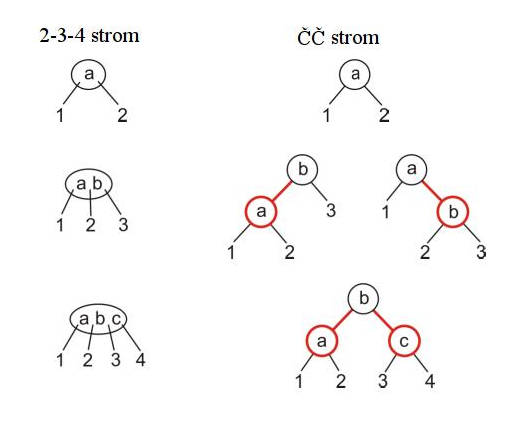
\includegraphics[scale=0.5]{img/RBstrom}
    \caption{Vytvoření RB stromu z B-stromu}
    \label{fig:rb_strom_z_b_stromu}
\end{figure}
\subsubsection{Vlastnosti RB stromu}
\begin{itemize}
	\item Kořenový uzel je vždy černý. Barva ostatních uzlů je dána barvou hrany, kterou je uzel spojen s předchůdcem.
	\item Mezi kořenem a libovolným listovým uzlem je stejný počet černých hran (a tím i černých uzlů).
	\item Ve stromu nikdy nenásledují dvě červené hrany po sobě (a tím i nikdy nenásledují dva červené uzly po sobě).
	\item Nechť mezi kořenem a listem je m černých hran. Pak mezi kořenem a libovolným listem je nejvýše m+1 červených hran.
\end{itemize}
\subsubsection{Přidání prvku}
Přidání probíhá standardním způsobem jako v běžném binárním vyhledávacím stromu. \\
Označení: x - přidávaný prvek \\
Vyhledáme prvek x ve stromu. Vyhledání může skončit třemi způsoby:
\begin{itemize}
	\item Prvek x byl ve stromu nalezen – nelze ho znovu přidat a přidávání tím končí.
	\item Vyhledávání skončilo v uzlu u, ve kterém je uložen prvek c, přičemž x < c a uzel u nemá levého následovníka. Vytvoříme nový uzel jako levého následovníka uzlu u a do něho dáme přidávaný prvek x.
	\item Vyhledávání skončilo v uzlu u s prvkem c, přičemž x > c a uzel u nemá pravého následovníka. Vytvoříme pravého následovníka uzlu u a do něho dáme přidávaný prvek x.
\end{itemize}
Přidávání je tedy realizováno vytvořením nového uzlu a jeho spojením hranou s uzlem u, ve kterém skončilo vyhledávání. Vytvořený uzel bude novým listem stromu. Aby zůstala zachována podmínka, že mezi kořenem a libovolným listem byl stejný počet černých hran, musíme nový uzel spojit s uzlem u červenou hranou a nový uzel bude červený uzel. Pokud uzel u je černý uzel, operace přidání je ukončena. Jestliže ale uzel u je červený uzel, jsou nyní ve stromu dvě červené hrany (dva červené uzly) po sobě.
\paragraph{Odstranění dvou červených uzlů po sobě}
rotace x výměna barev. \\
\begin{itemize}
	\item Horní z dvojice po sobě následujících červených uzlů nemá červeného sourozence – jednoduchá nebo dvojitá rotace.
	\item Horní z dvojice červených uzlů má červeného sourozence. Změníme jejich obarvení na černou barvu a barvu jejich předchůdce, pokud to není kořen, změníme na červenou barvu.
\end{itemize}
\subsubsection{Odebrání prvku}
Označení: x - odebíraný prvek
\begin{enumerate}
	\item Vyhledáme prvek x ve stromu. Vyhledání může skončit třemi způsoby:
	\begin{itemize}
		\item Prvek x nebyl ve stromu nalezen – není co odebrat.
		\item Prvek byl nalezen v uzlu v, který má nejvýše jednoho následníka. Tento uzel zrušíme.
		\item Prvek byl nalezen v uzlu v, který má dva následníky. V tomto případě do uzlu v přesuneme buďto nejpravější (největší) prvek z jeho levého podstromu anebo nejlevější (nejmenší) prvek z jeho pravého podstromu a uzel, z kterého byl prvek přesunut, zrušíme.
	\end{itemize}
	\item Další postup závisí na tom, jakou barvu má rušený uzel.
	\begin{itemize}
		\item Rušený uzel má červenou barvu. V tomto případě zrušení uzlu neovlivní počet černých uzlů (a černých hran) a odebrání je ukončeno.
		\item Rušený uzel má černou barvu a má červeného následníka. Následníka přebarvíme na černou barvu. Tím počet černých uzlů (a černých hran) zůstane zachován a odebrání je ukončeno.
		\item Rušený uzel v má černou barvu a nemá červeného následníka. Uzel v obarvíme jako dvojitý černý. Toto obarvení vyjadřuje, že zrušením uzlu by nastal deficit černé barvy na cestách od kořenu k listům, na kterých tento uzel leží. \\
		Další postup je transformacemi dosáhnout, aby ve stromu nebyl žádný uzel s dvojitým černým obarvením. Přitom u uzlu, který chceme zrušit, lze při odstranění jeho dvojitého černého obarvení ho ze stromu odstranit.
	\end{itemize}
\end{enumerate}
\paragraph{Odstranění dvojitého černého obarvení uzlu}
rotace x výměna barev.
\begin{itemize}
	\item Sourozenec uzlu s dvojitým černým obarvením je černý uzel a tento má přitom aspoň jednoho červeného následníka – jednoduchá nebo dvojitá rotace (spojená s určitým přebarvením uzlů).
	\item Sourozenec uzlu v s dvojitým černým obarvením je černý uzel a tento přitom nemá žádného červeného následníka. Jedno černé obarvení od obou uzlů (uzlu v a jeho sourozence) odebereme a k předchůdci těchto uzlů naopak jedno černé obarvení přidáme. Uzel v bude tímto mít jedno černé obarvení a jeho sourozenec bude červeně obarven.
	\begin{itemize}
		\item Předchůdce uzlu v je červený uzel – nyní bude černý uzel.
		\item Předchůdce uzlu v je černý uzel. Pokud to není kořen, bude mít nyní dvojité černé obarvení.
	\end{itemize}
	\item Sourozenec uzlu v s dvojitým černým obarvením je červený uzel – jednoduchá rotace.
\end{itemize}
\paragraph{Časová složitost operací} je závislá na výšce červeno-černého stromu. Odtud $\theta(ln(n))$.




\subsection{AVL stromy}
Jsou určitým způsobem vyvážené binární vyhledávací stromy.
Vyváženost v AVL stromu je zajištěna podmínkou, že pro každý uzel u stromu musí platit, že rozdíl mezi výškou jeho levého podstromu a výškou jeho pravého podstromu je nejvýše 1. Přitom výškou podstromu zde rozumíme maximum ze vzdáleností od uzlu u k uzlům daného podstromu, tedy vzdálenost mezi uzlem u a uzly, které jsou úplně naspodu podstromu. Pokud uzel nemá daného následníka (levého, pravého), je výška tohoto podstromu 0.
Při operaci přidání prvku do stromu je přidán nový uzel, při operaci odebrání prvku ze stromu je naopak uzel zrušen. Tyto operaci v příslušném místě, kde byl přidán nebo zrušen uzel, mění tvar stromu a mohou vést k porušení uvedené podmínky vyvážení u některého uzlu stromu. Proto je po operaci přidání nebo odebrání nutné ověřit, zda k této situaci nedošlo. Aby toto ověřování proběhlo efektivně, je v každém uzlu proměnná b (b=balance), která je označovaná jako faktor vyvážení uzlu a která obsahuje informaci o jeho stávajícím vyvážení.
Uzel je vyvážený, jestliže jeho faktor vyvážení je 1, 0 nebo -1. Při přidání prvku do stromu nebo odebrání prvku ze stromu se v důsledku změny tvaru stromu může v některém uzlu jeho faktor vyvážení změnit na 2 nebo -2. V tom případě je zapotřebí udělat transformaci, která obnoví vyvážení daného uzlu.
\subsubsection{Přidání prvku}
Operace přidání prvku do AVL stromu znamená na příslušném místě přidání uzlu do stromu, do kterého nový prvek vložíme, a následně aktualizujeme v příslušných částích stromu údaje o vyvážení v uzlech a ověřujeme, zda v některém uzlu nedošlo k narušení vyvážení stromu, a pokud ano, uzel vhodnou transformací vyvážíme. \\
Označení: x - přidávaný prvek
\begin{enumerate}
	\item Vyhledáme prvek x ve stromu. Vyhledání může skončit třemi způsoby:
	\begin{itemize}
		\item Prvek x byl ve stromu nalezen. Tím přidávání končí, neboť prvek x už je ve stromu obsažen a nelze ho přidat.
		\item Vyhledání skončilo v uzlu u, ve kterém je uložen prvek c, přičemž x < c a přitom uzel u už nemá levého následníka. V tom případě přidáme ke stromu nový uzel v jako levého následníka uzlu u a do něho nový prvek x vložíme.
		\item Vyhledání skončilo v uzlu u s prvkem c, přičemž x > c a přitom uzel u už nemá pravého následníka. V tom případě přidáme ke stromu nový uzel v jako pravého následníka uzlu u a do něho nový prvek x vložíme.
	\end{itemize}
	\item Po přidání uzlu procházíme uzly stromu na cestě od přidaného uzlu v směrem ke kořenu. Pro každý procházený uzel u na cestě aktualizujeme jeho faktor vyvážení.
	\begin{itemize}
		\item Pokud přidaný prvek je v levém podstromu aktuálního uzlu u, jeho faktor vyvážení zvýšíme o 1. \\
		Po aktualizaci faktoru vyvážení mohou nastat případy:
		\begin{itemize}
			\item Faktor vyvážení uzlu u je nyní 0. V tomto případě přidání prvku x nemá vliv na faktory vyvážení dalších uzlů na cestě ke kořenu a operace přidání tím skončila.
			\item Faktor vyvážení uzlu u je nyní 1. Je-li uzel u již kořen, operace přidání skončila. Jinak aktuální uzlem u učiníme předchůdce současného uzlu u a opět krok 2.
			\item Faktor vyvážení uzlu u je nyní 2. Uzel u je nevyvážený - vyvážíme ho vhodnou transformací (RR, RL). Po vyvážení:
			\begin{itemize}
				\item Je-li uzel u již kořen, operace přidání skončila.
				\item Je-li po vyvážení hodnota faktoru vyvážení uzlu u rovna 0, operace přidání je ukončena (maximum z výšek podstromů uzlu u se transformací snížilo o 1, tudíž už to nemá vliv na faktor vyvážení předchůdce uzlu u). Jinak přejdeme k předchůdci uzlu u a opět krok 2.
			\end{itemize}
		\end{itemize}
		\item Pokud přidaný prvek je v pravém podstromu aktuálního uzlu u, jeho faktor vyvážení snížíme o 1. \\
		Po aktualizaci faktoru vyvážení mohou nastat případy:
		\begin{itemize}
			\item Faktor vyvážení uzlu u je nyní 0. V tomto případě přidání prvku x nemá vliv na faktory vyvážení dalších uzlů na cestě ke kořenu a operace přidání tím skončila.
			\item Faktor vyvážení uzlu u je nyní -1. Je-li uzel u již kořen, operace přidání skončila. Jinak aktuální uzlem u učiníme předchůdce současného uzlu u a opět krok 2.
			\item Faktor vyvážení uzlu u je nyní -2. Uzel u je nevyvážený - vyvážíme ho vhodnou transformací (LL, LR). Po vyvážení:
			\begin{itemize}
				\item Je-li uzel u již kořen, operace přidání skončila.
				\item Je-li po vyvážení hodnota faktoru vyvážení uzlu u rovna 0, operace přidání je ukončena (maximum z výšek podstromů uzlu u se transformací snížilo o 1, tudíž už to nemá vliv na faktor vyvážení předchůdce uzlu u). Jinak přejdeme k předchůdci uzlu u a opět krok 2.
			\end{itemize}
		\end{itemize}
	\end{itemize}
\end{enumerate}
\subsubsection{Odebrání prvku}
Operace odebrání prvku z AVL stromu znamená na příslušném místě zrušení uzlu ve stromu. Následně aktualizujeme v příslušných částích stromu údaje o vyvážení v uzlech a ověřujeme, zda v některém uzlu nedošlo k narušení vyvážení stromu, a pokud ano, uzel vhodnou transformací vyvážíme. \\
Označení: x - odebíraný prvek
\begin{enumerate}
	\item Vyhledáme prvek x ve stromu. Vyhledání může skončit třemi způsoby:
	\begin{itemize}
		\item Prvek x nebyl ve stromu nalezen – není co odebrat.
		\item Prvek byl nalezen v uzlu v, který má nejvýše jednoho následníka.Tento uzel zrušíme.
		\item Prvek byl nalezen v uzlu v, který má dva následníky. V tomto případě do uzlu v přesuneme buďto nejpravější (největší) prvek z jeho levého podstromu anebo nejlevější (nejmenší) prvek z jeho pravého podstromu a uzel, z kterého byl prvek přesunut, zrušíme.
	\end{itemize}
	\item Po zrušení uzlu procházíme uzly stromu na cestě od zrušeného uzlu směrem ke kořenu. Pro každý procházený uzel u na cestě aktualizujeme jeho hodnotu vyvážení b.
	\begin{itemize}
		\item Pokud zrušený uzel byl v levém podstromu aktuálního uzlu u, jeho faktor vyvážení snížíme o 1. \\
		Po aktualizaci faktoru vyvážení mohou nastat případy:
		\begin{itemize}
			\item Faktor vyvážení uzlu u je nyní -1. V tomto případě zrušení uzlu nemá vliv na faktory vyvážení dalších uzlů na cestě ke kořenu a operace odebrání tím skončila.
			\item Faktor vyvážení uzlu u je nyní 0. Je-li uzel u již kořen, operace odebrání skončila. Jinak aktuální uzlem u učiníme předchůdce současného uzlu u a opět krok 2.
			\item Faktor vyvážení uzlu u je nyní -2. Uzel u je nevyvážený - vyvážíme ho vhodnou transformací (LL, LR). Po vyvážení:
			\begin{itemize}
				\item Je-li uzel u již kořen, operace odebrání skončila.
				\item Je-li po vyvážení faktor vyvážení uzlu u roven -1, operace přidání je ukončena (maximum z výšek podstromů uzlu u se transformací zvýšilo o 1, tudíž už to nemá vliv na faktor vyvážení předchůdce uzlu u). Jinak přejdeme k předchůdci uzlu u a opět krok 2.
			\end{itemize}
		\end{itemize}
		\item Pokud zrušený uzel je v pravém podstromu aktuálního uzlu u, jeho faktor vyvážení zvýšíme o 1. \\
		Po aktualizaci faktoru vyvážení mohou nastat případy:
		\begin{itemize}
			\item Faktor vyvážení uzlu u je nyní 1. V tomto případě zrušení uzlu nemá vliv na faktory vyvážení dalších uzlů na cestě ke kořenu a operace přidání tím skončila.
			\item Faktor vyvážení uzlu u je nyní 0. Je-li uzel u již kořen, operace odebrání skončila. Jinak aktuální uzlem u učiníme předchůdce současného uzlu u a opět krok 2.
			\item Faktor vyvážení uzlu u je nyní 2. Uzel u je nevyvážený - vyvážíme ho vhodnou transformací (RR, RL). Po vyvážení:
			\begin{itemize}
				\item Je-li uzel u již kořen, operace přidání skončila.
				\item Je-li po vyvážení faktor vyvážení uzlu u roven 1, operace přidání je ukončena (maximum z výšek podstromů uzlu u setransformací zvýšilo o 1, tudíž už to nemá vliv na faktor vyvážení předchůdce uzlu u). Jinak přejdeme k předchůdci uzlu u a opět krok 2.
			\end{itemize}
		\end{itemize}
	\end{itemize}
\end{enumerate}
\paragraph{Časová složitost operací} $\theta(log(n))$.




\subsection{B-stromy}
B-stromy jsou velmi významným typem vyhledávacích stromů. Mají v uzlech uloženo více prvků. Struktura B-stromů je definována následujícími vlastnostmi:
\begin{itemize}
	\item Kapacita uzlu (počet prvků, který lze do uzlu uložit) je u všech uzlů stromu stejná a volíme ji před začátkem vytváření stromu, kapacitu označme r $(r \geq 2)$ Protože v B-stromech má významnou úlohu polovina z tohoto počtu, zaveďme si pro ni samostatné označení $p = \frac{r}{2}$ pro r sudé a $p = \frac{r-1}{2}$ pro r liché.
	\item Důležité pro efektivní využití uzlů je jejich zaplnění. Všechny uzly vyjma kořene musí být aspoň z poloviny zaplněny prvky pro r sudé nebo p prvky pro r liché, tedy počet prvků v uzlech uložených musí být v rozmezí p až r prvků. Jedině u kořene stačí, aby obsahoval aspoň jeden prvek, tedy jeho zaplnění je v rozmezí 1 až r prvků.
	\item Prvky uložené v uzlu jsou v něm seřazeny vzestupně dle velikosti.
	\item Uzel je buďto list anebo má o jednoho následníka více, než je počet prvků v něm uložený. \\
	Přitom pro prvky v jednotlivých podstromech, které těmito následníky začínají, platí:
	\begin{itemize}
		\item Pro každý prvek d v podstromu začínajícího uzlem $násl_0$ platí $d < c_1$.
		\item Pro každý prvek d v podstromu začínajícího uzlem $násl_1$ platí $c_1 < d < c_2$.
		\item ............
		\item Pro každý prvek d v podstromu začínajícího uzlem $násl_{k-1}$ platí $c_{k-1} < d <c_k$.
		\item Pro každý prvek d v podstromu začínajícího uzlem $násl_k$ platí $d > c_k$.
	\end{itemize}
	\item Listy jsou v B-stromu jen v jeho poslední (nejspodnější) úrovni.
\end{itemize}
Podle maximálního počtu následníků označujeme i řád B-stromu. B-strom s kapacitou uzlu r má řád r + 1, neboť nelistový uzel může mít až r + 1 následníků.
\subsubsection{Vyhledání prvku}
\begin{enumerate}
	\item Počáteční krok \\
	Uzel, který je v daném okamžiku vyhledávání aktuální, budeme označovat u. Na začátku jím bude kořen stromu. \\
	Hledaná hodnota nechť je x.
	\item Průběžný krok \\
	Provedeme vyhledání hodnoty mezi prvky uloženými v aktuálním uzlu u. Protože prvky jsou v uzlu setříděné, lze k tomu použít binární vyhledávání. To použijeme v případě, kdy kapacita uzlů je zvolena dostatečně velká, aby se to vyplatilo. Vyhledání může skončit třemi způsoby:
	\begin{itemize}
		\item Prvek byl v aktuálním uzlu u nalezen, čímž vyhledávání úspěšně končí.
		\item Prvek nebyl v aktuálním uzlu u nalezen a tento uzel je list. Tím vyhledávání končí - hledaný prvek není ve stromu obsažen.
		\item Prvek nebyl v aktuálním uzlu u nalezen a tento uzel je nelistový. V tom případě vyhledávání skončilo v místě, kde je odkaz na následníka, ve kterém vyhledávání má pokračovat (tj. na následníka, kterým začíná podstrom, jež by hledaný prvek měl obsahovat). Tohoto následníka učiníme novým aktuální uzlem a opět se provede krok 2.
	\end{itemize}
\end{enumerate}
\subsubsection{Přidání prvku}
Chceme-li do B-stromu přidat prvek, znamená to najít příslušný uzel, do kterého nový prvek patří, a následně ověřit, zda přitom nedošlo k přeplnění, a pokud ano, provést rozdělení uzlu.
\begin{enumerate}
	\item Přidání prvku \\
	Označme přidávaný prvek x. Provedeme je vyhledání ve stromu. Použijeme k tomu běžný algoritmus pro vyhledání. Ten může skončit dvěma způsoby:
	\begin{itemize}
		\item Prvek x byl ve stromu nalezen. Tím přidávání končí, neboť prvek x už je ve stromu obsažen (u vyhledávacích stromů se nepředpokládá vícenásobný výskyt stejného prvku).
		\item Vyhledávání skončilo v listovém uzlu u v místě, kam nový prvek podle velikosti vzhledem k ostatním prvků patří. Prvek na toto místo vložíme. Pokud uzel u předtím nebyl zcela zaplněn, operace přidání tím končí. Jinak provedeme rozdělení uzlu.
	\end{itemize}
	\item Rozdělení uzlu \\
	Jestliže uzel u má po přidání r+1 prvků, tedy došlo k jeho přeplnění uzlu, rozdělíme ho na tři části: \\
	p prvků na začátku uzlu + prvek uprostřed uzlu + p prvků na konci uzlu. \\
	Části s p prvky budou tvořit nové listy. Prvek, jež je v uzlu u uprostřed, se přesune do předchůdce na místo, kde byl původní odkaz na list. Po přesunu nalevo a napravo od něho vytvoříme nové odkazy na nově vzniklé listy.
\end{enumerate}
Zřejmě po přidání uzlu do předchůdce v něm může dojít rovněž k jeho přeplnění, pokud předtím byl zcela zaplněn. To se řeší stejným způsobem - rozdělením tohoto uzlu na tři části s počtem prvků p+1+p. Dvě jeho části s p prvky budou tvořit nové uzly a zbývající prostřední prvek vložíme do jeho předchůdce. Takto postupujeme směrem nahoru, až buďto narazíme na uzel, u kterého po vložení dalšího prvku nedojde k přeplnění, anebo se nakonec dostaneme až ke kořenu. Pokud i u něho dojde k přeplnění, rozdělí se a střední prvek v tomto rozdělení bude nyní nový kořen. V této situaci dojde ke zvětšení výšky stromu.
\subsubsection{Odebrání prvku}
Chceme-li z B-stromu odebrat prvek, znamená to vyhledat uzel, ve kterém se prvek nachází, prvek z něho odstranit a následně ověřit, zda odebráním prvku nepoklesl počet prvků v daném uzlu pod přípustnou mez, a pokud ano, je nutné to vyřešit.
\begin{enumerate}
	\item Odebrání prvku: \\
	Označme odstraňovaný prvek x. Provedeme jeho vyhledání ve stromu. Použijeme k tomu běžný algoritmus pro vyhledání. Ten může skončit třemi způsoby:
	\begin{itemize}
		\item Prvek x nebyl ve stromu nalezen - není co odebrat.
		\item Prvek x byl nalezen v listovém uzlu. Prvek z uzlu odstraníme. Pokud list je po zrušení prvku aspoň z poloviny zaplněn, operace odebrání končí. Jinak přejdeme ke kroku 2.
		\item Prvek x byl nalezen v uzlu u, který není listem. Prvek x z uzlu odstraníme a na volné místo v uzlu u přesuneme buďto největší prvek z jeho levého podstromu, což je poslední prvek v nejpravějším listu podstromu, anebo nejmenší prvek z jeho pravého podstromu, což je první prvek v nejlevějším listu podstromu. Pokud list, odkud jsme prvek přesunuli, je stále aspoň z poloviny zaplněn, operace odebrání prvku končí. Jinak přejdeme ke kroku 2.
	\end{itemize}
	\item Zmenšení počtu prvků v uzlu \\
	Sem se dostáváme v situaci, kdy po odstranění prvku ze stromu je nyní ve stromu list v, který má jen p-1 prvků. Jak se tento stav řeší, závisí na zaplnění přímých sousedů listu. Jsou dvě možnosti:
	\begin{itemize}
		\item List v má aspoň jednoho přímého souseda, který má více než p prvků. Přímým sousedem zde máme na mysli uzel, který je nejen vedle uzlu v, ale má i stejného předchůdce. Pak do listu v přesuneme prvek z předchůdce a na prázdné místo v předchůdci přesuneme příslušný prvek ze souseda. Následující obrázek ukazuje tento přesun pro oba možné přímé sousedy, nejdříve pro levého souseda, pak pro pravého souseda.
		\item List v má jen přímé sousedy, které mají právě p prvků. Pak vytvoříme nový list s r prvky tak, že sloučíme prvky z listu v + prvek z předchůdce + prvky ze souseda. \\
		Je zřejmé, že tímto ubyl jeden prvek v předchůdci. Pokud tento má nyní jen p-1 prvků, řeší se to analogicky v závislosti na tom, kolik prvků mají jeho přímí sousedé. Takto se můžeme případně dostat až k uzlu, který je následníkemkořene. Pokud je vytvořen nový uzel sloučením s jeho přímým sousedem a pokud kořen v této chvíli má jen jeden prvek, dojde přitom k vytvoření nového kořene a zároveň ke snížení výšky stromu. Na následujícím obrázku je tato situace pro případ, kdy je pro sloučení vzat levý přímý soused.
	\end{itemize}
\end{enumerate}
\paragraph{Časová složitost operací} $\theta(log(n))$.




\subsection{Hašování}
Datová struktura použitá v hašování pro uložení prvků je tabulka. Tabulka se skládá z řádků. U hašování pro řádky tabulky používáme označení přihrádky. V každé přihrádce je místo pro uložení jednoho datového prvku. Počet přihrádek v tabulce, tedy kapacitu tabulky označme m. Na jednotlivé přihrádky v tabulce se odkazujeme (adresujeme je) čísly 0 až m-1. Při implementaci hašování se tabulka snadno realizuje pomocí pole. Datový typ prvků pole se zvolí takový, aby se do něho daly uložit údaje, které ukládáme do přihrádek tabulky. Tím každý prvek pole reprezentuje jednu přihrádku tabulky a indexování prvků pole odpovídá adresování jednotlivých přihrádek v tabulce. \\
Základem hašování je hašovací funkce. Je to zobrazení, které hodnotě prvku (nebo vyhledávacímu klíči prvku, pokud prvek je strukturovaný typ) přiřadí číslo některé z přihrádek v tabulce, tedy číslo v rozmezí 0 až m-1. Hašovací funkce se typicky sestaví ze dvou funkcí. Ta první hodnotu prvku zobrazí na celé (nezáporné) číslo. Druhá celé číslo zobrazí na číslo přihrádky v tabulce, tedy na celé číslo z intervalu <0,m-1>. \\
Cílem hašovací funkce je rovnoměrné rozmístění prvků v tabulce. Z toho plyne, že první funkce, která převádí hodnotu prvku na celé číslo, by měla mít vlastnosti:
\begin{itemize}
	\item Zobrazovat hodnoty prvků na co největší počet různých celých čísel.
	\item Zobrazení na celá čísla by mělo být rovnoměrné (na jednotlivá čísla by se měl zobrazovat přibližně stejný počet prvků, které chceme do hašovací tabulky uložit).
\end{itemize}
Dalším přirozeným požadavkem na hašovací funkci je, aby její výpočet nebyl příliš časově náročný.
\subsubsection{Hašovací funkce pro řetězce}
Řetězec si označme $z_1 z_2 \cdots z_k$, kde $z_i$ je znak z řetězce a k je délka řetězce.
\paragraph{První část hašovací funkce}
Jedna z jednodušších funkcí zobrazující řetězec na celé číslo je $c_1 ( z_1 z_2 \cdots z_k ) = p \ast asc ( z_1 ) + q \ast asc ( z_2 ) + asc ( z_k ) + k$, kde p a q jsou zvolené konstanty, nejlépe prvočísla (např. p=127, q=31), protože ty mají nejlepší předpoklady pro rovnoměrné zobrazení do množiny celých čísel. Funkce asc převádí znak na jeho ASCII hodnotu (nebo Unicode hodnotu). \\
Dokonalejší, ale na druhé straně náročnější na výpočet, je funkce $c_2 ( z_1 z_2 \cdots z_k ) = p^{k-1} \ast asc ( z_1 ) + p^{k-2} \ast asc ( z_2 ) + \cdots + p \ast asc ( z_{k-1} ) + asc ( z_k )$, kde p je konstanta, opět nejlépe prvočíslo (např. p=31).
\paragraph{Drugá část hashovací funkce}
která převádí celé číslo na číslo přihrádky v hašovací tabulce, je velmi jednoduchá. Používá se pro ni operace modulo. Obecný zápis hašovací funkce je $h ( x ) = c ( x ) mod m$, kde c(x) je první část hašovací funkce a m je rozsah (počet přihrádek) hašovací tabulky. Opět je nejlepší zvolit m prvočíslo, protože to nemá žádného netriviálního vlastního dělitele, čímž poskytuje nejlepší předpoklady pro rovnoměrné rozmístění prvků v tabulce. \\ \\
Vedle prvočíselného počtu přihrádek v tabulce se v praxi používá i počet přihrádek, který je mocninou čísla 2. Tento počet nemá tak dobré předpoklady pro rovnoměrné rozmístění prvků v tabulce, ale výpočet hašovací funkce je snadnější, protože místo operace modulo lze použít jednodušší operaci bitového součinu.
\subsubsection{Metoda otevřeného adresování}
V případě, kdy pozice v tabulce vypočítaná hašovací funkcí je obsazena, počítá další pozice tak dlouho, dokud se nenajde volná pozice anebo se nezjistí, že tabulka už je zaplněna.
\paragraph{Lineární hledání}
nové pozice počítáme funkcí $H(x, i) = (h(x) + i)\:mod\:m$, kde h(x) je výchozí hašovací funkce, i je celočíselný parametr a m je rozsah tabulky. \\
Lineární umísťování za sebou vede k vytváření nežádoucích shluků. \textbf{Shlukem} nazýváme větší počty za sebou následujících obsazených přihrádek tabulky. Pokud je vypočítaná primární pozice obsazená a je přitom uvnitř takového shluku, znamená to při lineárním hledání, že musíme projít všechny přihrádky v tomto shluku za primární pozicí, než se dostaneme k nějaké volné sekundární pozici, abychom prvek do ní mohli uložit. Přitom shluky prodlužují nejen operaci přidání prvku do tabulky, ale také vyhledávání prvku v tabulce. Při vyhledávání začínáme na primární pozici a pokud na ní prvek není a tato pozice je přitom obsazena (je na ní jiný prvek), procházíme sekundární pozice tak dlouho, dokud prvek nenajdeme nebo se nedostaneme k volné pozici, což je příznakem toho, že hledaný prvek v tabulce není.
\paragraph{Kvadratické hledání}
Proto místo lineárního hledání se často používá kvadratické hledání. U něho sice také vznikají shluky, ale už v menší míře. Hašovací funkce používaná pro kvadratické hledání má většinou jednoduchý tvar $H(x, i) = (h(x) + i^2 )\:mod\:m$. U ní je už určitý problém, že během hledání se můžeme touto funkcí dostat znovu na stejnou pozici, kterou jsme již prošli, aniž jsme přitom vyčerpali celou tabulku.
\paragraph{Dvojí hašování}
je propracovanější metoda. Hašovací funkce má tvar $H(x, i) = (h(x) + i \ast h_2(x))\:mod\:m$, kde $h_2$ je sekundární hašovací funkce v rozmezí hodnot 1 až m-1. V praxi nejčastějí vychází z primární funkce. Máme funkci $c(x)$, primírní hašovací funkci $h(x) = c(x)\:mod\:m$. Sekundární hašovací funkce vznikne jako $h_2(x) = 1 + (c(x)\:mod\:(m -1))$. Pozici nyní můžeme počítat rekurzivně \\
$H(x,0) = h(x)$ \\ $H(x, i) = (H(x, i-1) + h_2(x))\:mod\:m\;$	pro i = 1,2,3,...
\paragraph{Vyhledávání v tabulce}
Při vyhledávání v hašovací tabulce nejprve vypočítáme hodnotu hašovací funkce pro hledaný prvek x. Podíváme se do tabulky na přihrádku, na kterou ukazuje hodnota hašovací funkce. Mohou nastat případy:
\begin{itemize}
	\item Přihrádka je prázdná – hledaný prvek není v tabulce.
	\item V přihrádce je hledaný prvek x – vyhledávání tím úspěšně končí.
	\item V přihrádce je jiný prvek než x. Začneme postupně počítat další možné pozice a srovnávat prvky na nich s hledaným prvkem x, dokud buďto hledaný prvek nenalezneme anebo se nedostaneme na prázdnou přihrádku anebo nevyčerpáme všechny možné pozice.
\end{itemize}
\subsubsection{Zřetězení}
Předchozí metoda otevřeného adresování má dvě nevýhody:
\begin{itemize}
	\item Počet prvků, jež lze do tabulky uložit, je omezen její velikostí. Pokud dopředu neznáme, kolik prvků bude do tabulky ukládáno, může se stát, že ji stanovíme malou a dojde k jejímu přeplnění. Následné zvětšení velikosti tabulky je většinou časově náročně.
	\item Při vyhledávání, zejména v dost zaplněné tabulce, procházíme v důsledku otevřeného adresování i prvky, které mají jinou hodnotu hašovací funkce, čímž se doba vyhledávání zvětšuje.
\end{itemize}
Tyto nevýhody odstraňuje metoda zřetězení, která k ukládání dalších prvků se stejnou hodnotou hašovací funkce využívá seznamy. Hašovací tabulka v tomto případě obsahuje ukazatele na začátek (první uzel) jednotlivých seznamů. \\
Pokud potřebujeme do hašovací tabulky prvky nejen přidávat, ale i odebírat je, pak je nejvhodnější použít metodu zřetězení pro řešení kolicí. Odebrání se pak realizuje vyhledáním prvku v příslušném seznamu a zrušením uzlu, který odebíraný prvek obsahuje.\\
V případě, že odebírání bude v hašovací tabulce s otevřeným adresováním, je realizace odebírání o něco komplikovanější. Budeme rozeznávat tři různé stavy přihrádky tabulky:
\begin{itemize}
	\item Přihrádka je prázdná – v této přihrádce nikdy nebyl uložen žádný prvek.
	\item Přihrádka je volná – v této přihrádce byl uložen prvek, ale ten byl pak z tabulky odebrán.
	\item Přihrádka je obsazena – v této přihrádce je uložen prvek.
\end{itemize}
Při vyhledávání budeme volné přihrádky přeskakovat. Vyhledávání skončí, až když hledaný prvek najdeme nebo se dostaneme na prázdnou přihrádku (nebo jsme prošli celou tabulku, či její podstatnou část). Při přidávání budeme hledat první prázdnou nebo volnou přihrádku.
\paragraph{Časová složitost} vyhledávání je dána složitostí hašovací funkce (můžeme považovat za konstantní - řetězce mají omezenou délku). Při vkládání bez kolizí $\theta (1)$. Složitost roste s počtem kolizí v tabulce. Volba hašovací tabulky je zejména podstatná u metody otevřeného adresování. Volíme ji aspoň o 10\% větší, než je očekávaný počet prvků.
\paragraph{Perfektní hašování} Je hašování bez kolizí. Používá se v případech, kdy jsou známy prvky, které budou uloženy do hašovací tabulky. Pro tyto prvky se navrhne samostatná hašovací funkce, při jejímž použití nenastanou žádné kolize.
\paragraph{Minimální perfektní hašování} Je perfektní hašování, kdy navíc po uložení prvků nezůstanou v tabulce žádné volné přihrádky. Počet přihrádek v tabulce je tedy roven počtu uložených prvků. Nalezení takové hašovací funkce je ale obtížné.
\subsubsection{Extendible hashing}
Metoda hašování nazývaná extendible hashing nevyžaduje počáteční stanovení velikosti hašovací tabulky a navíc poskytuje konstantní časovou složitost vyhledání prvku bez ohledu na to, kolik prvků je do tabulky vloženo. Hašovací datová struktura se skládá ze dvou částí - adresáře a přihrádky. Adresář je pole odkazů na přihrádky. Velikost pole adresáře je $2^d$ odkazů. Hodnota d se dynamicky mění v závislosti na počtu prvků uložených v hašovací struktuře. Na začátku je zpravidla d malé. Při postupném zvyšování počtu ukládaných prvků do hašovací struktury se v určitých okamžicích hodnota d zvyšuje. Přihrádka je místo pro uložení pevně stanoveného počtu datových prvků. Velikost všech přihrádek je stejná. Základem metody je opět hašovací funkce, která datový prvek zobrazí na celé číslo. Posledních d bitů tohoto čísla je indexem v poli adresáře, kde najdeme odkaz na přihrádku, ve které je uložen daný prvek.
\paragraph{Vyhledání prvku v hašovací struktuře}
Jednotlivé bity hodnoty hašovací funkce si označíme: \\
$\cdots b_{d+1} b_d b_{d-1} \cdots b_3 b_2 b_1$ ($b_1$ je nejméně významný bit)
\begin{itemize}
	\item Vypočítáme hodnotu hašovací funkce hledaného prvku.
	\item Vezmeme posledních d bitů $b_d\cdots b_1$ vypočtené hodnoty hašovací funkce. Ty jsou indexem v poli adresáře. V něm v prvku, který odpovídá tomuto indexu, zjistíme odkaz na příslušnou přihrádku.
	\item V přihrádce procházíme v ní uložené prvky a srovnáváme je s hledaným prvkem, dokud nenalezneme prvek shodný s hledaným prvkem nebo je všechny neprojdeme (pak hledaný prvek není nalezen).
\end{itemize}
\paragraph{Přidání prvku do hašovací struktury}
\begin{itemize}
	\item Vypočítáme hodnotu hašovací funkce přidávaného prvku.
	\item Vezmeme posledních d bitů $b_d \cdots b_1$ vypočtené hodnoty hašovací funkce. Ty jsou indexem v poli adresáře. V něm v prvku pole, který odpovídá tomuto indexu, zjistíme odkaz na příslušnou přihrádku.
	\item Je-li v přihrádce místo pro uložení přidávaného prvku, prvek do přihrádky vložíme. Jinak je nutné přihrádku rozdělit.
\end{itemize}
\paragraph{Rozdělení přihrádky}
\begin{itemize}
	\item Pokud mají všechny prvky uložené v přihrádce stejnou hodnotu posledních d bitů $b_d \cdots b_1$ hodnot svých hašovacích funkcí, přihrádku rozdělíme na dvě a do první dáme prvky, jejichž hašovací funkce má hodnotu dalšího bitu $b_{d+1}$ rovnu 0. Do druhé dáme prvky, jejichž hodnota bitu $b_{d+1}$ je 1. Po rozdělení přihrádek následně i zdvojnásobíme velikost adresář (hodnotu d zvýšíme o 1). Při zdvojnásobení velikosti adresáře zachováme odkazy na přihrádky, které se nerozdělily. Pokud by bit $b_{d+1}$ byl u všech prvků stejný, vzali bychom další bit $b_{d+2}$ a adresář bychom zvětšili čtyřikrát (hodnotu d bychom zvýšili celkově o 2). Atd.
	\item Jestliže prvky uložené v přihrádce nemají shodnou hodnotu posledních d bitů hodnot svých hašovacích funkcí, rozdělíme je do dvou přihrádek podle prvního (bráno zleva) z d bitů, který není u všech prvků identický. Nechť je to bit b i, kde $i \leq d$ a i je největší index takový, že hodnota tohoto bitu hašovacích funkcí všech prvků není stejná. Následně v adresáři příslušně upravíme odkazy na tyto přihrádky.
\end{itemize}
\paragraph{Odebrání prvku z hašovací struktury}
\begin{itemize}
	\item Vyhledáme odebíraný prvek.
	\item Pokud byl nalezen, odstraníme ho z dané přihrádky.
\end{itemize}
Při větším odebírání, kdy vznikne více prázdných přihrádek, lze některé přihrádky sloučit. Případně po větším sloučení je někdy možné zmenšit velikost adresáře na polovinu. Jednoduchým způsobem lze sloučit prázdnou přihrádku, na kterou je jen jeden odkaz z adresáře, s přihrádkou, na kterou je opět jen jeden odkaz z adresáře a zároveň hodnoty indexů těchto odkazů v adresáři se liší jen v jednom bitu. Bylo by možné sloučit i v případě, že na obě slučované přihrádky je stejný počet $2^m$ odkazů a přitom hodnoty indexů jednotlivých odkazů v adresáři se liší právě v m bitech. Běžně se ale slučování přihrádek při odebírání nedělá.
\paragraph{Uložení na vnější paměti}
Použití této metody je vhodné, pokud by standardní hašovací tabulka byla tak rozsáhlá, že by se nevešla do paměti. U rozšiřitelného hašování stačí, aby v paměti byl uložen jen adresář. Přihrádky mohou být uloženy v souboru na vnější paměti.\\





\newpage
%----------------------------------------treti odstavec---------------------------------------------------
\section{}
\paragraph{Programovací jazyky, jejich syntaxe a sémantika. Přehled paradigmat: funkcionální, procedurální, logické, objektové. Symbolické výrazy a vyhodnocovací proces jazyka Scheme. Vytváření abstrakcí pomocí procedur. Procedury vyšších řádů: aplikace a mapování. Seznamy a hierarchická data. Indukce a rekurze: princip a příklady. Typy rekurzivních výpočetních procesů. Lexikální a dynamický rozsah platnosti. Vlastnosti typových systémů.}
  \subsection{Programovací jazyky, jejich syntaxe a sémantika}
    \paragraph{Programovací jazyk}
    Programovací jazyk jsou smluvená pravidla, v souladu se kterými je vytvořen program. Program je předpisem s přesně daným tvarem a významem, podle kterého vzniká výpočetní proces. Výpočetní proces je proces, při kterém jsou zpracováváná vstupní data. Každý programovací jazyk musí mít popsánu svoji syntax a sémantiku.\\
    Dělení:
    \begin{itemize}
      \item dle míry abstrakce
      \begin{itemize}
        \item nižší -- kód stroje, jazyk symbolických adres, autokód, bajtkód
        \begin{itemize}
          \item těsně vázané na hardware počítače
          \item programové konstrukce jsou spjaty s instrukční sadou procesoru
          \item prakticky žádné prostředky abstrakce $\rightarrow$ zdlouhavé programování $\rightarrow$ zanášení chyb do programu (špatně odhalitelné)
          \item vazba na hardware umožňuje počítač \uv{plně využít}
        \end{itemize}
        \item vyšší -- většina jazyků
        \begin{itemize}
          \item nejsou vázané na hardware
          \item výrazně vyšší stupeň abstrakce $\rightarrow$ snadnější a rychlejší tvorba programů $\rightarrow$ menší riziko vzniku chyb
          \end{itemize}
          \item každý vyšší jazyk by měl programátorovi dát k dispozici:
          \begin{itemize}
            \item \textit{primitivní výrazy} (např. čísla, symboly, \ldots)
            \item \textit{prostředky pro kombinaci} primitivních výrazů do složitějších
            \item \textit{prostředky pro abstrakci} (možnost pojmenování složených výrazů a možnost s nimi dále manipulovat)
          \end{itemize}
        \end{itemize}
        \item dle způsobu překladu a spuštění
        \begin{itemize}
          \item překlad přes nižší programovací jazyk (např. Pascal, C, Java, Cobol)
          \begin{itemize}
            \item \textit{překladač} (\textit{kompilátor, compiler}) \textit{programovacího jazyka} je program, který načte celý program a poté provede jeho překlad do některého nižšího programovacího jazyka, typicky do \textit{assembleru} nebo do nějakého bajtkódu, při překladu mohou nastat tři situace
            \begin{itemize}
              \item překlad byl proveden do \textit{kódu stroje}, pak překlad končí, protože jeho výsledkem je již program zpracovatelný procesorem, může být přímo spuštěn
              \item překlad byl proveden do \textit{assembleru}, pak je potřeba dodatečný překlad do kódu stroje, který obvykle provádí rovněž překladač
              \item překlad byl proveden do \textit{bajtkódu}, pak překlad končí, bajtkód ale není přímo zpracovatelný procesorem, musí tedy být ještě \textit{interpretován} nebo \textit{přeložen} (méně časté) dalším programem.
            \end{itemize}
            \item konstrukčně složitější než interpret
            \item výsledkem je větší rychlost, ale také náročnost na správně zapsaný kód
          \end{itemize}
          \item překlad přes vyšší programovací jazyk
          \begin{itemize}
            \item typickou volbou překlad do některého z cílových jazyků, jejichž překladače jsou široce rozšířené, např. C
          \end{itemize}
          \item interpretace (např. BASIC, Perl, Python, shell, Ruby)
          \begin{itemize}
            \item \textit{interpret programovacího jazyka} je program, který čte výrazy programu a postupně je přímo vykonává, interprety tedy (obvykle) z daného programu neprodukují kód v jazyku stroje
            \item kvůli efektivitě výsledného výpočetního procesu se může dodatečně kompilovat během interpretace, takovou kompilaci označujeme anglickým termínem \textit{just in time compilation}.
          \end{itemize}
        \end{itemize}
      \end{itemize}
    \paragraph{Syntaxe}
    Soubor přesně daných pravidel definujících, jak zapisujeme programy v daném programovacím jazyku. Syntax většiny programovacích jazyků je popsána v jejich standardech pomocí \textit{formálních gramatik}, případně jejich vhodným rozšířením, například \textit{Backus-Naurovy formy}.
    \begin{itemize}
      \item \textit{syntaktická chyba} je chybou v zápisu programu -- kód, který není z pohledu daného jazyka syntakticky správný, nelze v podstatě chápat ani jako program v daném jazyku -- odhalí překladač během překladu, interpret odhalí až v momentě, kdy se pokusí načíst chybný vstupní výraz
    \end{itemize}
    \paragraph{Sémantika}
      \textit{Význam programu}. V případě ohodnocování syntakticky neplatných řetězců není výpočet proveden. Sémantika popisuje procesy, které řídí počítač při vykonávání programu v daném programovacím jazyce. Například tím, že popisuje vztah mezi vstupem a výstupem programu, nebo popisem jak program poběží na určité platformě, tedy vytvořením modelu výpočtu.
  \subsection{Přehled paradigmat: funkcionální, procedurální, logické, objektové}
  \subsection{Symbolické výrazy a vyhodnocovací proces jazyka Scheme}
  \subsection{Vytváření abstrakcí pomocí procedur}
  \subsection{Procedury vyšších řádů: aplikace a mapování}
  \subsection{Seznamy a hierarchická data}
  \subsection{Indukce a rekurze: princip a příklady}
  \subsection{Typy rekurzivních výpočetních procesů}
  \subsection{Lexikální a dynamický rozsah platnosti}
  \subsection{Vlastnosti typových systémů}


%---------------------------------------------------------------------------------------------
%---------------------------------------- Čtvrtý odstavec-------------------------------------
%---------------------------------------------------------------------------------------------
\newpage
\section{Makra}
\paragraph{Motivace} Chceme upravit $if$ tak aby při absenci alternativního výrazu vracel $\#f$.
\\ Nyní máme (\color{red}$if$ \color{black} (= 1 2) '$blah$) $\Rightarrow$ nedefinovaná hodnota.
\\ Chceme: (\color{red}$new-if$ \color{black} (= 1 2) '$blah$) $\Rightarrow$ $\#f$.
\\ Potřebujeme zavést předpis, který bude provádět "transformaci kódu". Spoustu možností jak vyřešit (nová transformační procedura nebo třeba pomocí kvazikvótování). Nejlepší řešení $\rightarrow$ zavedeni \color{blue} maker \color{black}.
\subsection{Dva základní pohledy na makra}
\subsubsection{První pohled}
\begin{center}
	Makra jsou "rozšířením syntaxe jazyka"
\end{center}
\begin{definition}
	makro = dáno definicí svého transformačního předpisu
\end{definition}
\begin{itemize}
	\item po načtení výrazu (READ) je v něm provedena makroexpanze. Tuto fázi provádí tzv. \textit{preprocesor}
	\item až po dokončení expanze všech maker nastává vyhodnocování výrazu
	\item nemá smysl uvažovat pojem "aplikace makra"
	\item takto na makra pohlíží většina PJ: C, DrScheme, Common LISP, \dots
\end{itemize}
Výhody přístupu:
\begin{itemize}
	\item preprocesor a vlastní \textit{eval} jsou zcela nezávislé
	\item preprocesor může být aktivován okamžitě po načtení výrazu
	\item umožňuje snadnou kompilaci kódu (v kompilovaném kódu již pochopitelně "žádná makra nejsou")
\end{itemize}
Nevýhody přístupu:
\begin{itemize}
	\item makra jsou "mimo jazyk" (často se zapisují odlišně, třeba v C)
	\item makra nejsou elementy prvního řádu
\end{itemize}

\subsubsection{Druhý pohled}
\begin{center}
	Makra jsou "speciální elementy jazyka"
\end{center}
\begin{definition}
	makro = element jazyka obsahující ukazatel na transformační proceduru
\end{definition}
\begin{itemize}
	\item transformační procedura \dots klasická procedura
	\item je potřeba rozšířit eval: případ, kdy se první prvek seznamu vyhodnotí na makro
	\item makra jsou "uživatelsky definované speciální formy"
	\item takto na makra budeme pohlížet my (dále třeba PJ: M4, \TeX)
\end{itemize}
Výhody přístupu:
\begin{itemize}
	\item makra jsou elementy prvního řádu
	\item s makry lze pracovat "jako s daty", mohou dynamicky vznikat/zanikat za běhu programu
	\item můžeme uvažovat koncept "anonymního makra"
\end{itemize}
Nevýhody přístupu:
\begin{itemize}
	\item k makroexpanzi dochází až při činnosti eval
	\item prakticky znemožňuje účinnou kompilaci kódu
	\item při neuváženém používání maker komplikuje ladění programu
\end{itemize}

\subsection{Hygienická makra}
\begin{center}
	"hygienická" \dots umožňují vytvářet bezpečná makra
\end{center}
Základní rysy:
\begin{itemize}
	\item definována v R5RS (kromě Scheme, pokud vím, nikdo nemá)
	\item kompletně jiný přístup k makrům než \textit{define-macro}
	\item makra jsou definována pomocí (několika) přepisovacích pravidel
\end{itemize}
Výhody:
\begin{itemize}
	\item prakticky odpadají složitě kvazikvotované výrazy
	\item nemůže nastat \textit{symbol capture}
	\item makra jsou v souladu s lexikálním rozsahem platnosti
	\item makra lze definovat lokálně
\end{itemize}
Nevýhody:
\begin{itemize}
	\item některá makra se tímto způsobem nedělají pohodlně
\end{itemize}

\subsection{Použití}
\subsubsection{Normální makra}
\begin{center}
	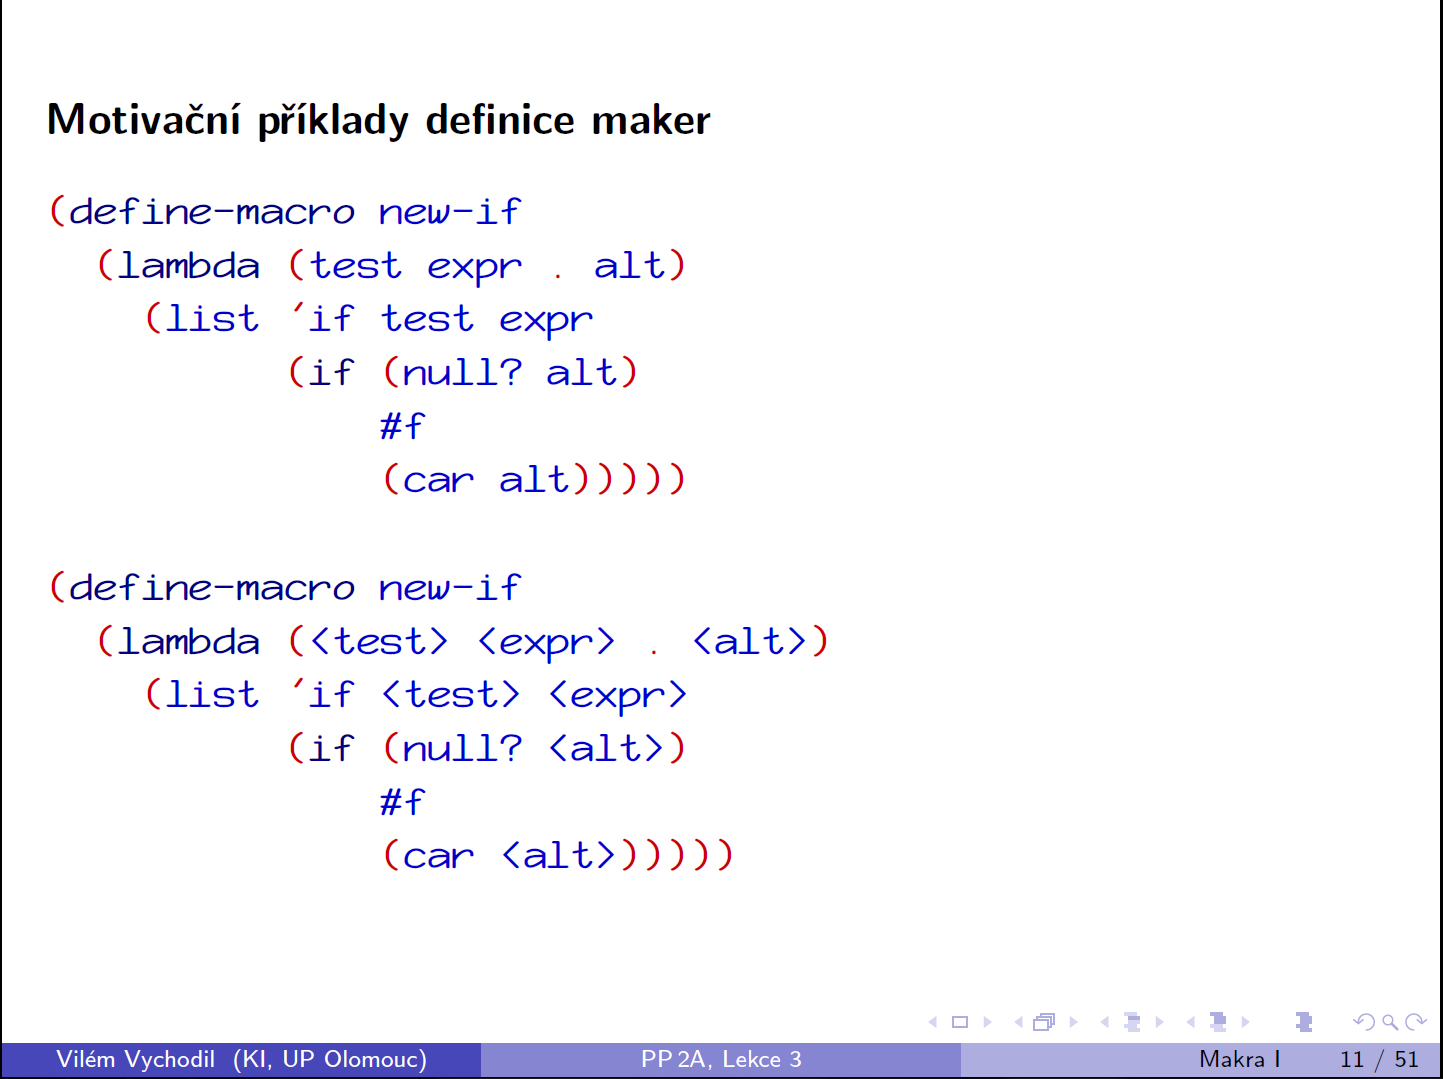
\includegraphics[scale=0.25]{img/makra_normalni_pouziti_1}
	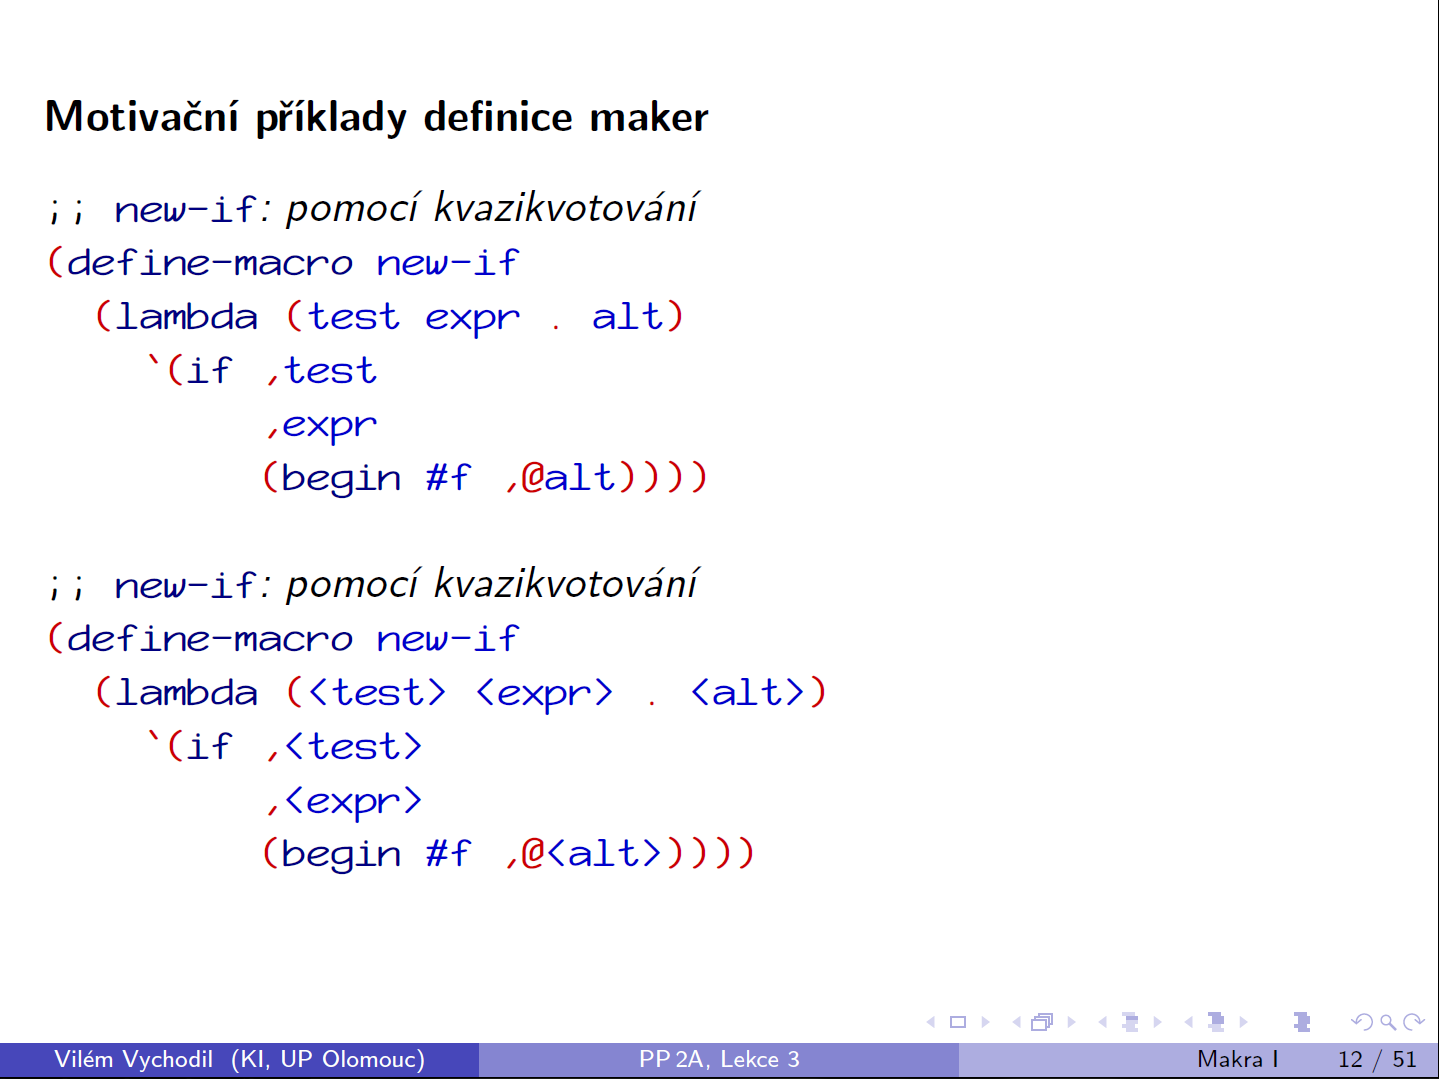
\includegraphics[scale=0.25]{img/makra_normalni_pouziti_2}
	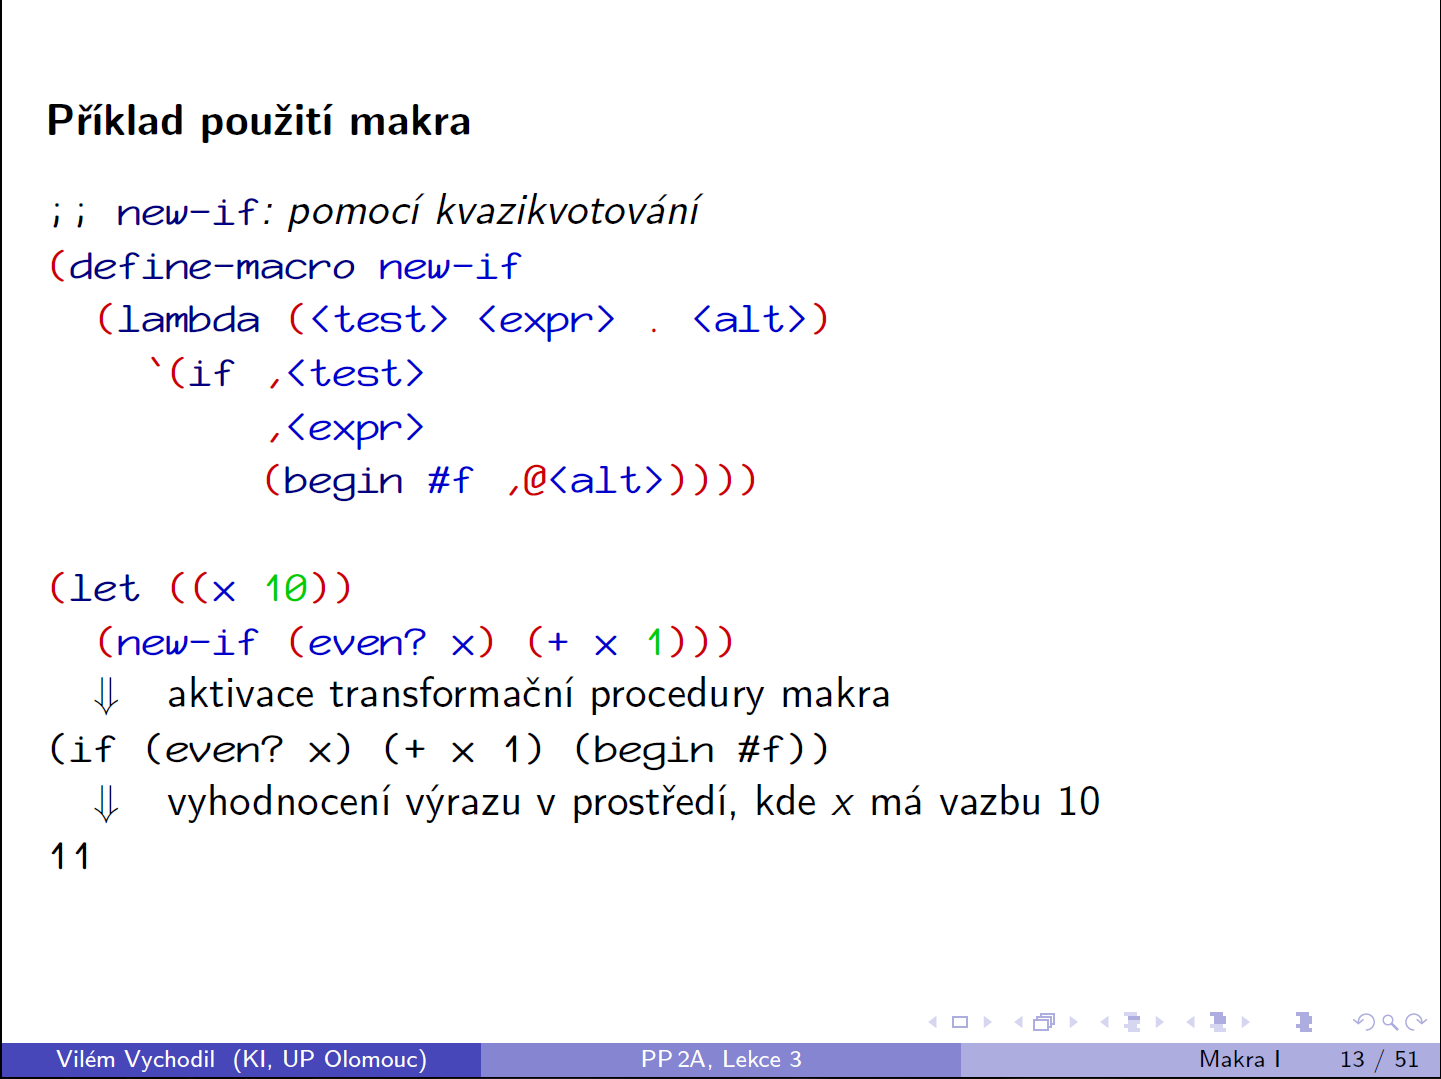
\includegraphics[scale=0.25]{img/makra_normalni_pouziti_3}
\end{center}

\subsubsection{Hygienická makra}
\begin{center}
	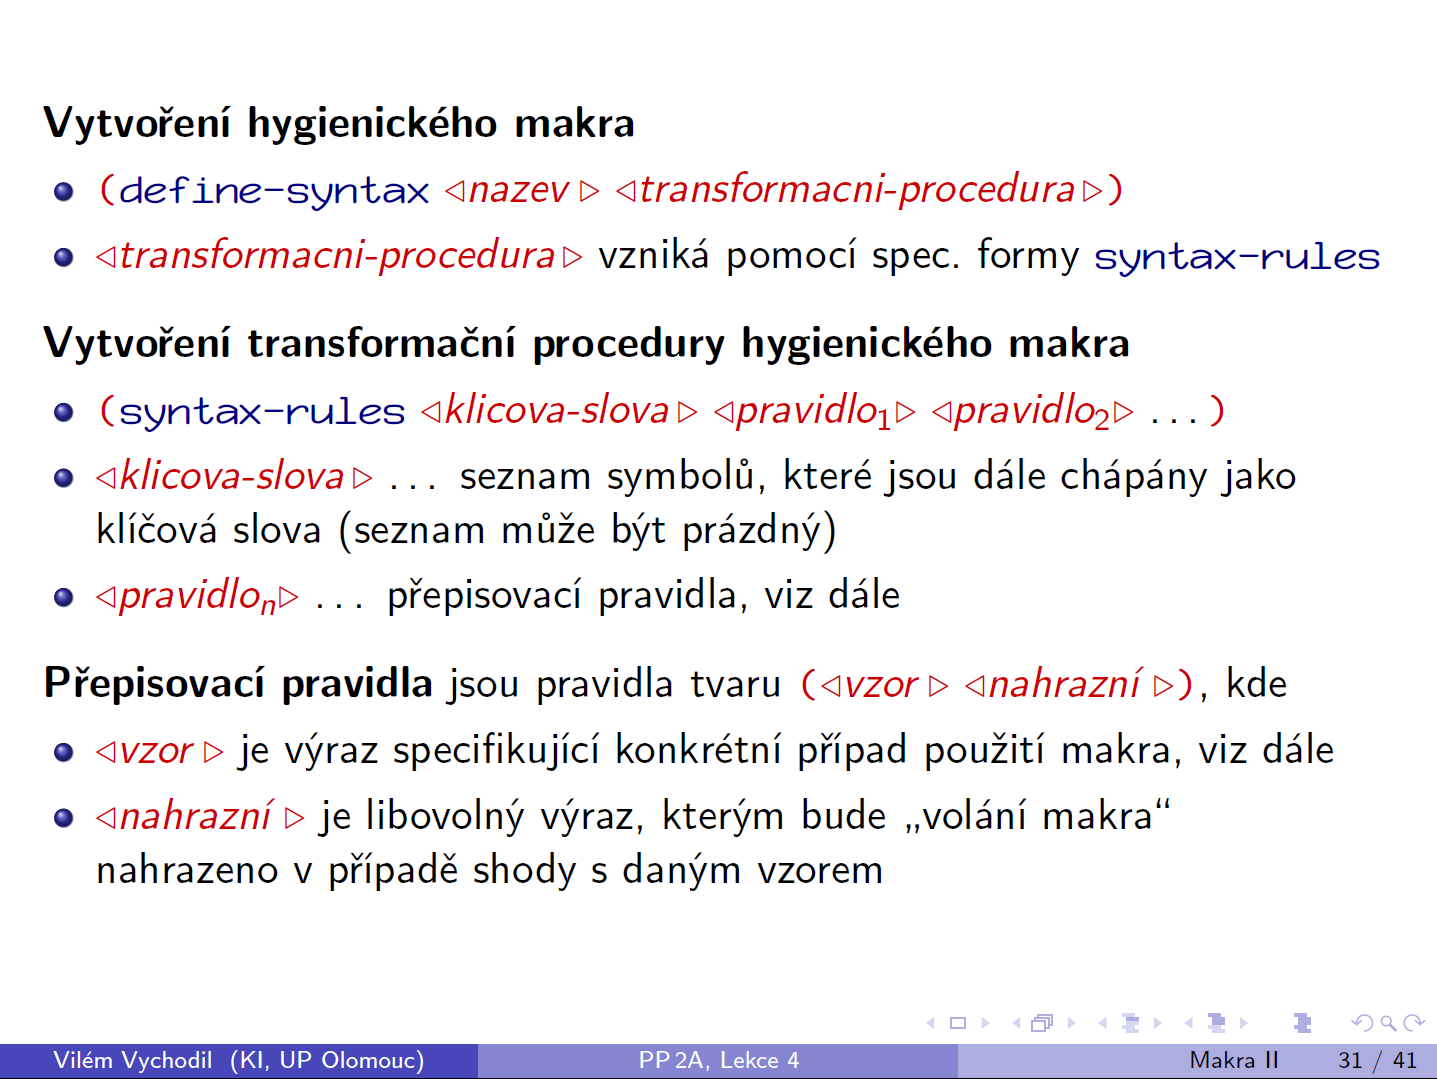
\includegraphics[scale=0.35]{img/makra_hygienicka_pouziti_1}
	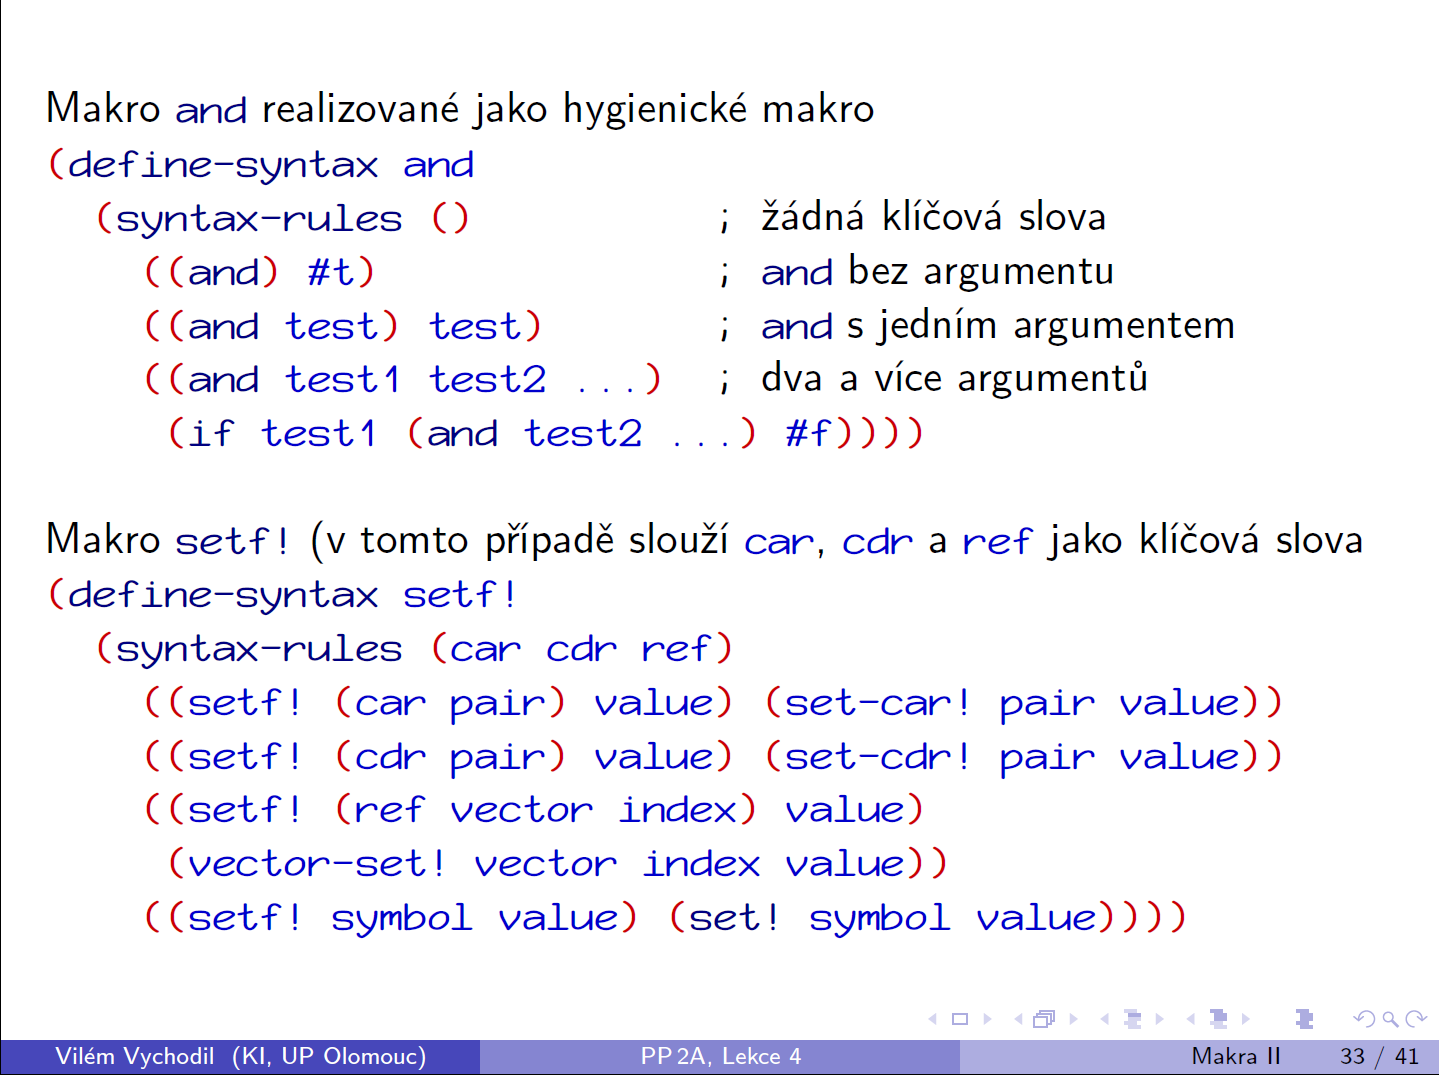
\includegraphics[scale=0.35]{img/makra_hygienicka_pouziti_2}
\end{center}

\section{Líné vyhodnocování, přísliby a proudy}
\subsection{Přísliby a líne vyhodnocování}
Základní myšlenka:
\begin{itemize}
	\item místo vyhodnocení daného výrazu pracujeme s \textit{příslibem} jeho budoucího vyhodnocení
	\item \textit{příslib} = nový typ elementu (element prvního řádu
	\item speciální forma \color{blue} delay \color{black}, která pro daný výraz vrací příslib jeho vyhodnocení
	\item procedura \color{blue} force \color{black}, která pro daný příslib aktivuje výpočet a vrátí hodnotu vzniklou vyhodnocením přislíbeného výrazu
\end{itemize}
Líné vyhodnocování = vyhodnocování založené na příslibech (někdy taky "call by need")
\paragraph{Poznámka.}
\begin{itemize}
	\item Při líném vyhodnocování dochází k propagaci chyb (chyba se projeví "na jiném místě" než "kde vznikla".
	\item pomocí příslibů je možné "odložit časově složitý výpočet na později" a aktivovat jej, až je skutečně potřeba jej provést.
\end{itemize}

\subsection{Proudy (Streams)}
\begin{itemize}
	\item proudy jsou nejčastěji používanou aplikací líného vyhodnocování
	\item neformálně: proudy jsou líně vyhodnocované seznamy
	\item konstruktor \textit{cons-stream} a selektory \textit{stream-car} a \textit{stream-cdr}
	\item prázdný seznam je proud
	\item každý tečkový pár (\textit{e} . \textit{p}), kde \textit{e} je libovolný element a \textit{p} je příslib proudu, je proud.
	\item výpočet je řízen daty, dochází k propagaci chyb
\end{itemize}
\begin{center}
	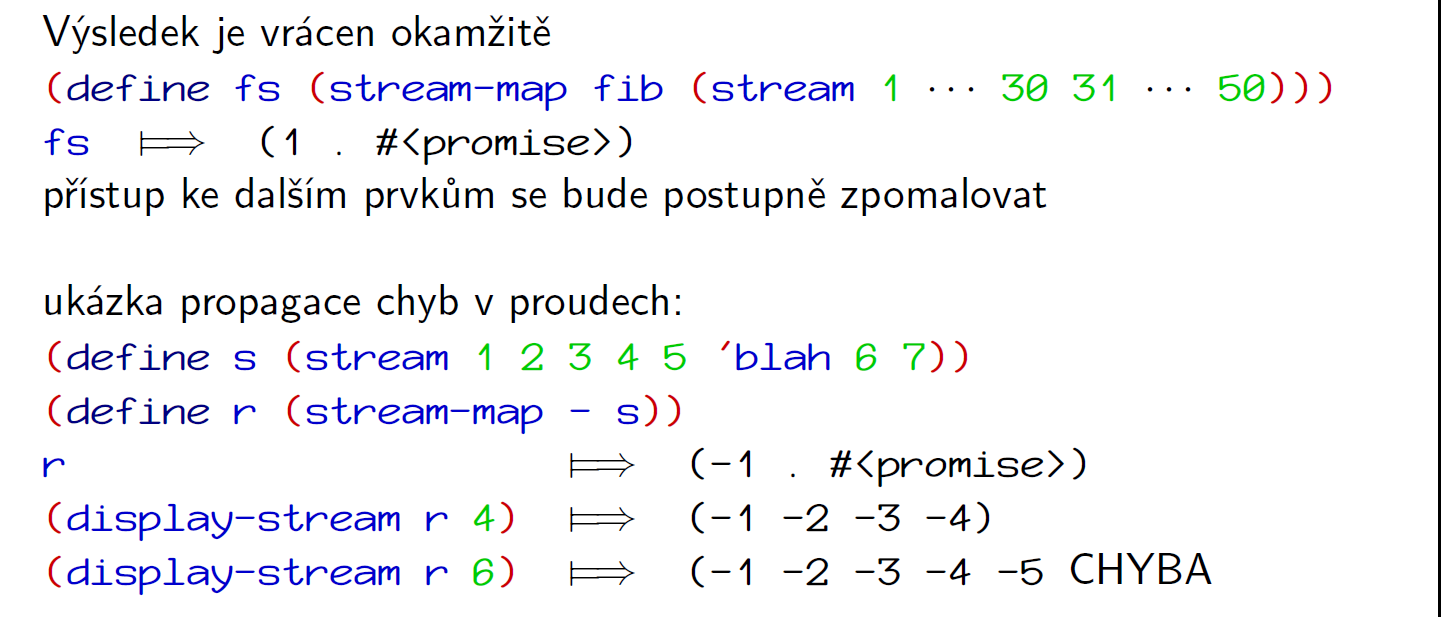
\includegraphics[scale=0.35]{img/streams_1}
\end{center}

\subsubsection{Nekonečné proudy}
\begin{itemize}
	\item neformálně: "potenciálně nekonečná lineární datová struktura"
	\item v každém okamžiku průchodu nekonečným proudem máme vždy k dispozici aktuální prvek a příslib
	\item v praxi se konstruuje rekurzivní procedurou bez limitní podmínky
\end{itemize}
\begin{center}
	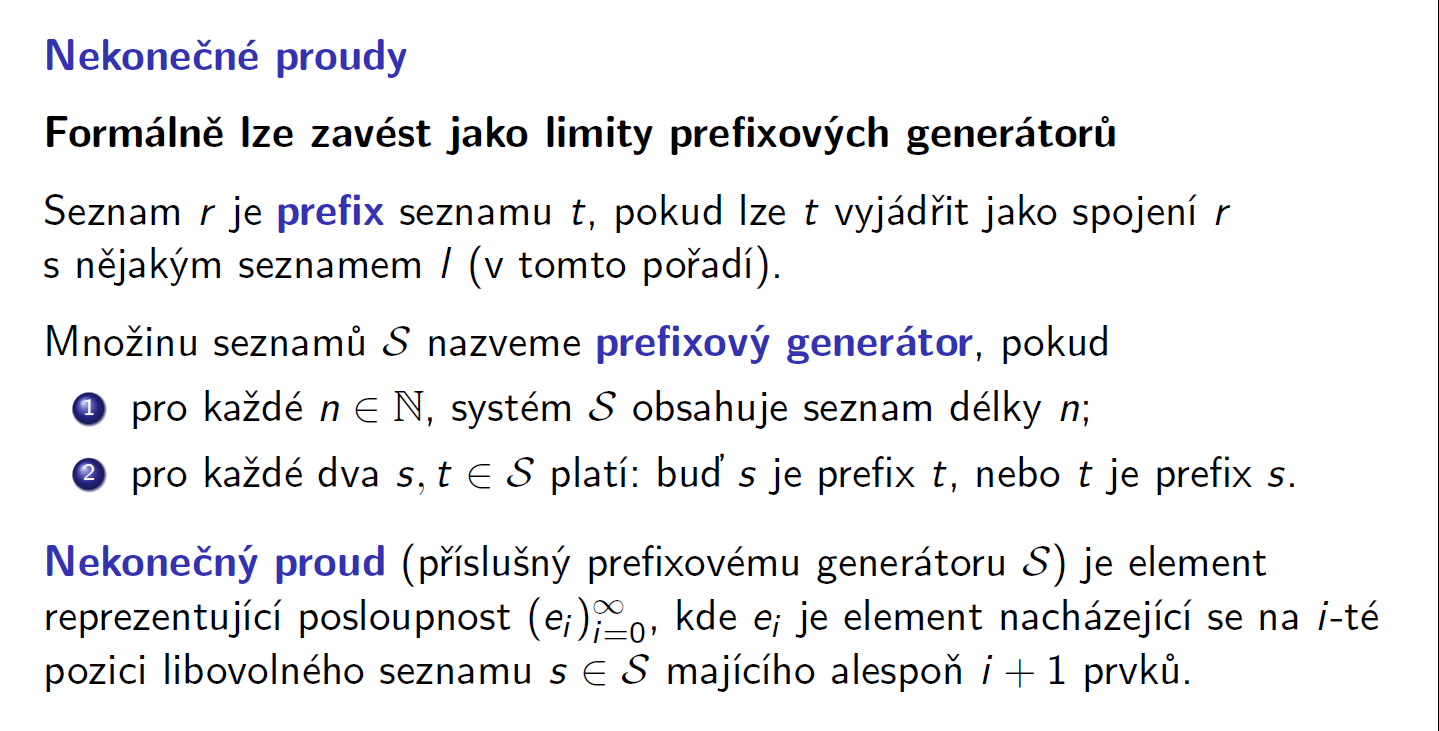
\includegraphics[scale=0.35]{img/nekonecne_proudy_1}
	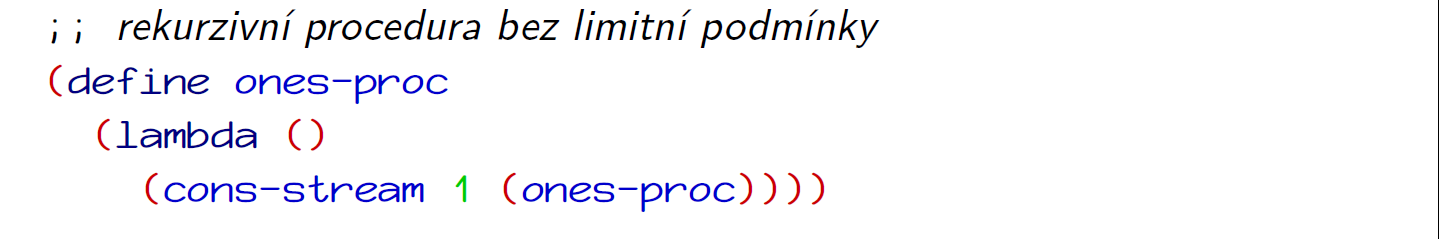
\includegraphics[scale=0.35]{img/nekonecne_proudy_2}
	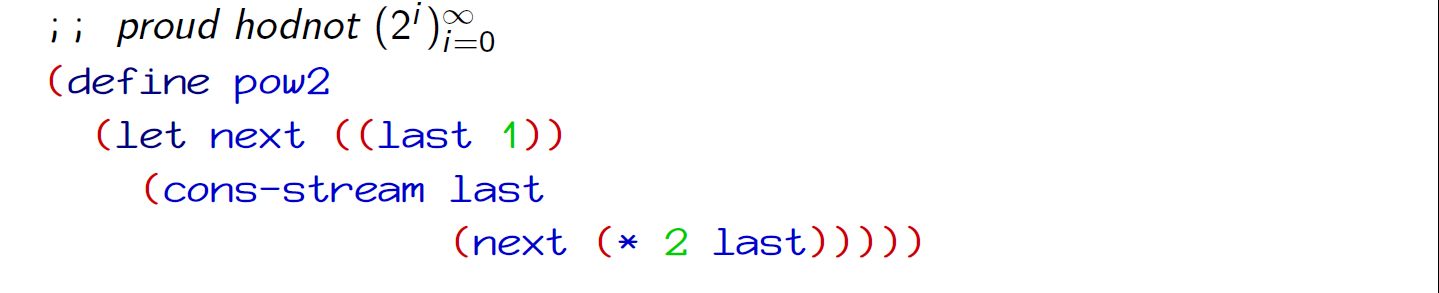
\includegraphics[scale=0.35]{img/nekonecne_proudy_3}
\end{center}

\newpage
\section{Aktuální pokračování a únikové funkce}
\begin{center}
	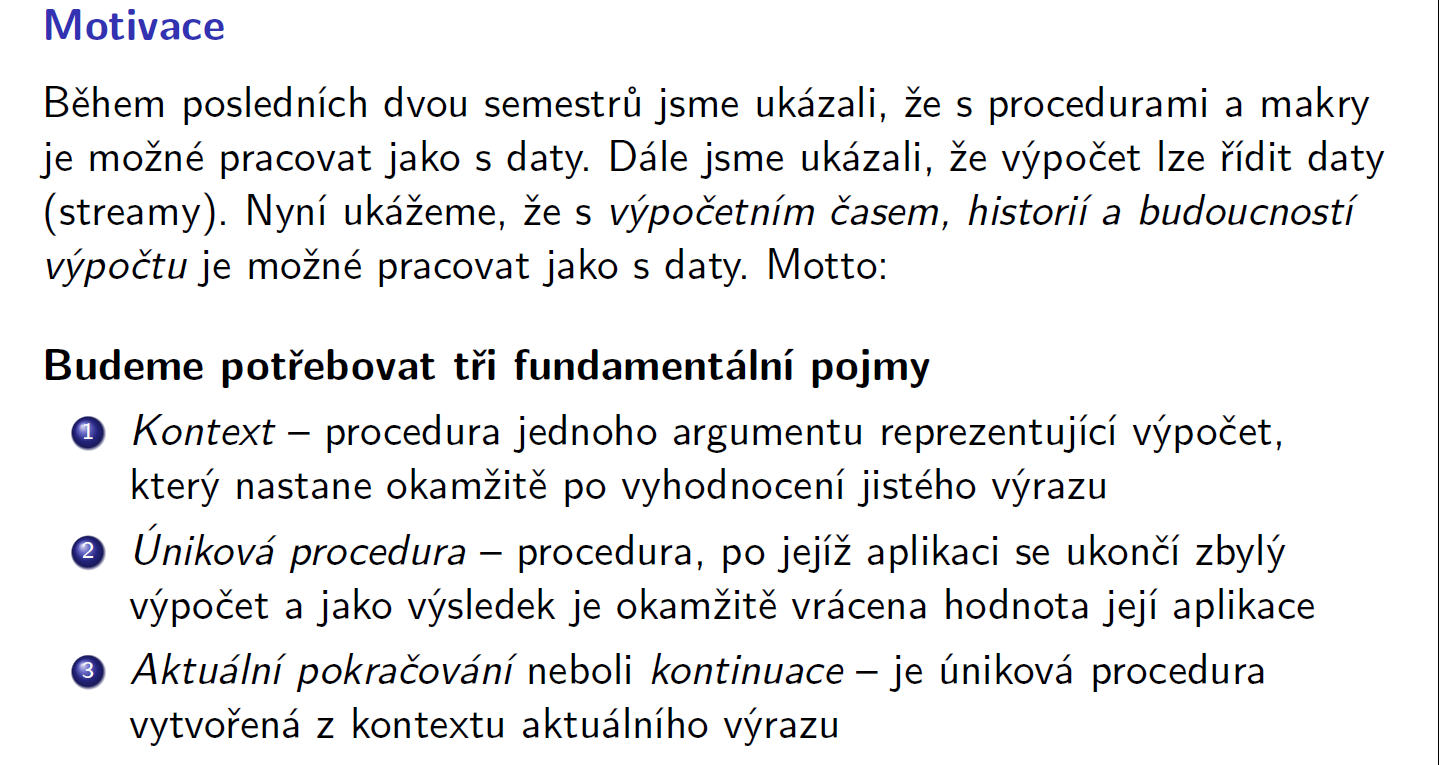
\includegraphics[scale=0.35]{img/aktualni_pokracovani_1}
	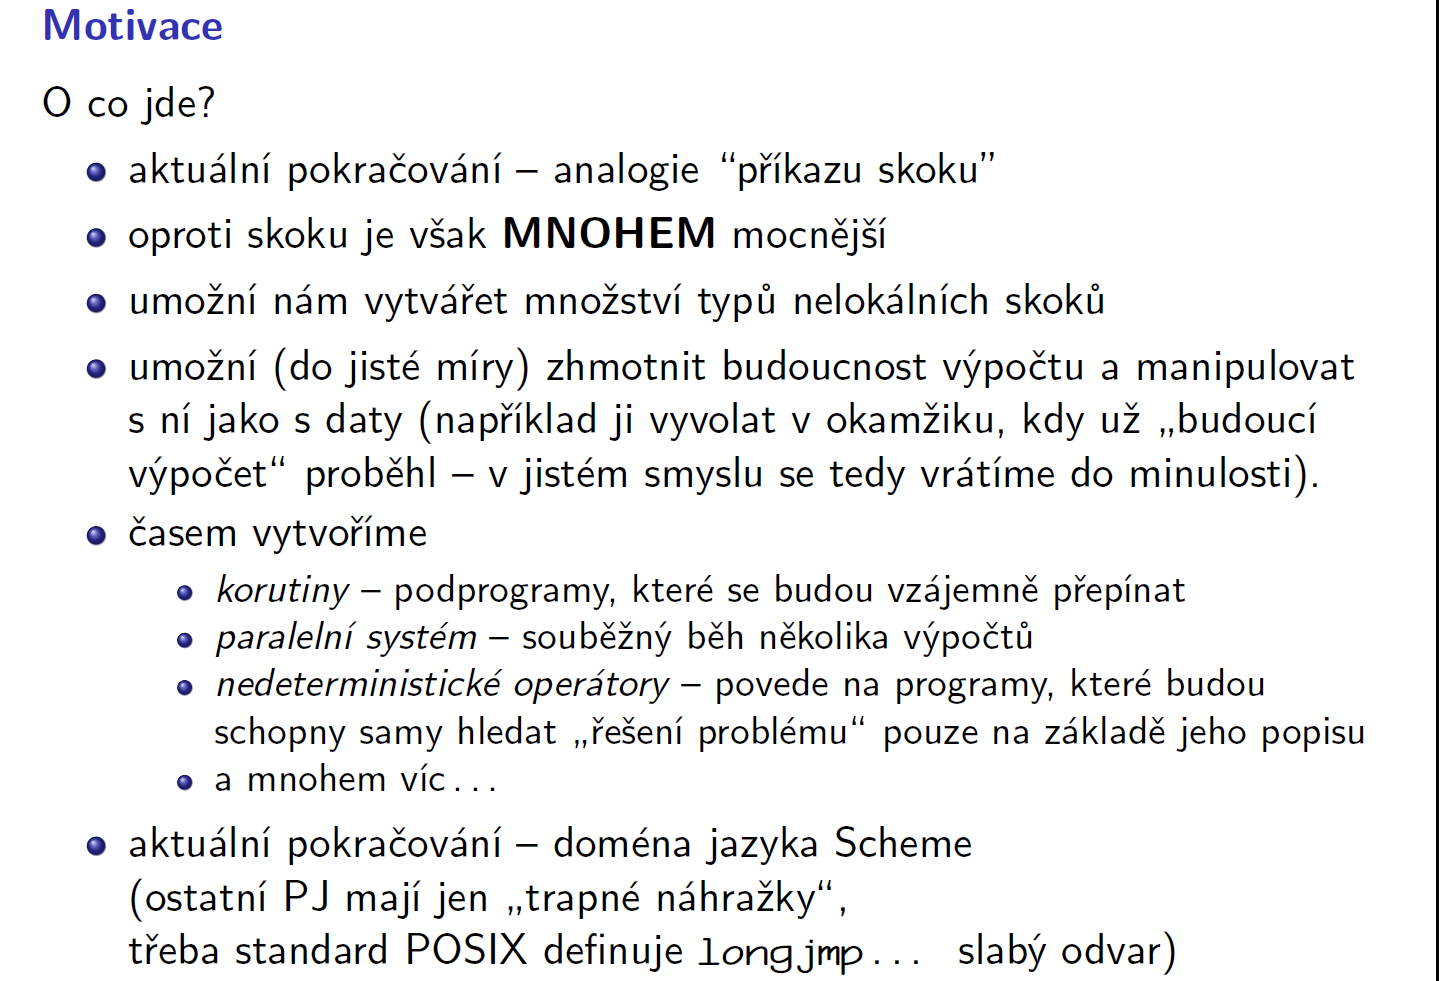
\includegraphics[scale=0.35]{img/aktualni_pokracovani_2}
	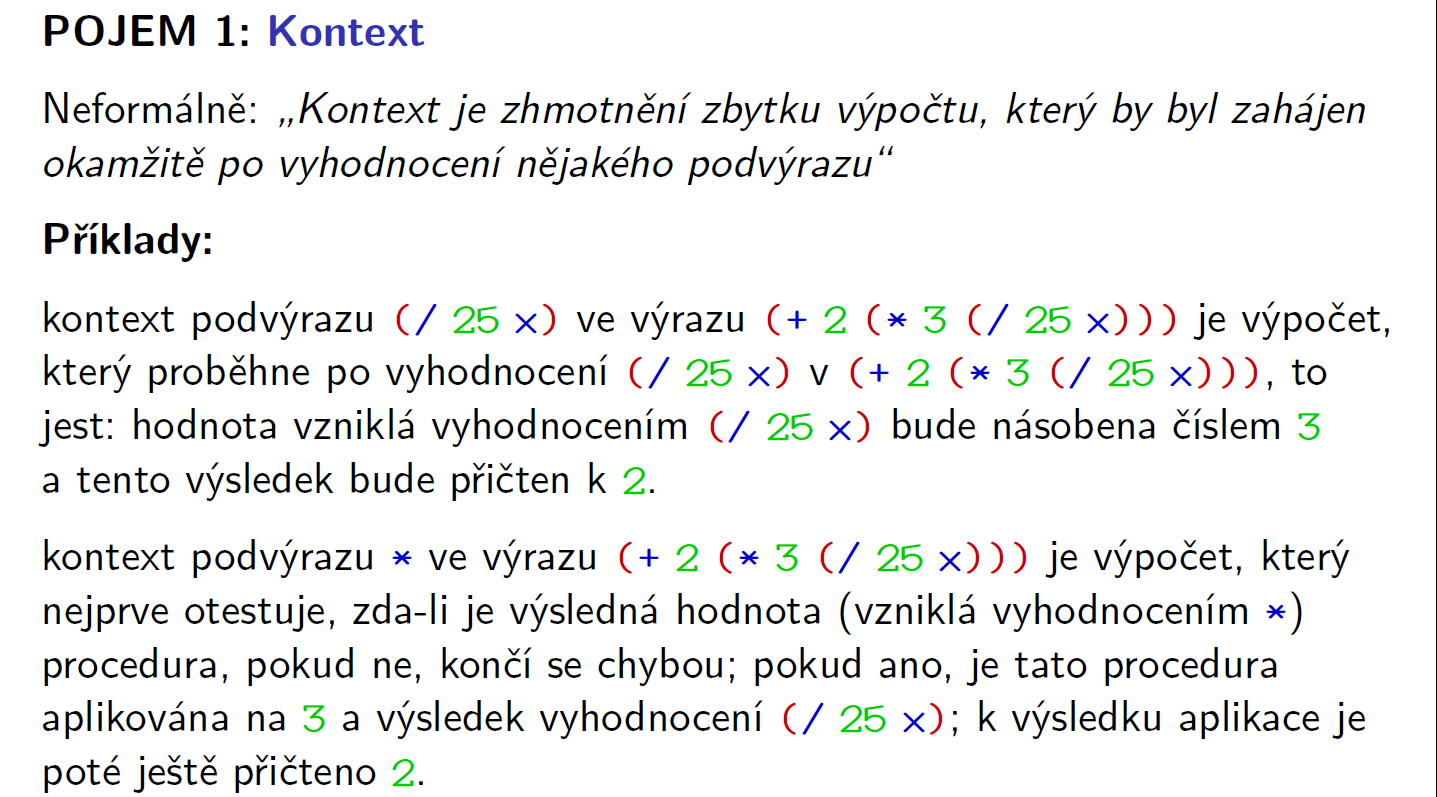
\includegraphics[scale=0.35]{img/aktualni_pokracovani_3}
	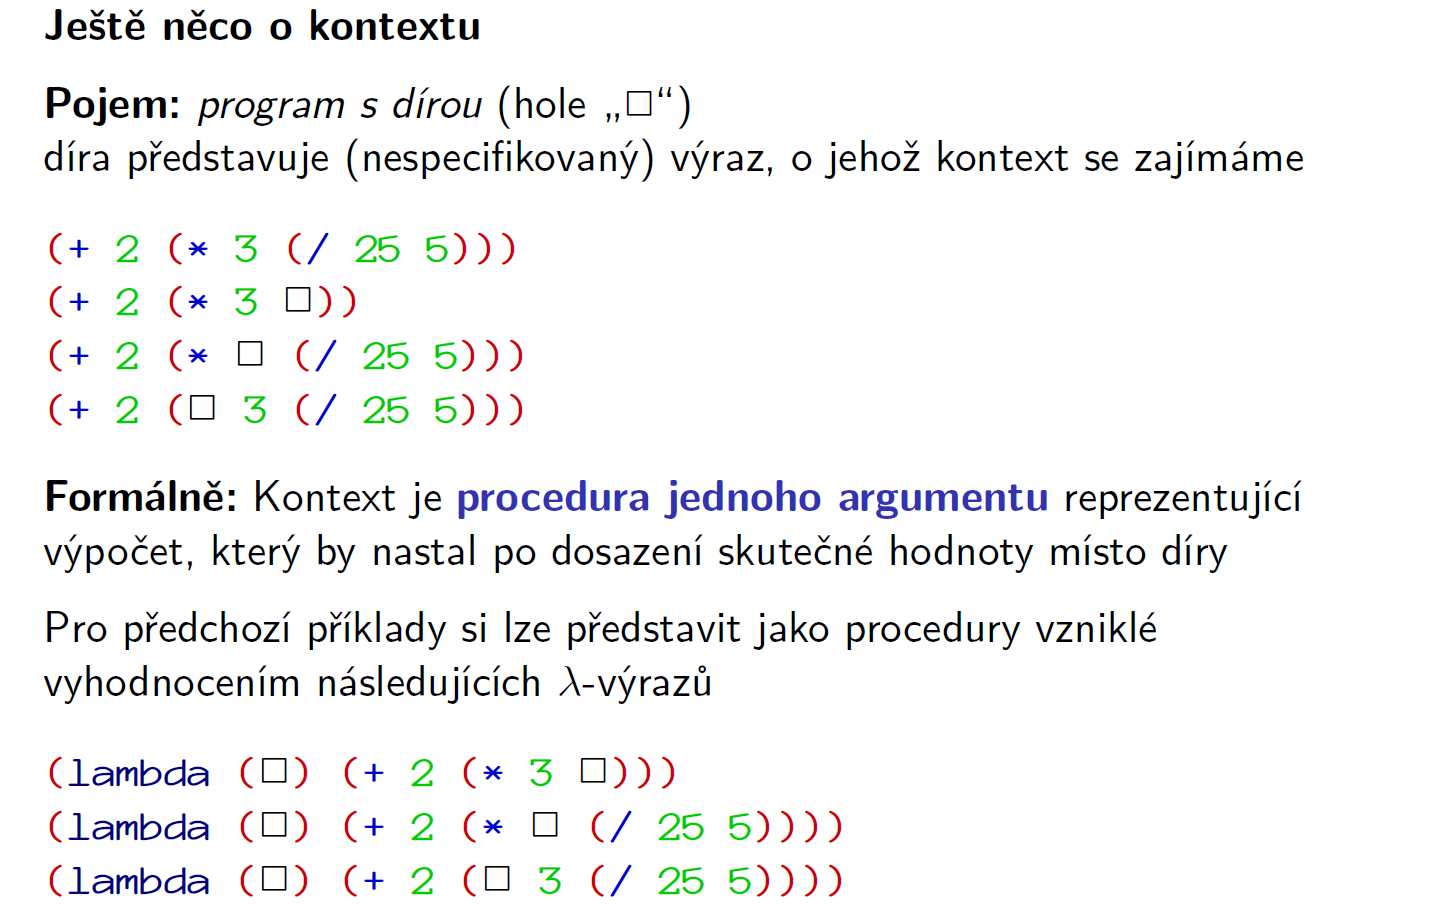
\includegraphics[scale=0.35]{img/aktualni_pokracovani_4}
	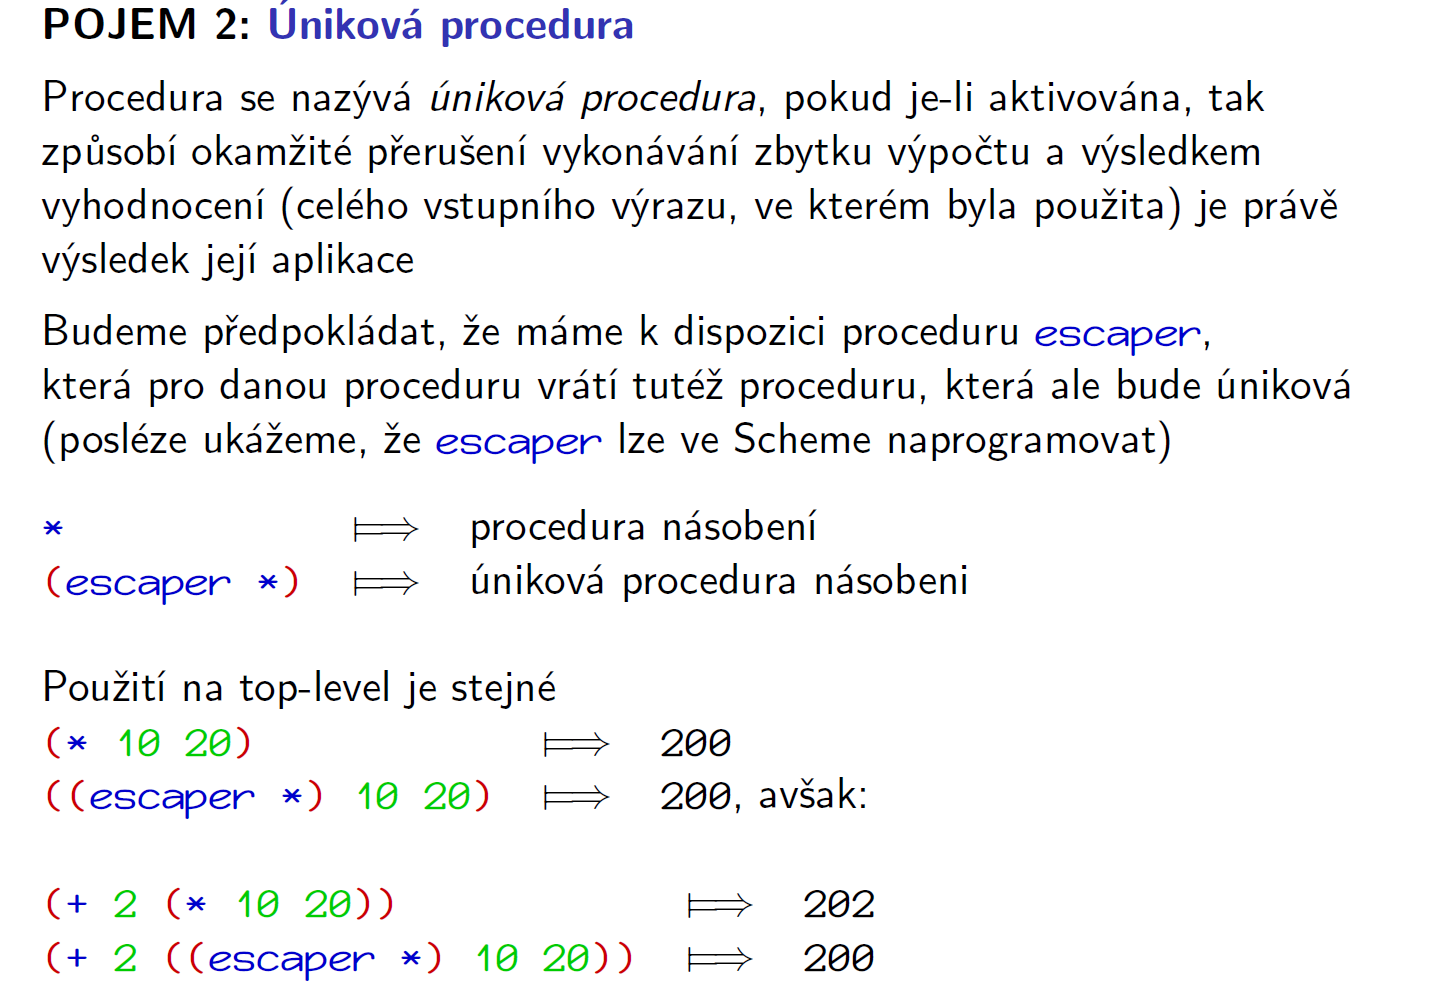
\includegraphics[scale=0.35]{img/aktualni_pokracovani_5}
	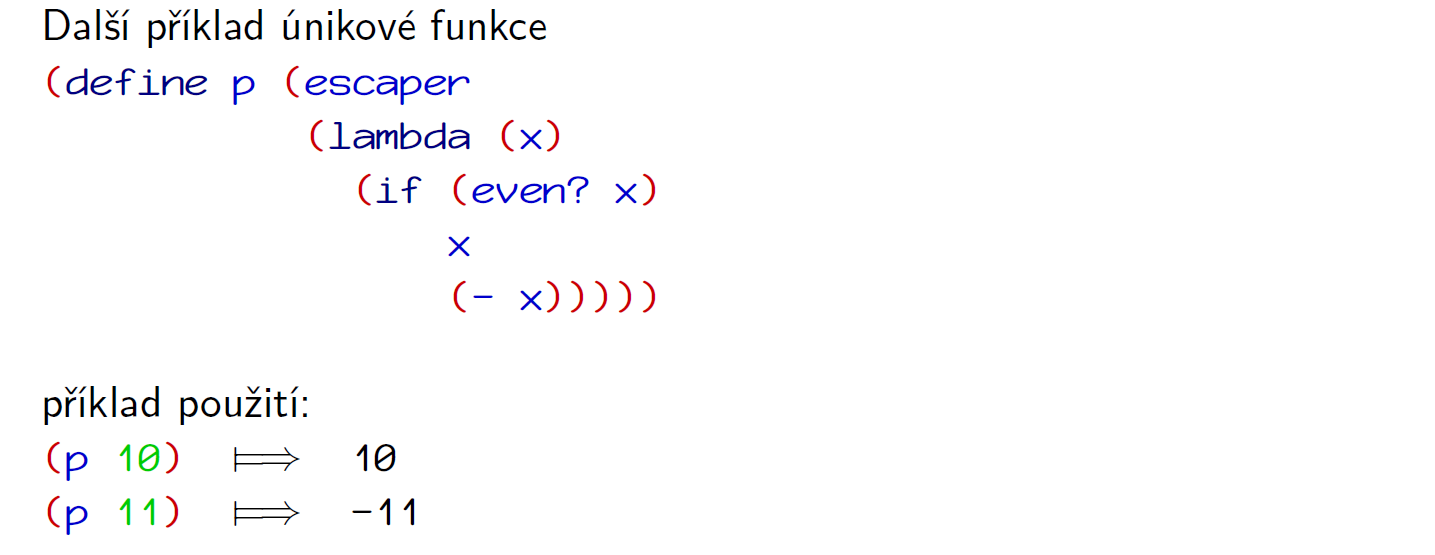
\includegraphics[scale=0.35]{img/aktualni_pokracovani_6}
	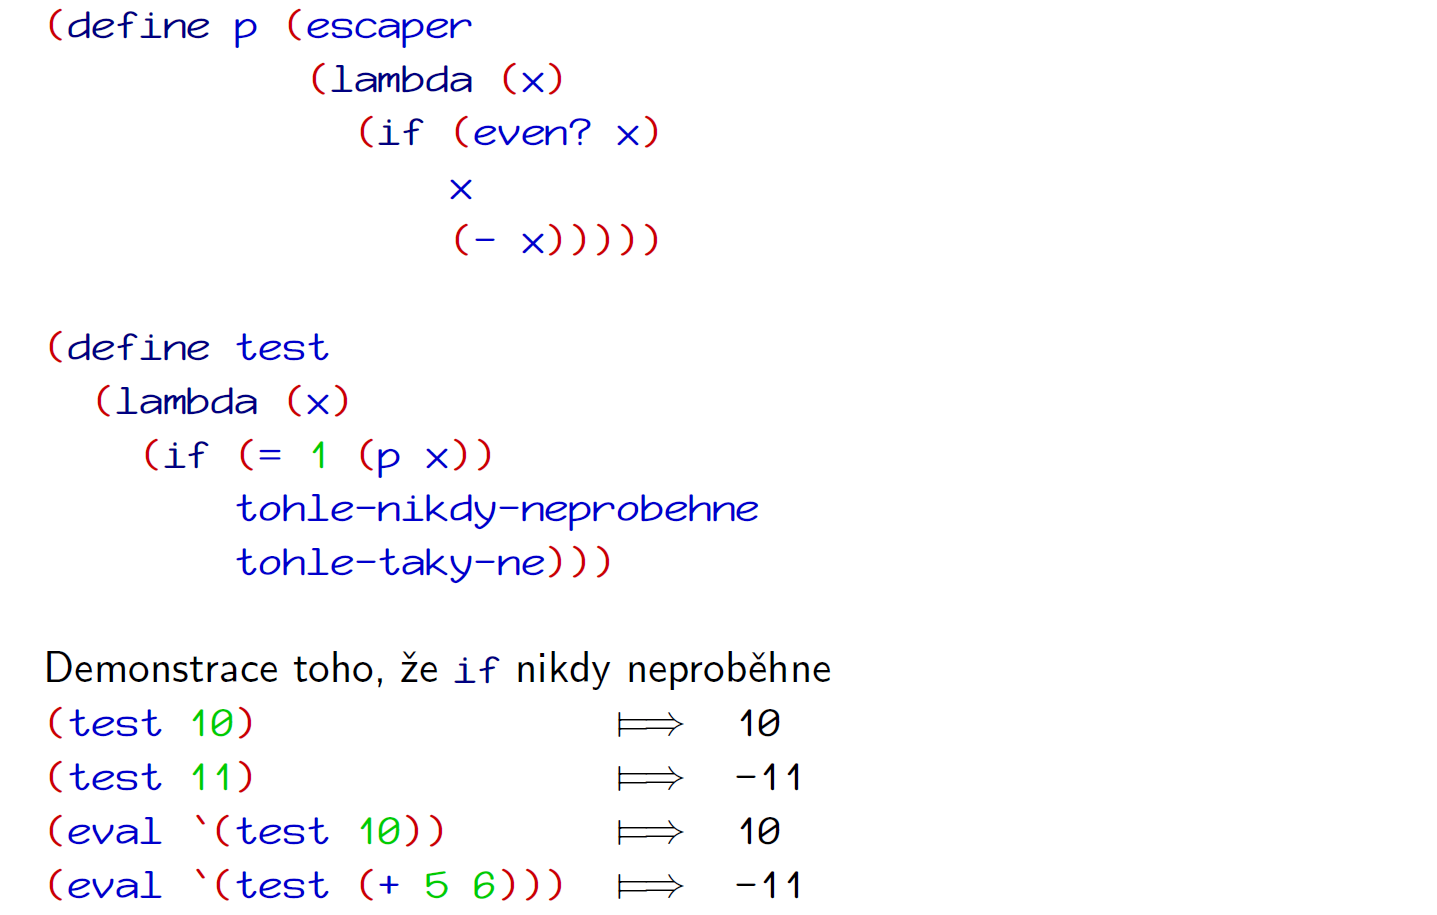
\includegraphics[scale=0.35]{img/aktualni_pokracovani_7}
	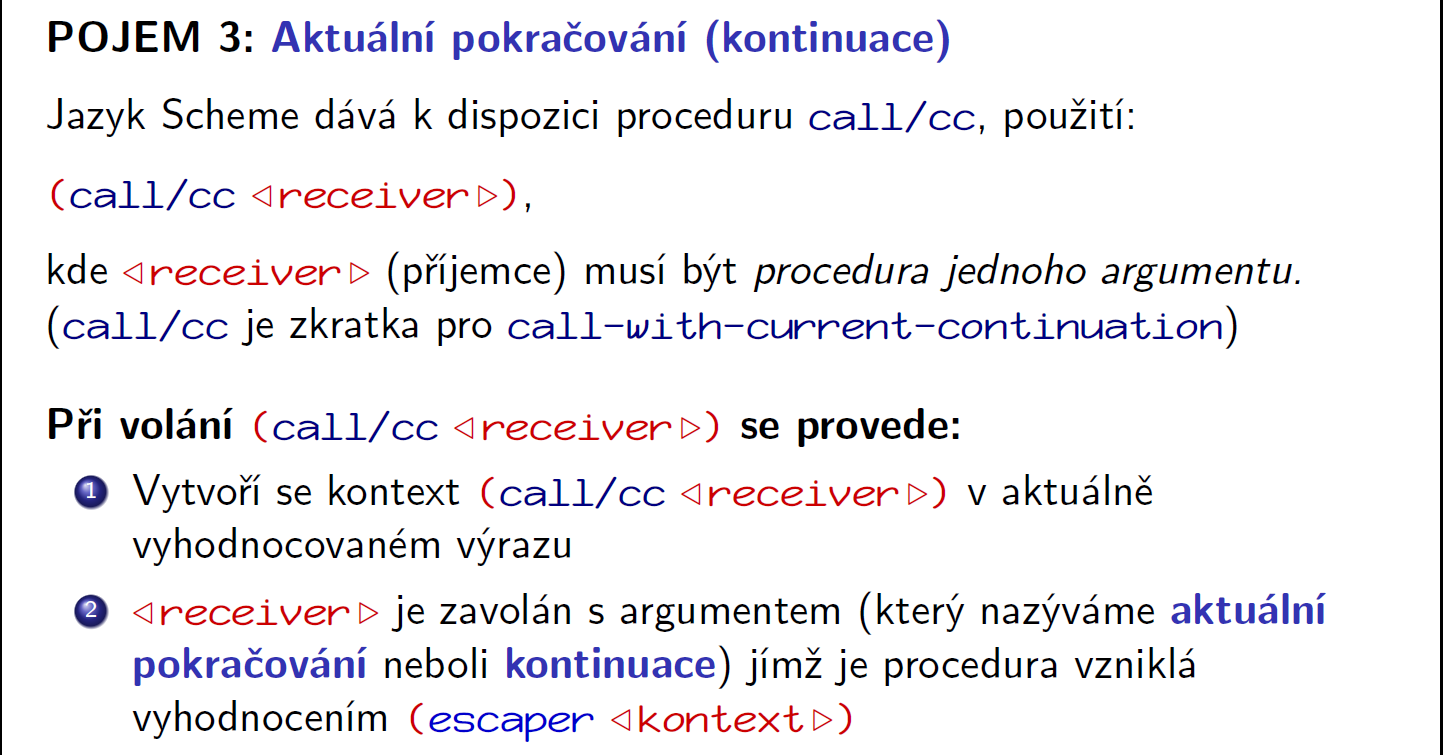
\includegraphics[scale=0.35]{img/aktualni_pokracovani_8}
	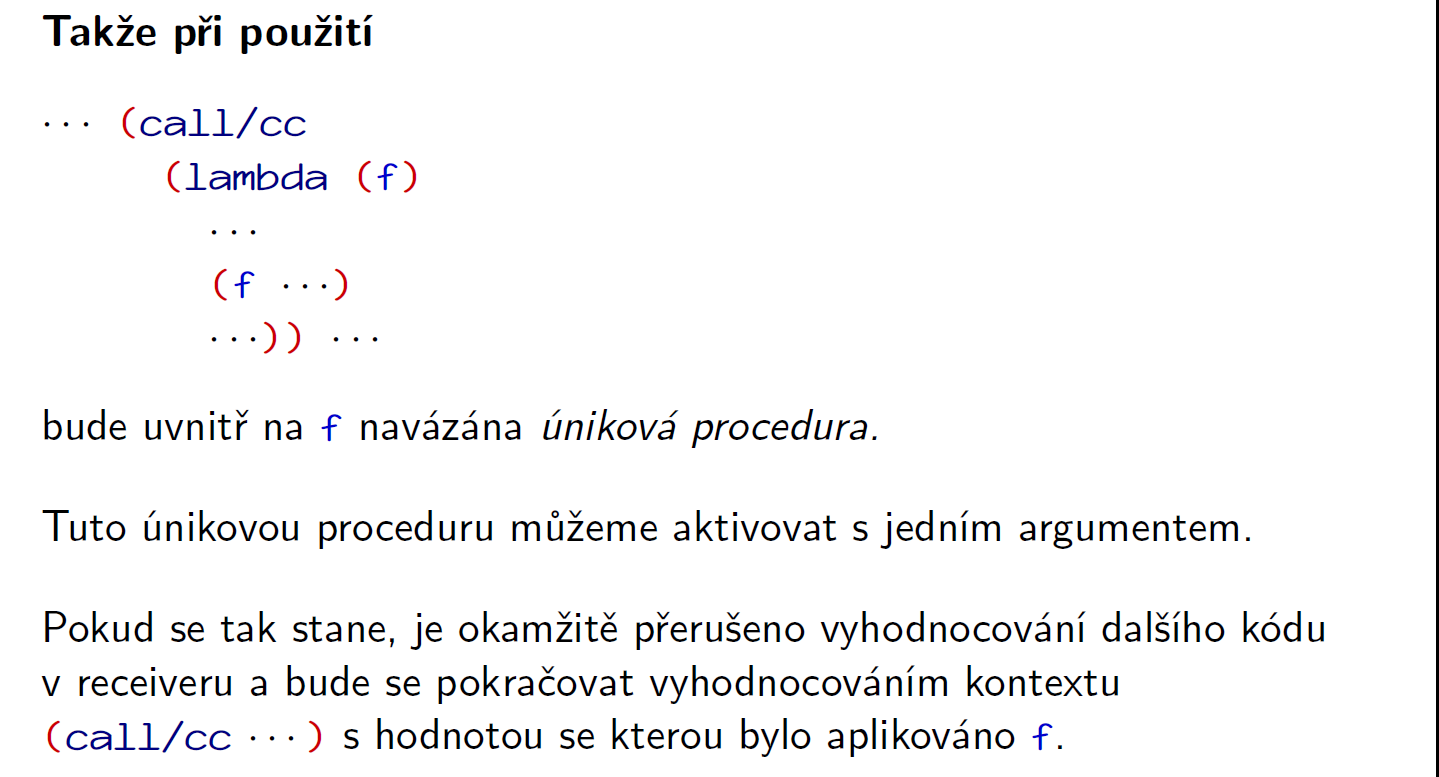
\includegraphics[scale=0.35]{img/aktualni_pokracovani_9}
	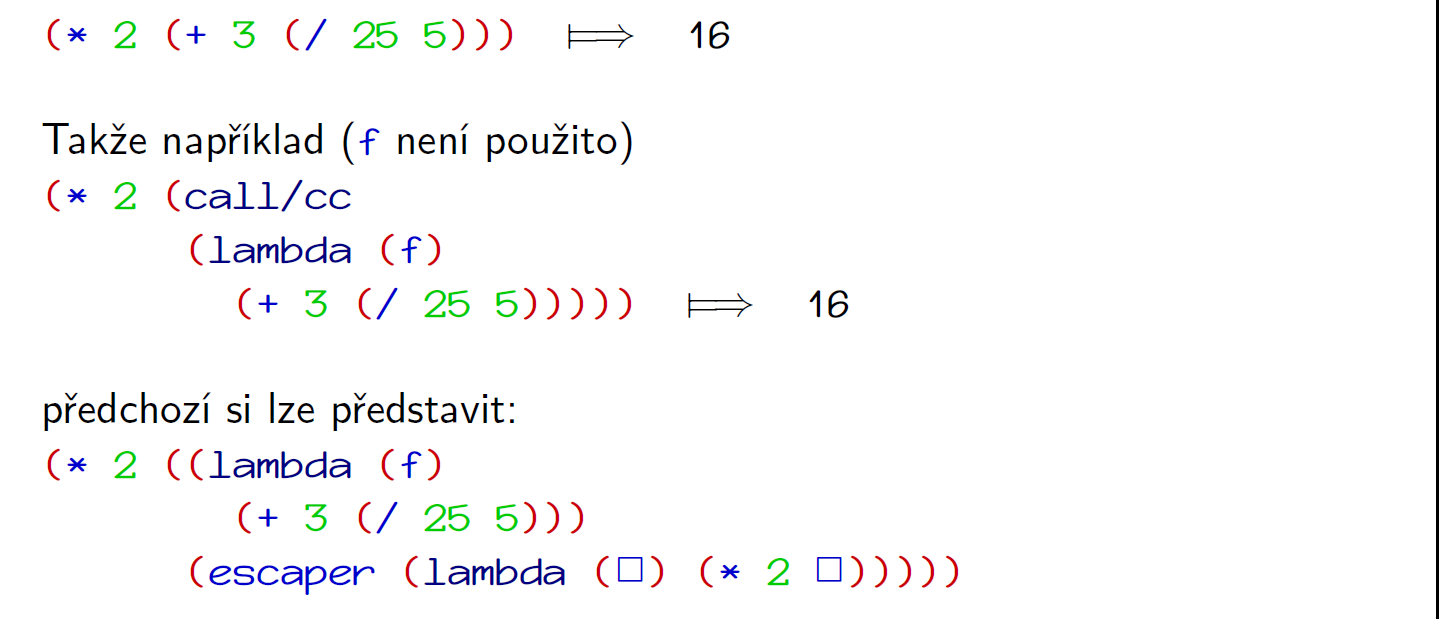
\includegraphics[scale=0.35]{img/aktualni_pokracovani_10}
	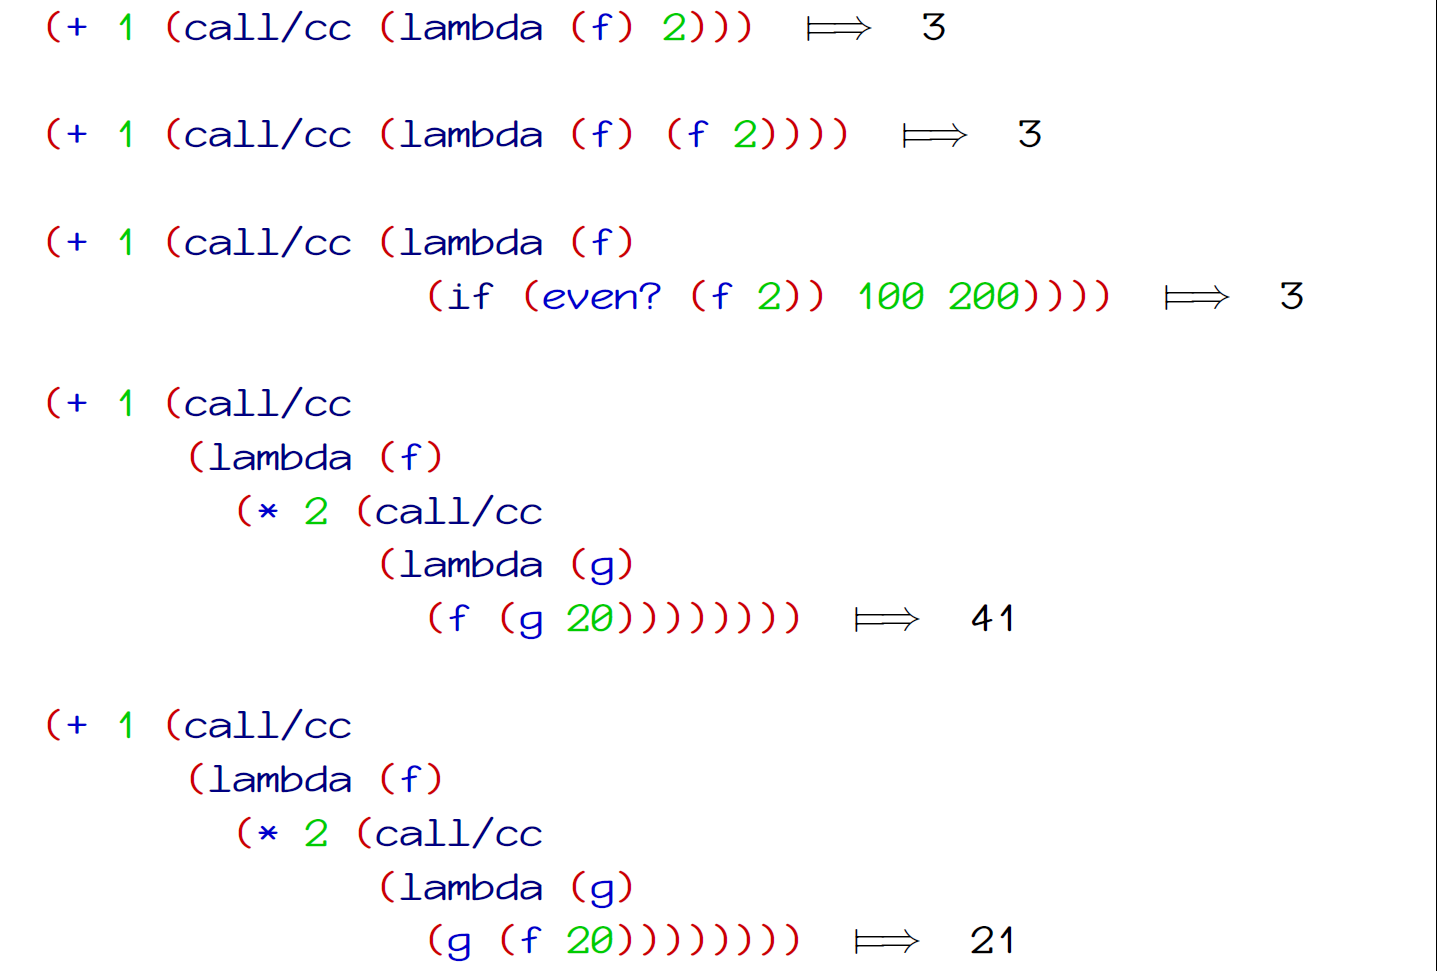
\includegraphics[scale=0.31]{img/aktualni_pokracovani_11}
	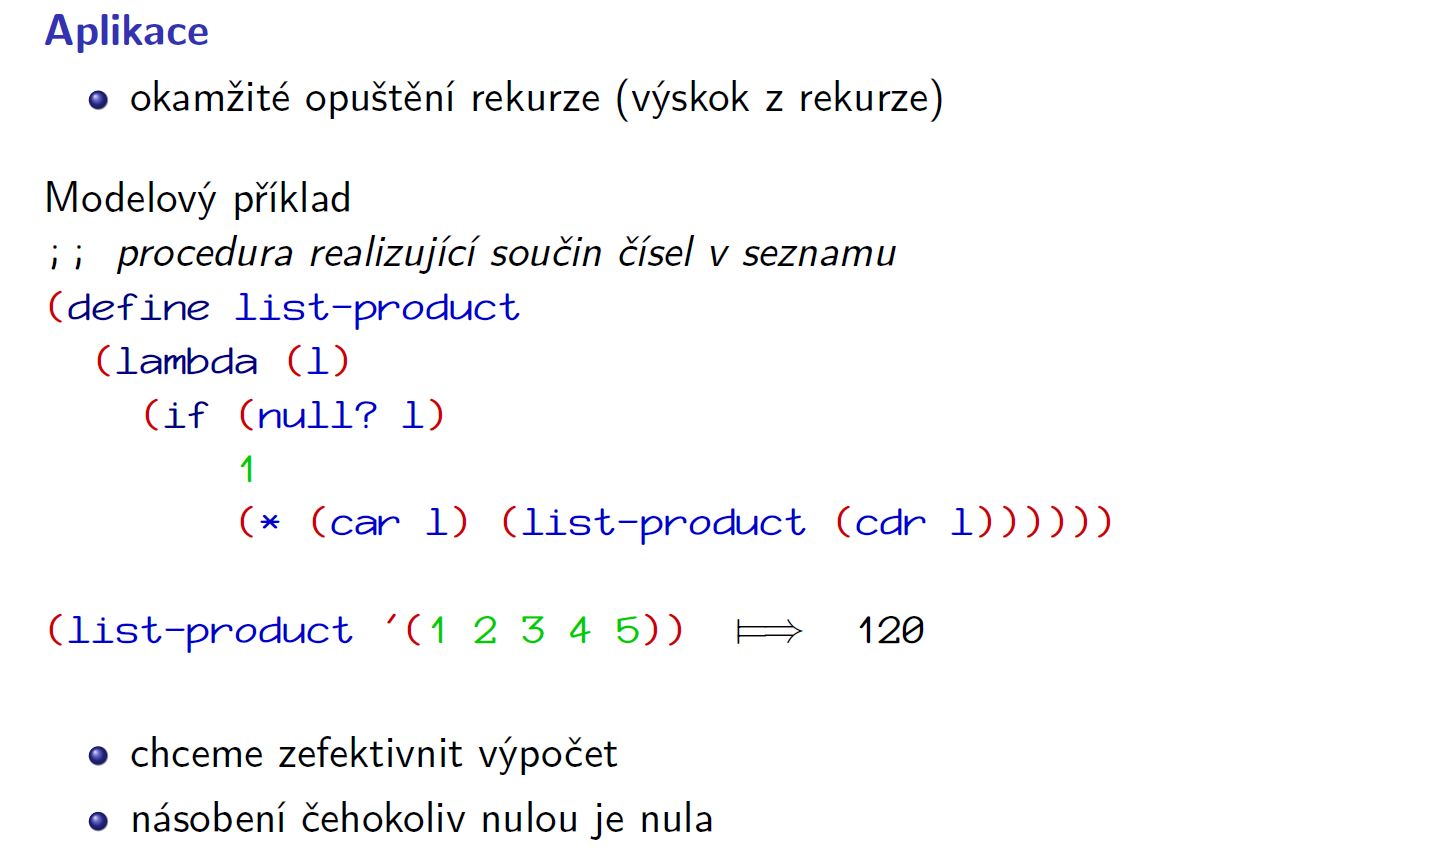
\includegraphics[scale=0.31]{img/aktualni_pokracovani_12}
	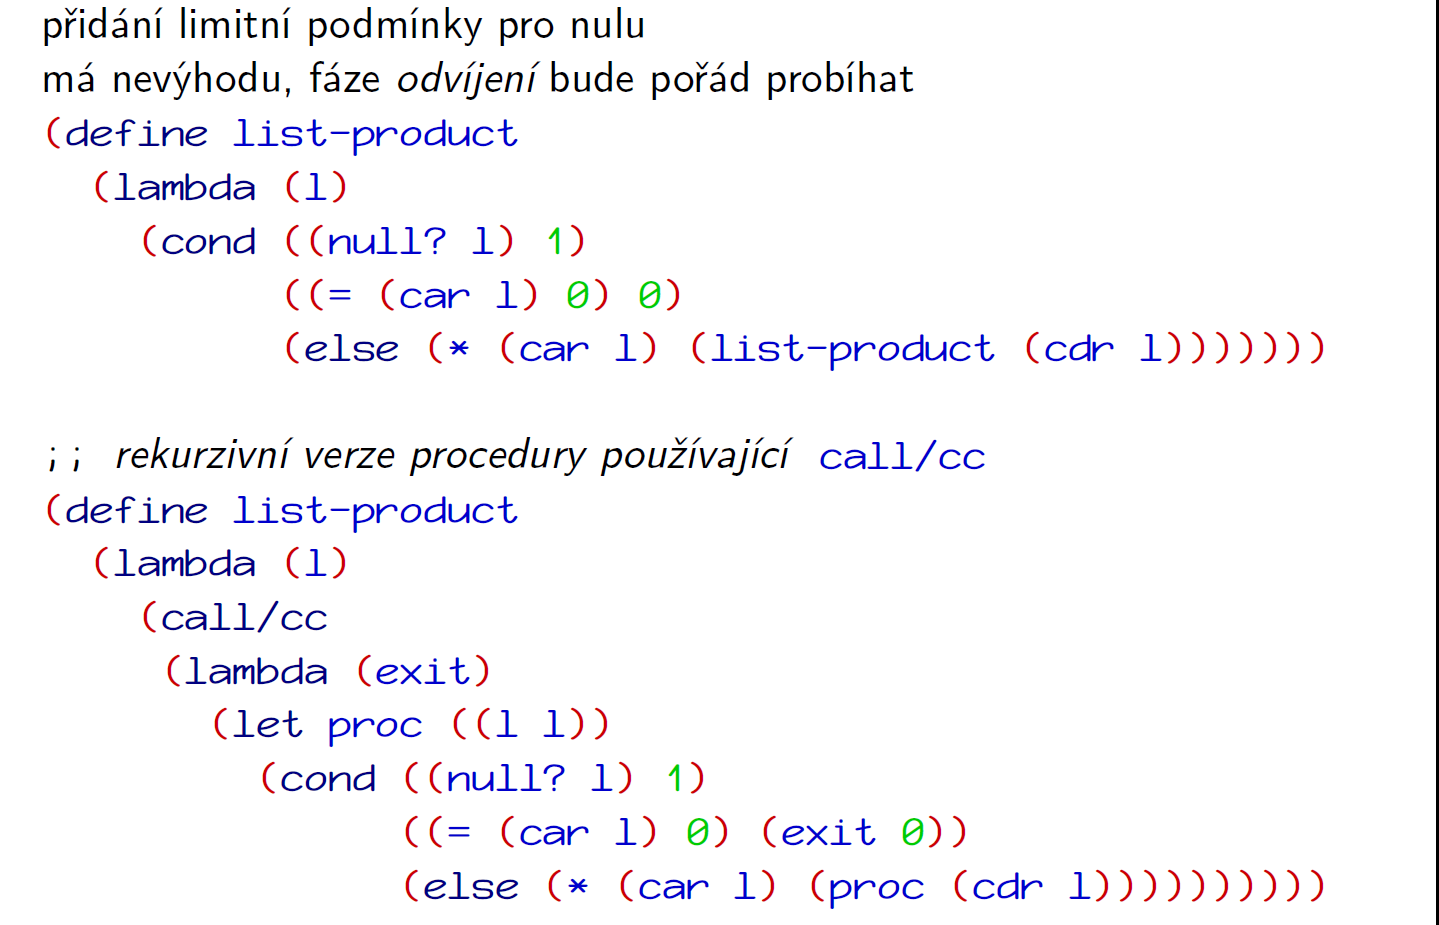
\includegraphics[scale=0.31]{img/aktualni_pokracovani_13}
\end{center}

\section{Zásobníkový model vyhodnocování programů (totálně nemám tušení co to je za hrůzu :D )}
\begin{center}
	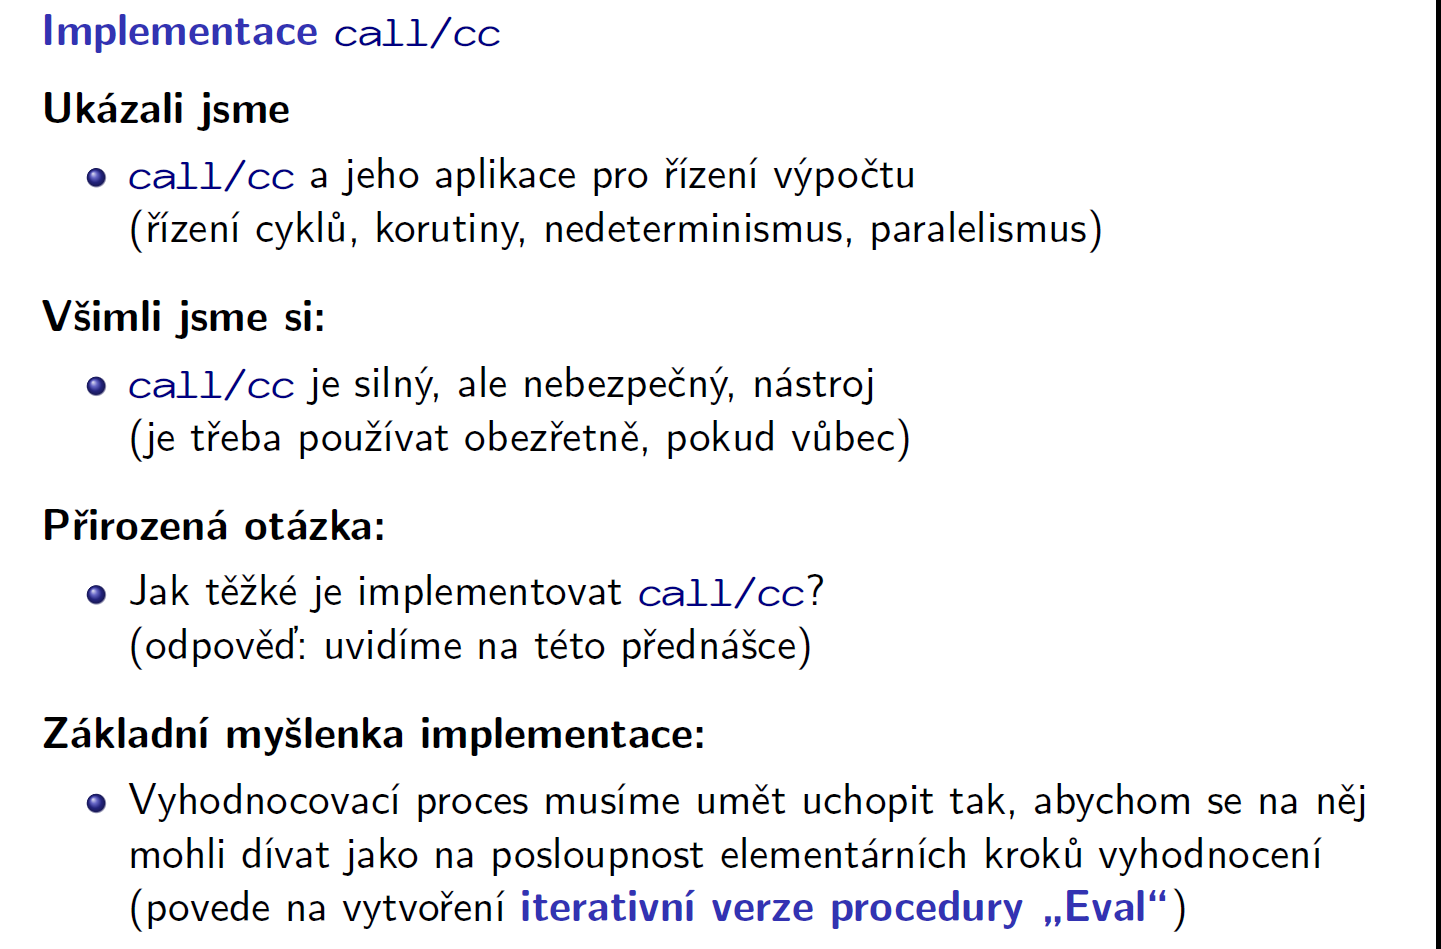
\includegraphics[scale=0.35]{img/zasobnikovy_model_1}
	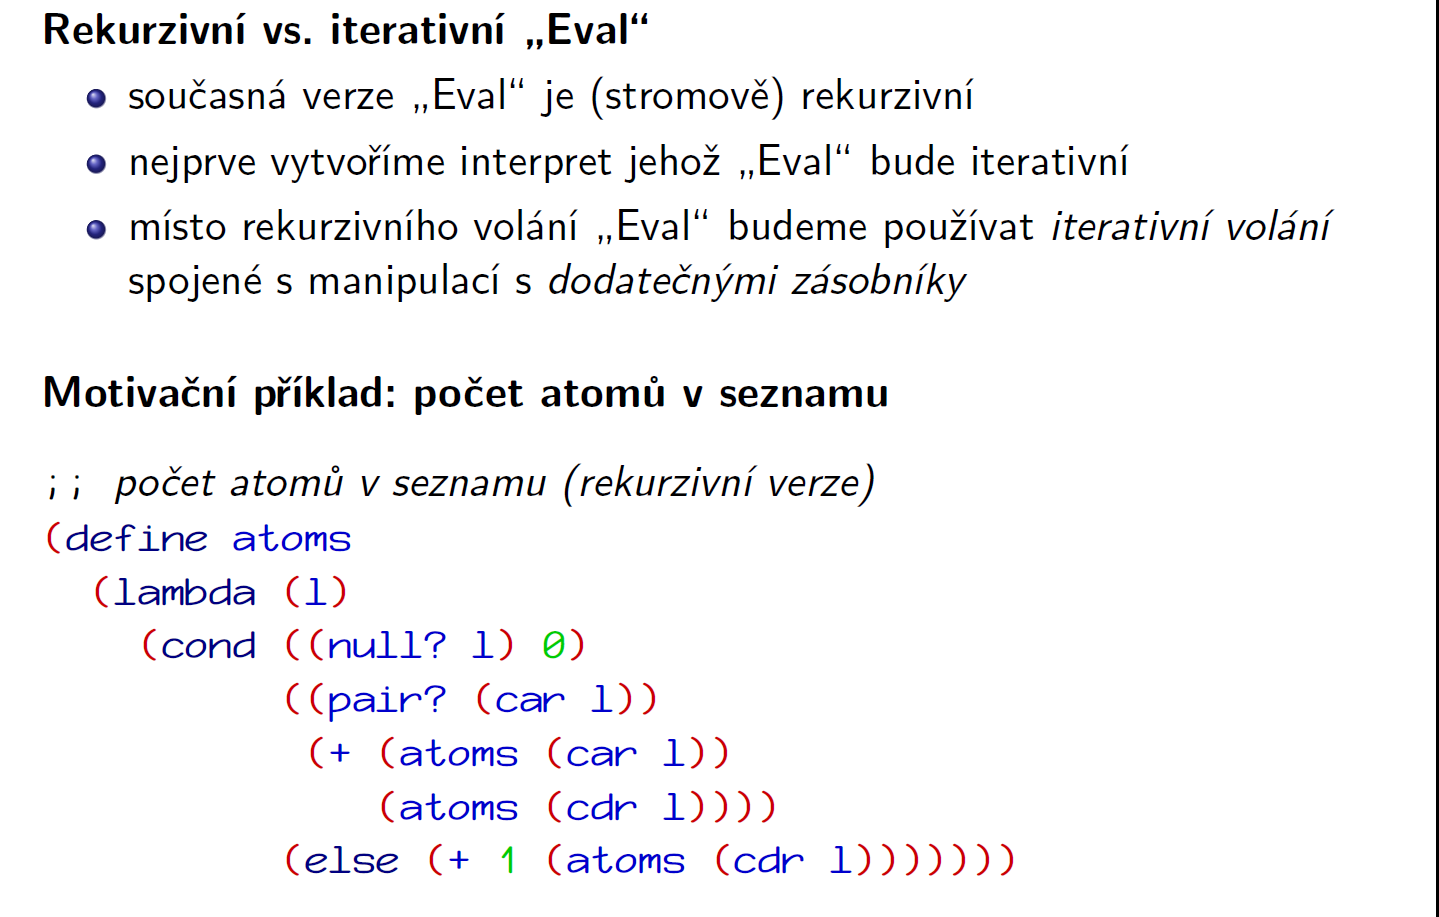
\includegraphics[scale=0.35]{img/zasobnikovy_model_2}
	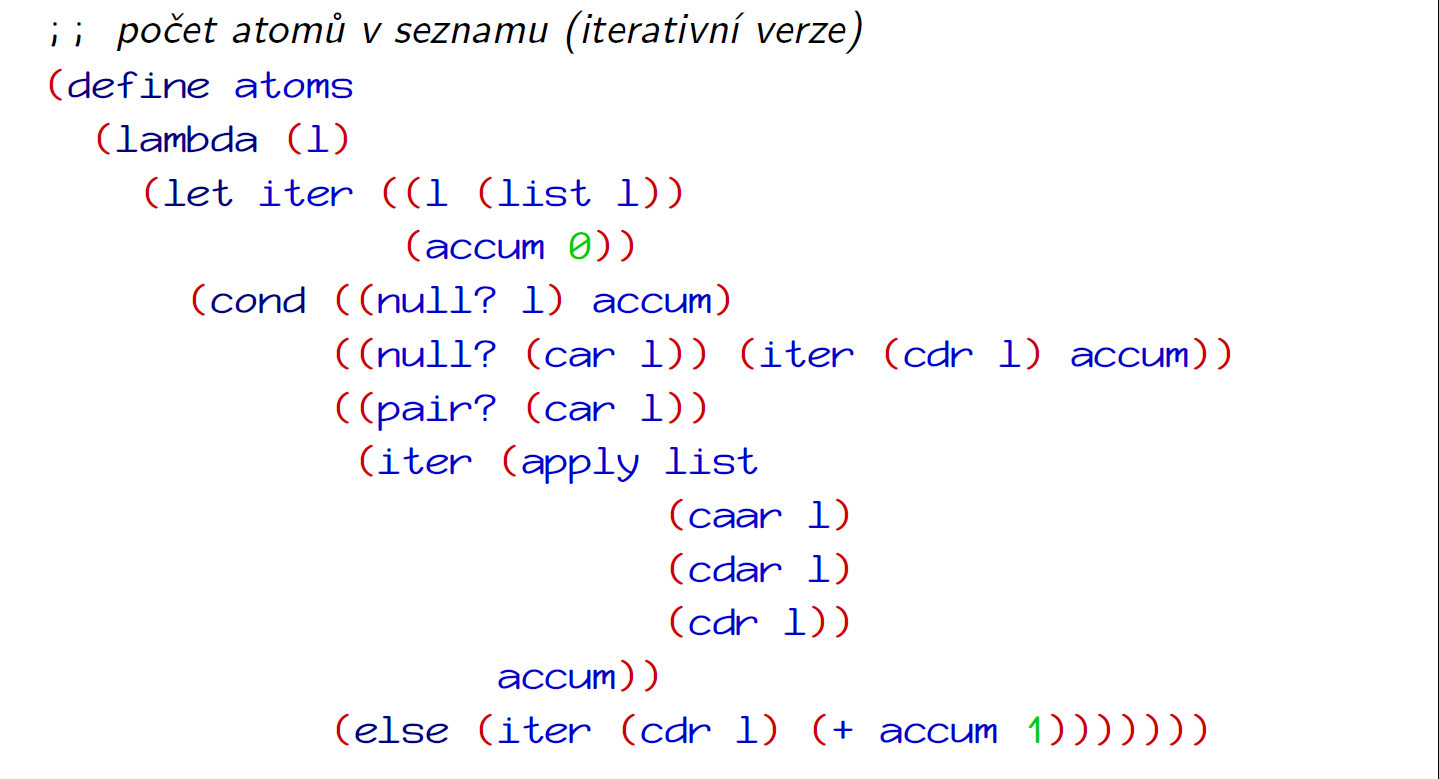
\includegraphics[scale=0.3]{img/zasobnikovy_model_3}
	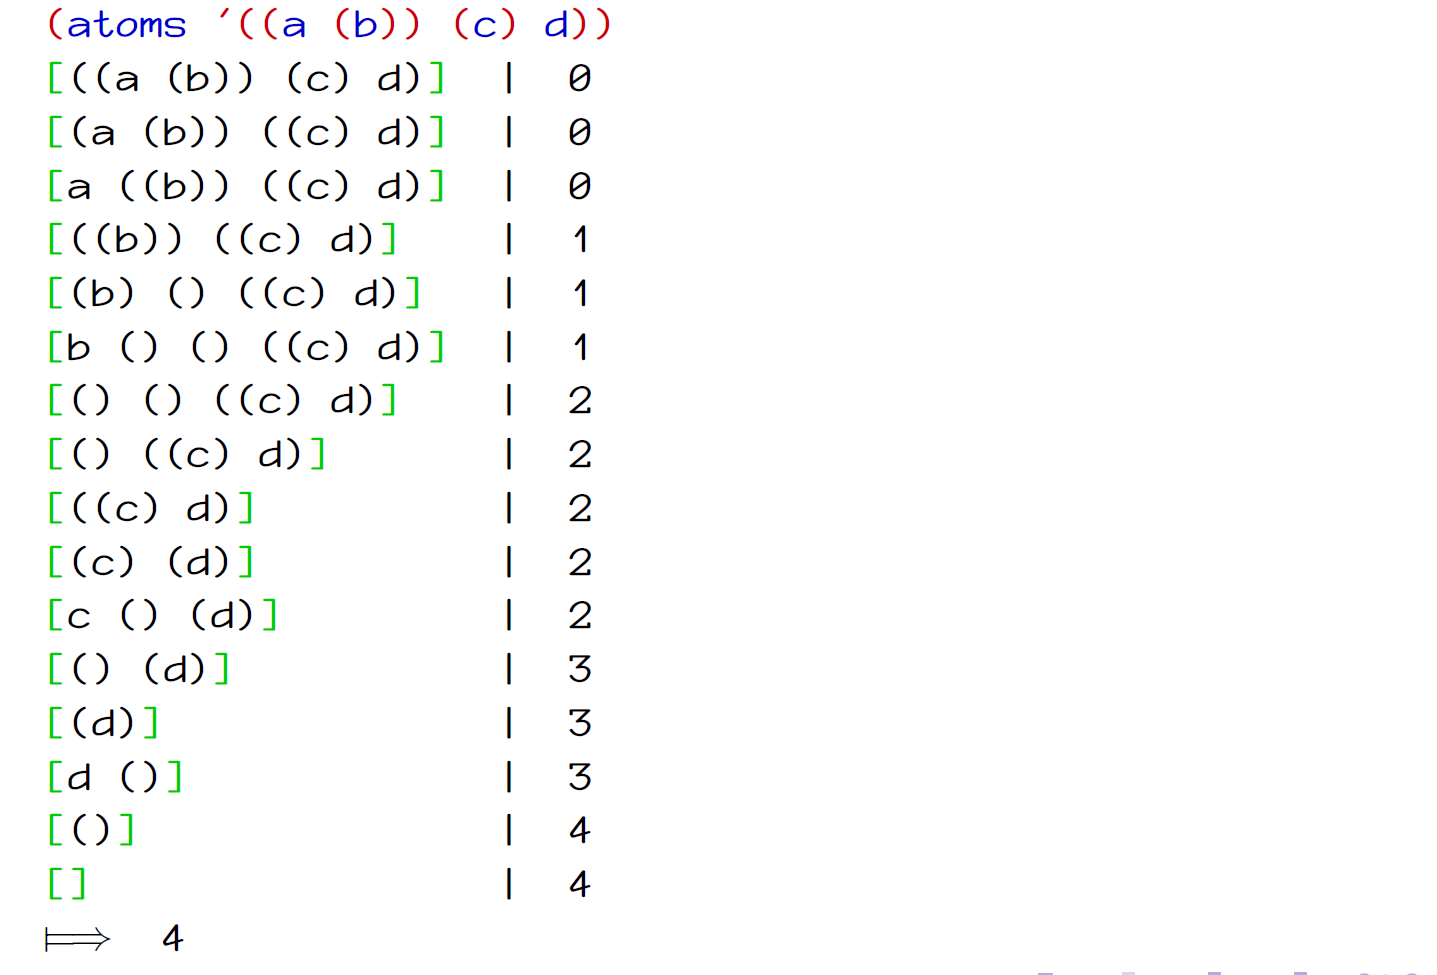
\includegraphics[scale=0.3]{img/zasobnikovy_model_4}
	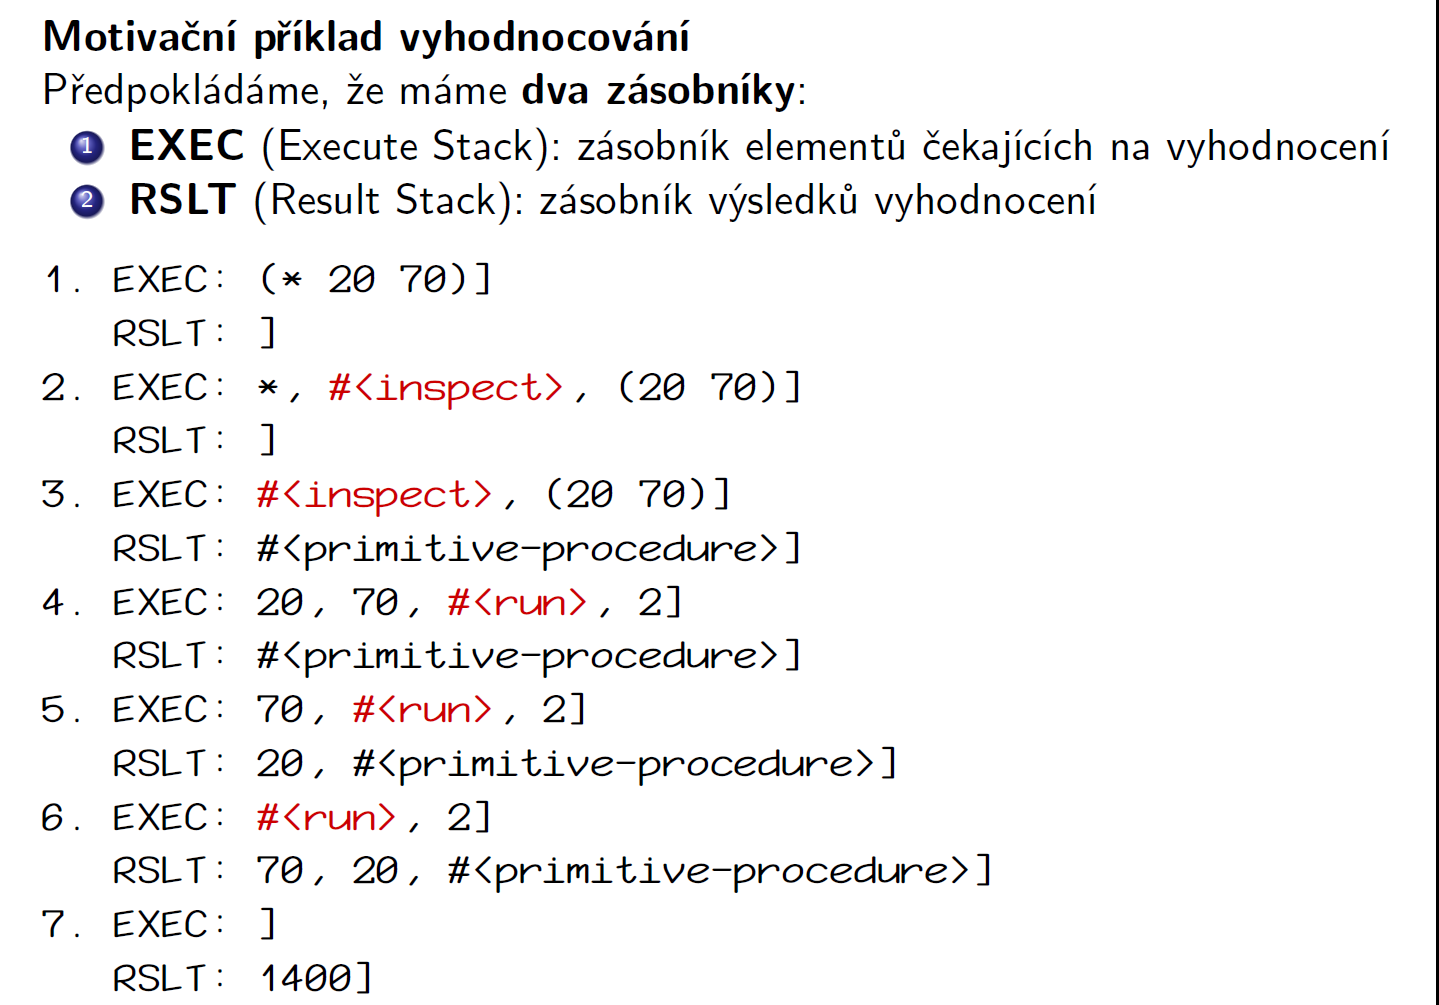
\includegraphics[scale=0.3]{img/zasobnikovy_model_5}
	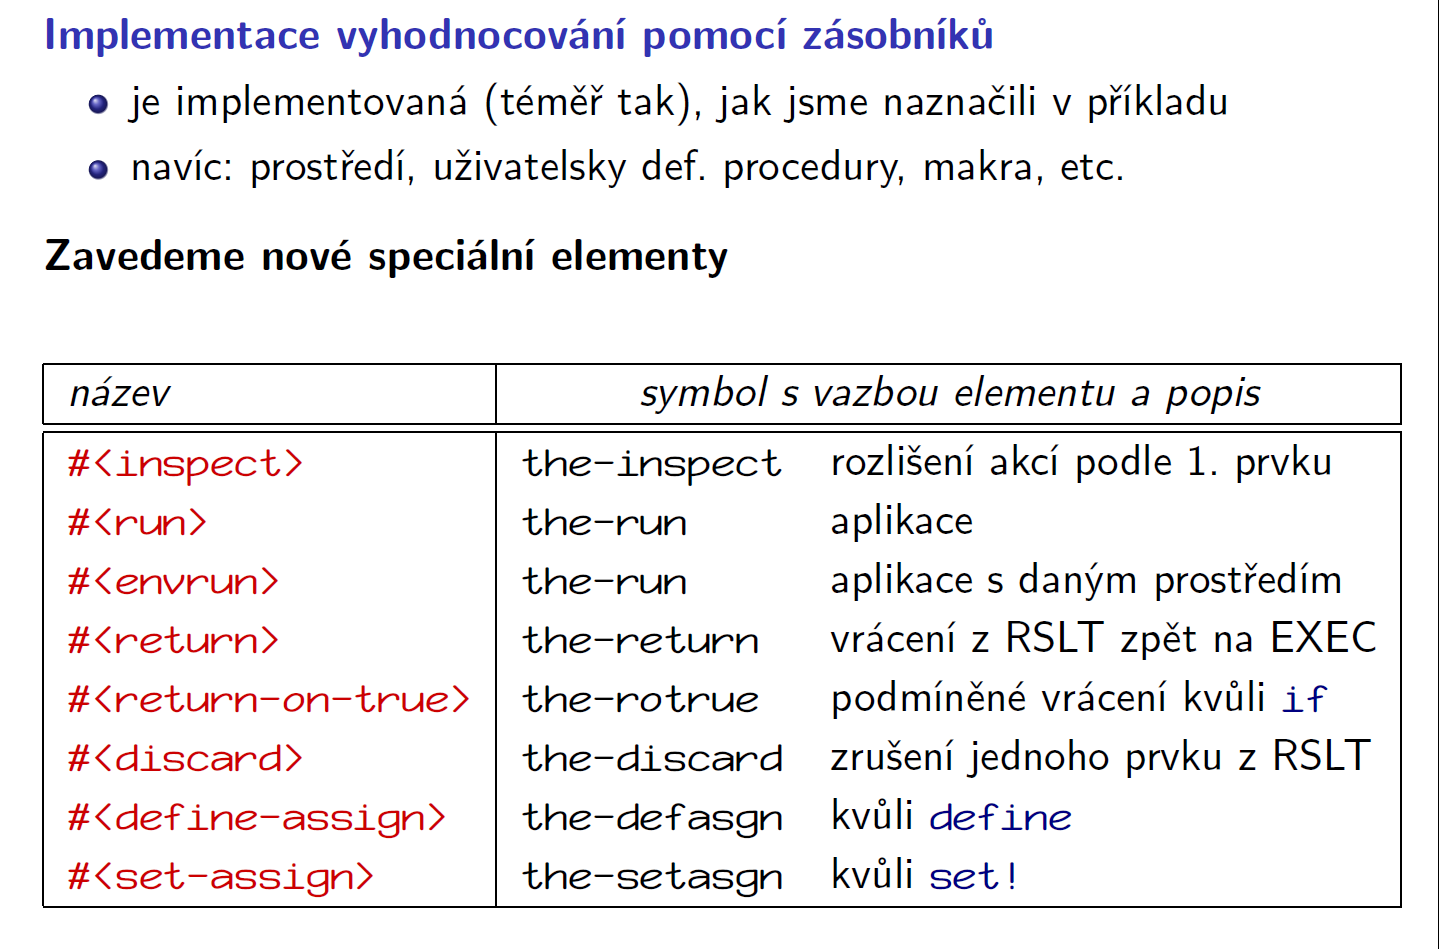
\includegraphics[scale=0.3]{img/zasobnikovy_model_6}
	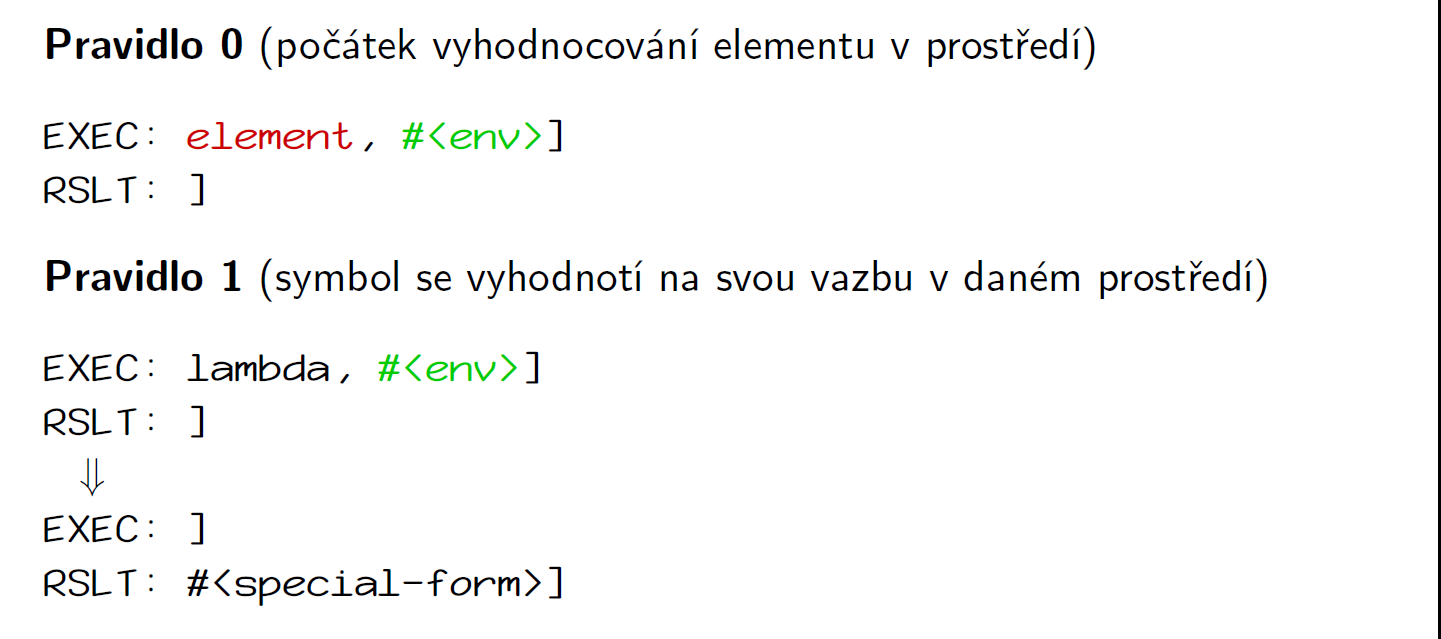
\includegraphics[scale=0.3]{img/zasobnikovy_model_7}
	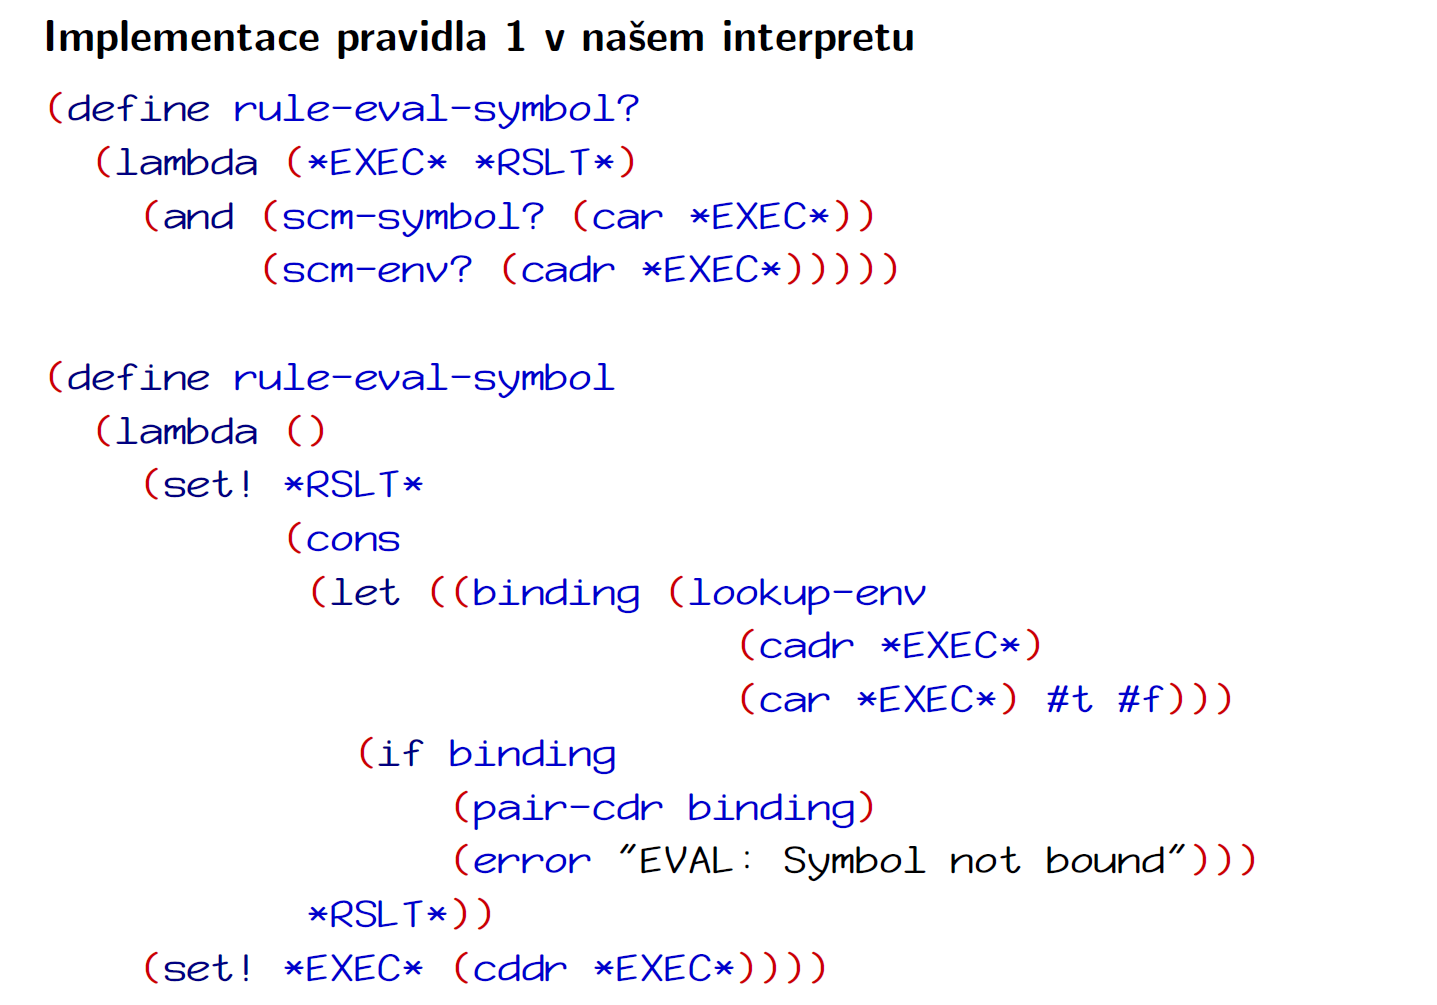
\includegraphics[scale=0.3]{img/zasobnikovy_model_8}
	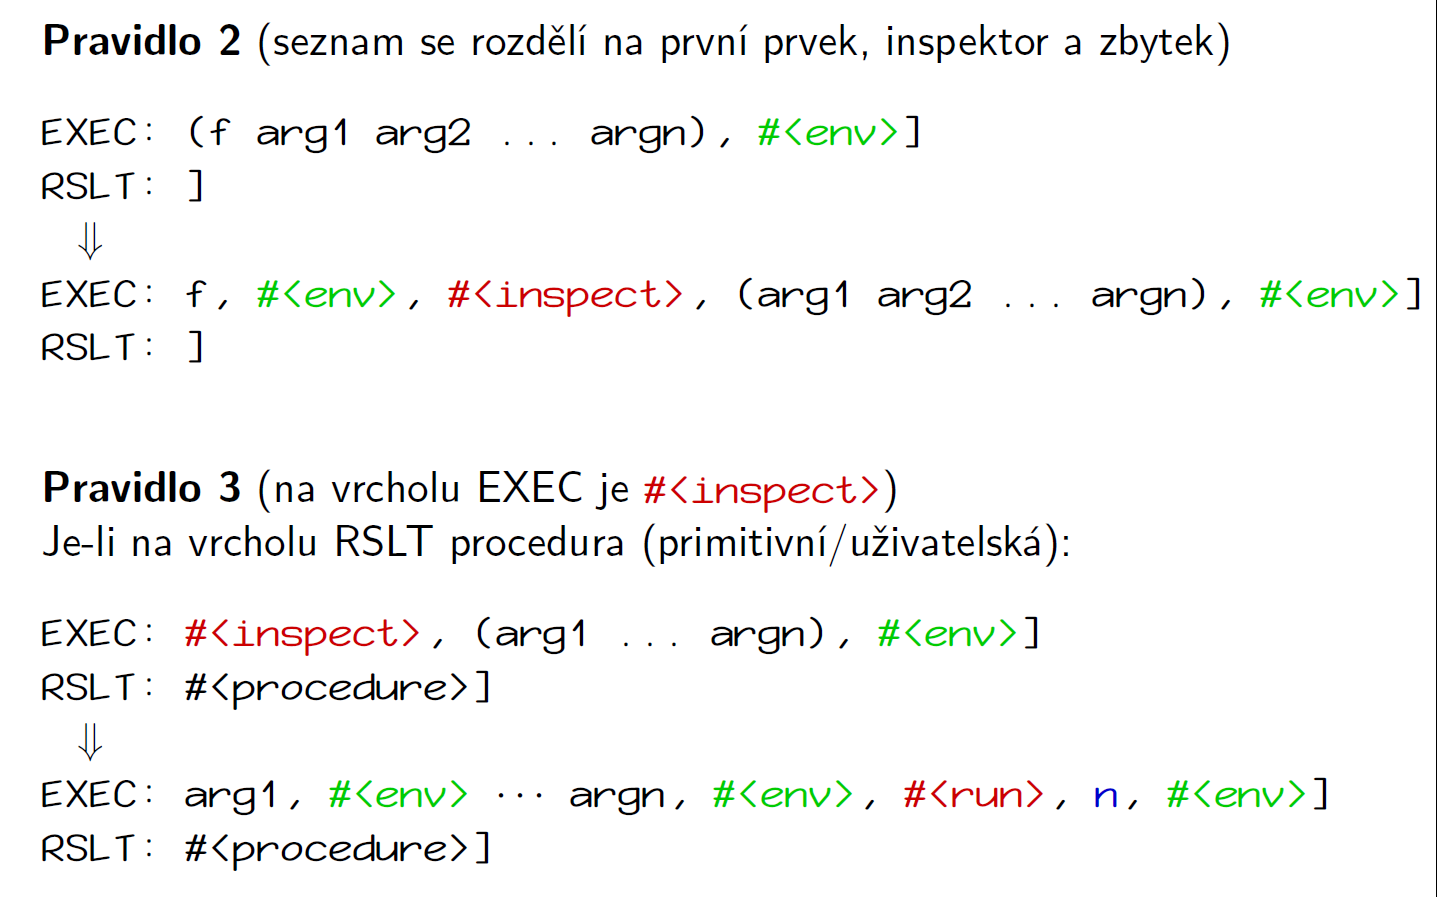
\includegraphics[scale=0.3]{img/zasobnikovy_model_9}
	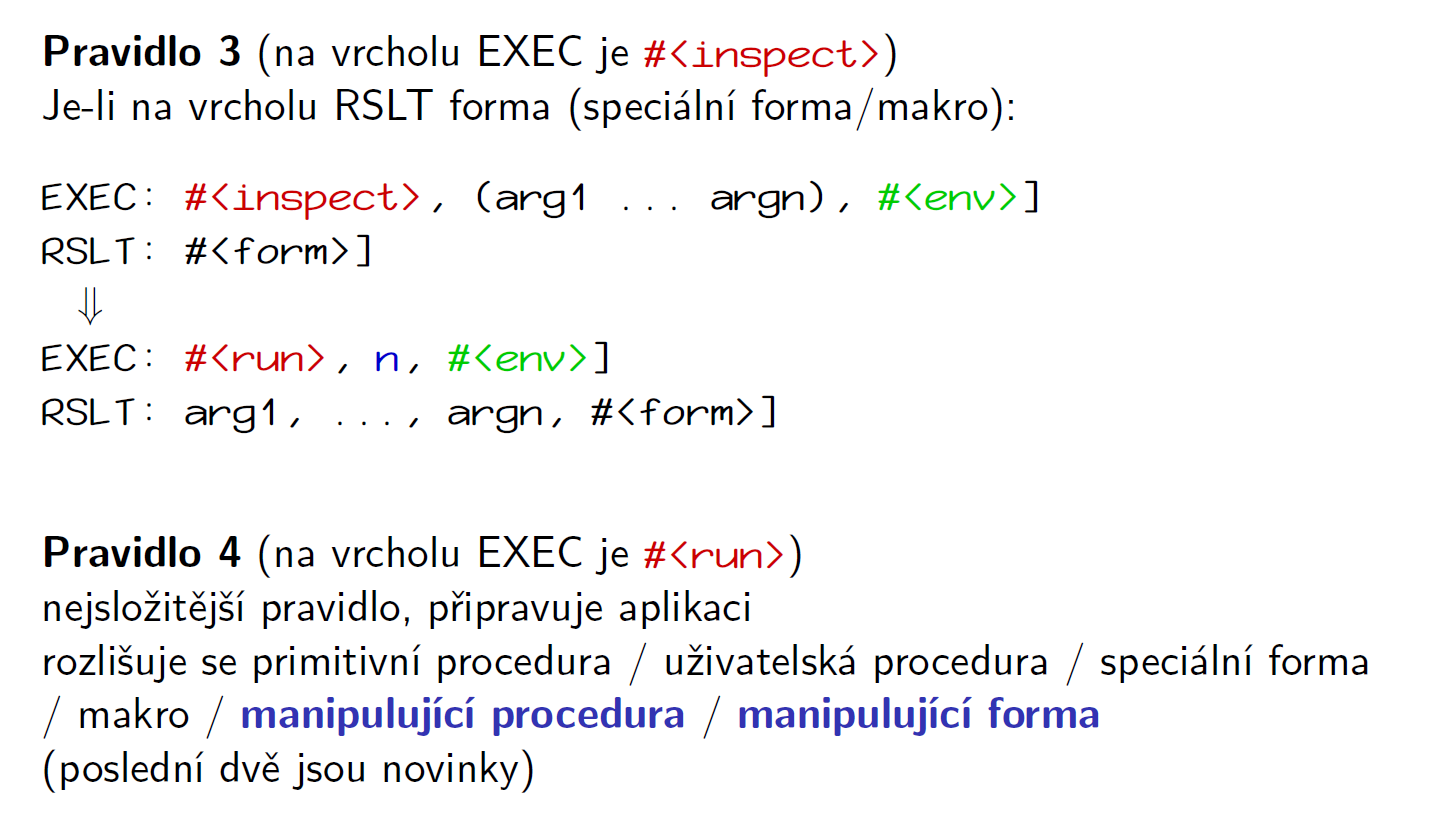
\includegraphics[scale=0.3]{img/zasobnikovy_model_10}
	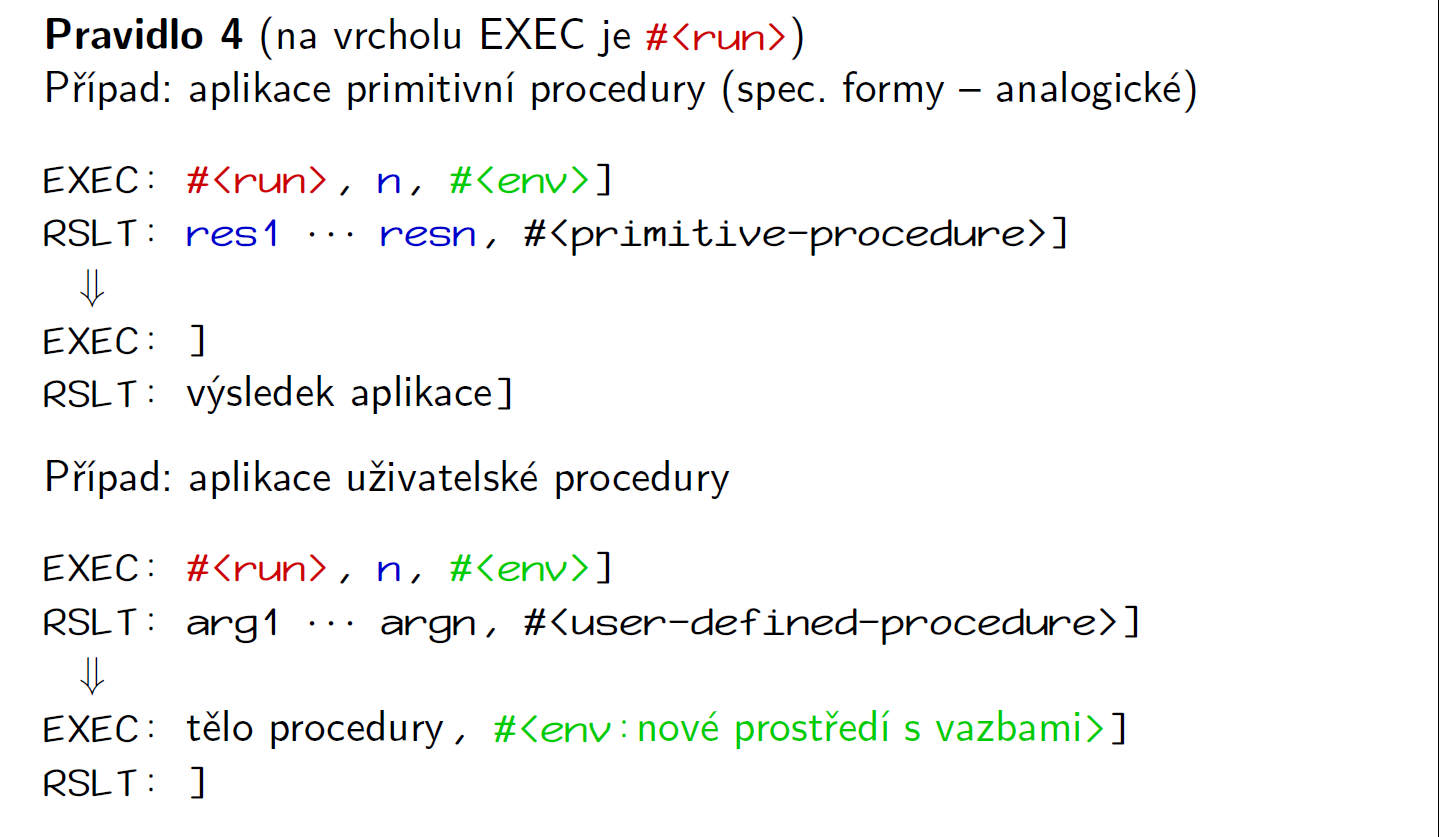
\includegraphics[scale=0.3]{img/zasobnikovy_model_11}
	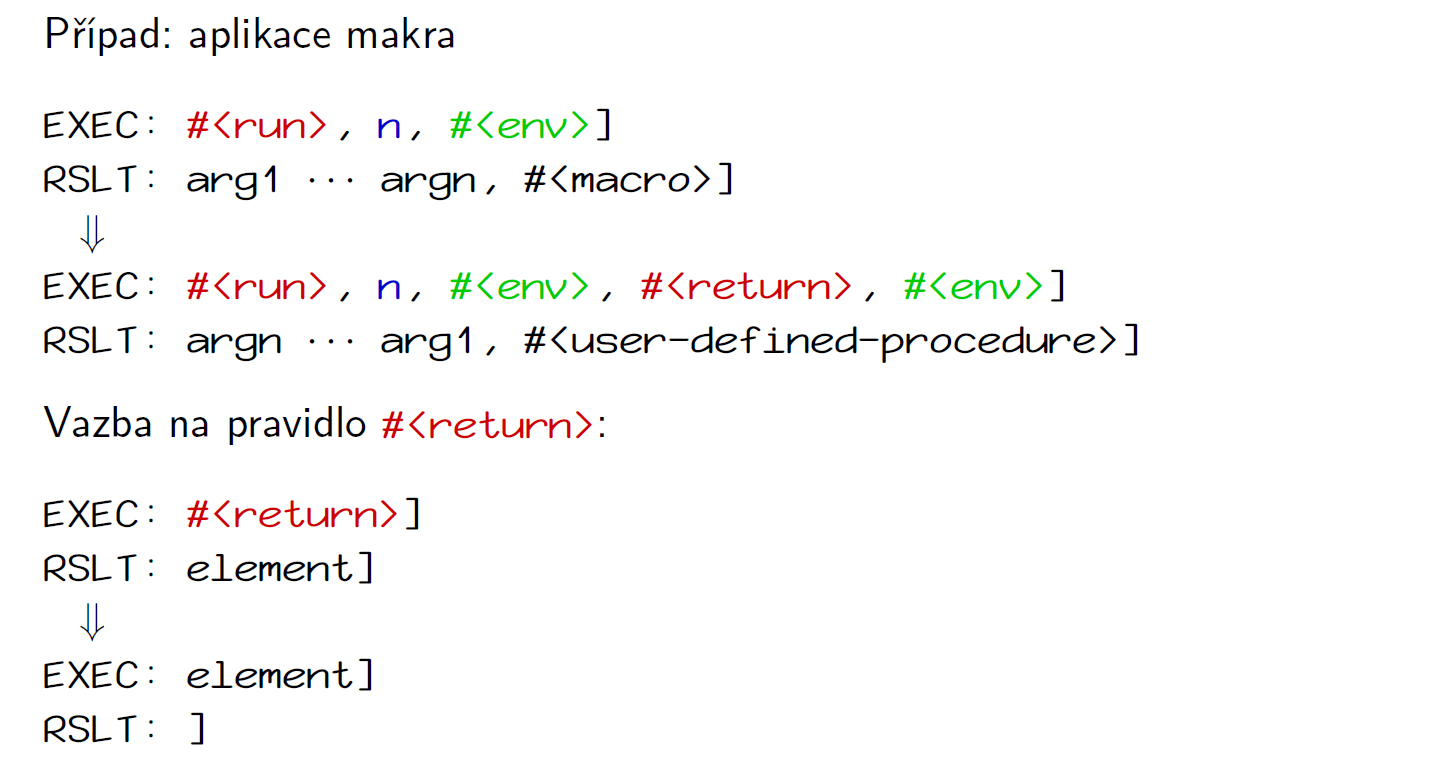
\includegraphics[scale=0.3]{img/zasobnikovy_model_12}
	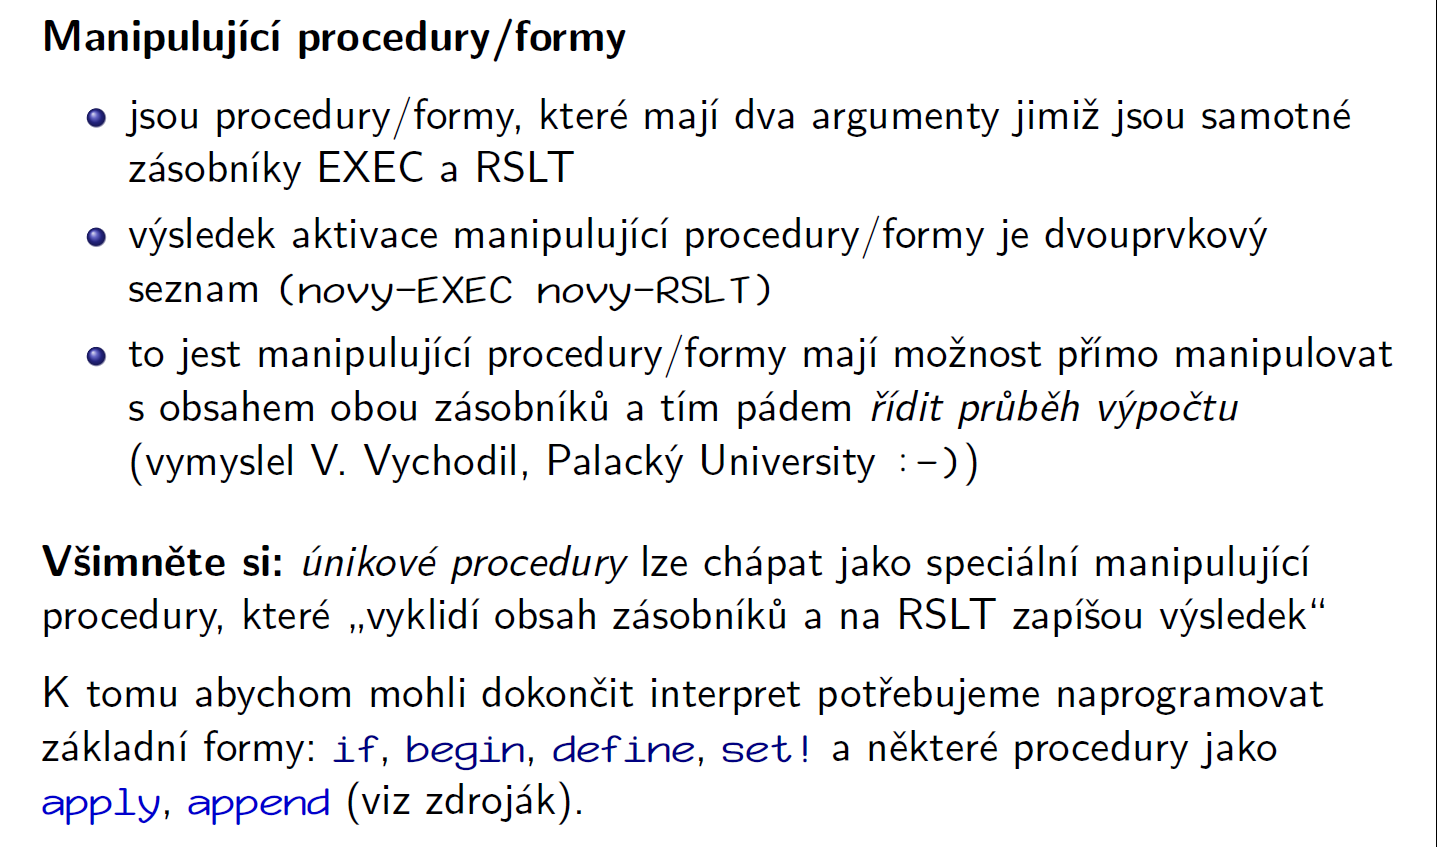
\includegraphics[scale=0.3]{img/zasobnikovy_model_13}
	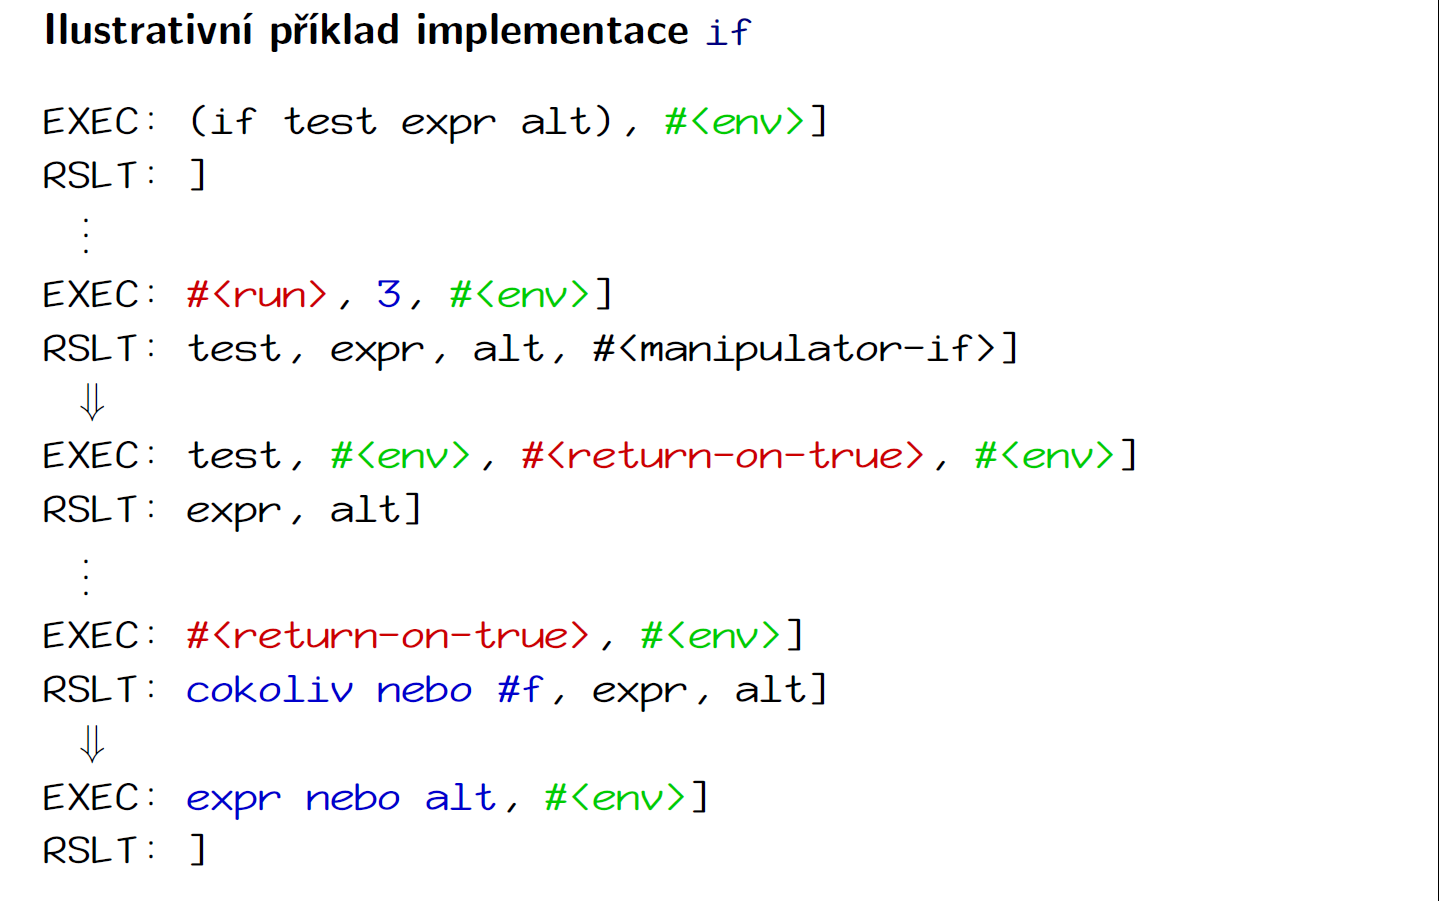
\includegraphics[scale=0.3]{img/zasobnikovy_model_14}
\end{center}









%---------------------------------------- Pátý odstavec---------------------------------------------------

\newpage
\section{Objektové programování}
	\paragraph{Objektové programování:} třídy a objekty, zprávy a metody. Zapouzdření, polymorfismus, dědičnost. Metody objektů, jejich typy, způsoby ochrany. Metody tříd, abstraktní třídy. Vícenásobná dědičnost, rozhraní. Příklady objektově orientovaných jazyků a jejich rysy.

	\subsection{Třídy a objekty, zprávy a metody}
		\subsubsection{Třída}
			Třída představuje předpis, na jehož základě budou vytvářeny objekty. Deklaruje atributy a definuje chování objektů dané třídy.

		\subsubsection{Objekt}
			Konkrétní instance dané třídy, nacházející se v daném stavu (nabývající konkrétní hodnoty) a poskytující rozhraní definované třídou.

		\subsubsection{Zprávy a metody}
			Zprávy a metody spolu úzce souvisejí. Metody vykonávají v rámci třídy (objektu) určitou funkcionalitu. Zprávy slouží pro komunikaci mezi objekty. V různých programovacích jazycích je tato funkcionalita implementována různě. Například v Javě se posílají zprávy voláním veřejných metod, C\# či Common Lisp využívají svůj systém posílání zpráv.


	\subsection{Zapouzdření, polymorfismus, dědičnost}
		\subsubsection{Zapouzdřední}
		Zapouzdření v objektech znamená, že k obsahu objektu se nedostane nikdo jiný, než sám vlastník. K okolí je objekt přístupný pouze pomocí definovaného rozhraní (metody daným způsobem zprostředkovávající, či modifikující, data objektu).

		\subsubsection{Dědičnost}
		Třídy jsou organizovány ve stromové hierarchii. Potomek třídy od svého rodičě přejímá (dědí) jeho metody a vlastnosti (public a protected). Zděděné metody lze překrýt vlastními implementacemi. Při tvorbě dědičnosti bychom se měli řídit pravidlem \textit{is-a}.

		\paragraph{is-a:} Mějme entity A, B. Třída reprezentující entitu B může dědit z třídy A pouze pokud je tvrzení \uv{B je A} pravdivé (i.e. \uv{Pes je Zvíře}).

		\paragraph{Vícenásobná dědičnost:} viz~\ref{vicenasobna-dedicnost} -- \nameref{vicenasobna-dedicnost}
		\\
		\\
		V některých programovaích jazycích může být třída prohlášena za neděditelnou pomocí klíčových slov \texttt{final} (Java), nebo \texttt{sealed} (C\#).

		\subsubsection{Polymorfismus}
		Situace, kdy několik objektů různých tříd poskytje stejné rozhraní a navenek se s nimi pracuje stejně, avšak jejich chování se liší dle implementace. Můžeme také hovořit o polymorfismu v souvislosti s dědičností -- jedná se o situaci, kdy je na nějakém místě očekáván objekt dané třídy, či libovolné třídy z ní odvozené. Rozhraní dané třídy je vždy podmnožinou rozhraní libovolné její potřídy.

	\subsection{Metody objektů, jejich typy, způsoby ochrany}
		\subsubsection{Metody}
			Metoda je ve třídě předepsaná pomocí:
			\begin{itemize}
				\item{Názvu metody}
				\item{Návratového typu -- u staticky typovaných jazyků}
				\item{Argumentů}
				\item{Modifikátoru přístupu -- \textbf{public} (lze volat odkudkoli), \textbf{protected} (lze volat pouze z metod stejné, či odvozené třídy), \textbf{private} (lze volat pouze z metod stejné třídy)}
				\item{Dodatečných atributů -- metody mohou být statické, abstraktní (virtuální), konečné (finální)}
			\end{itemize}

			\begin{note}
				Speciálním případem metod může být například konstruktor, destruktor, či gettery a settery.
			\end{note}

			Setkáváme se s pojmem \textbf{přetěžování metod}. Jedná se o situaci, kdy třída obsahuje více metod se stejným názvem. Takové metody se musí lišit počtem, nebo typem argumentů. Při volání metody je potom na základě argumentů zvolena požadovaná varianta.

		\subsubsection{Typy metod}
			Metody lze definovat jako:
				\begin{itemize}
					\item{statické -- kapitola~\ref{metody-trid}}
					\item{abstraktní (virtuální) -- kapitola~\ref{abstraktni-tridy}}
					\item{konečné (finální) -- Třída potomka je již nemůže předefinovat}
				\end{itemize}

		\subsubsection{Způsoby ochrany}
			Metody, stejně jako atributy objektu chráníme pomocí modifikátorů přístupu. Ty určují, odkud lze k metodám přistupovat.
			\begin{itemize}
				\item{\textbf{public} -- lze volat odkudkoli}
				\item{\textbf{protected} -- lze volat pouze z metod stejné, či odvozené třídy}
				\item{\textbf{private} -- lze volat pouze z metod stejné třídy}
			\end{itemize}

			\begin{note}
				Je-li metoda privátní, neznamená to, že ji může volat pouze objekt dané třídy pouze v rámci sebe samotného. Může tuto metodu volat i na jiném objektu stejné třídy.
			\end{note}

	\subsection{Metody tříd, abstraktní třídy}
		\subsubsection{Metody tříd}
			\label{metody-trid}
			Neplést s metodami objektů! Jedná se o metody k jejichž volání není potřeba vytvářet objekt dané třídy. Říkáme jim statické. Dle logiky věci nemohou tyto metody pracovat s daty konkrétního objektu. Nelze tedy přistupovat k hodnotám atributů, či volat ne-statické metody v rámci též třídy. Mohou však modifikovat proměnné třídy (neplést s vlastnostmi objektu), označované jako statické proměnné. Změna takovéto proměnné se projeví v rámci celého programu.
			\\
			\\
			Implementačně mohou být řešeny tak, že se při prvním volání metody dané třídy vytvoří speciální objekt této třídy, obsahující pouze statické metody a statické proměnné.

		\subsubsection{Abstraktní třídy}
			\label{abstraktni-tridy}
			Jedná se o třídy, z nichž nelze vytvořit objekt. Slouží ke generalizování vlastností a základního chování určité skupiny tříd (jejích potomků). Abstraktní třída může své metody libovolně buď implementovat, nebo označit za abstraktní. V tom případě pak ne-abstraktní potomek třídy musí dané metody implementovat.
			\\
			\\
			Hlavním rozdílem, mezi abstraktní třídou a rozhraním (\ref{rozhrani}) je to, že abstraktní třída může obsahovat implementace metod.

			\paragraph{Příklad:} Mějme dva typy databází – SQL databáze (Oracle, PostgreSQL, MySQL, atp.) a objektové databáze (např. MongoDB). Program chceme postavit tak, abychom mohli implementace (v tomto případě operací \texttt{select} a \texttt{insert}) jednoduše zaměňovat (pomocí polymorfismu).
			\\
			Z logiky věci vyplývá, že na vrcholu naší hierarchie bude rozhraní definující operace \texttt{select} a \texttt{insert}. Z něj pak budou dědit dvě větve tříd. První větev bude určena pro SQL databáze a jejím vrcholem bude abstraktní třída implementující metody \texttt{select} a \texttt{insert} obecným způsobem platným pro značnou část relačních databází. Z této třídu budou dědit jednotlivé implementace pro specifické databáze (a případně překryjí generické chování vlastní implementací).
			\\
			Druhou větví budou třídy určené pro jednotlivé objektové databáze. Ty bohužel žádnou abstraktní třídu mít nemohou, jelikož nemají žádný standardizovaný dotazovací jazyk.

	\subsection{Vícenásobná dědičnost, rozhraní}
		\subsubsection{Vícenásobná dědičnost}
			\label{vicenasobna-dedicnost}
			V některých programovacích jazycích může třída dědit z více rodičovských tříd současně. Jedná se například o C++, Common Lisp, Python,\dots Jazyky podporující pouze \uv{jednoduchou} dědičnost jsou například C\#, Java, nebo Ruby.
			\\
			\\
			Při použití vícenásobné dědičnosti narážíme zejména na problém zvaný \textit{The diamond problem}. Mějme třídy $A, B, C, D$, takové, že $B$ dědí $A$, $C$ dědí $A$ a $D$ dědí z obou $B$ i $C$. Nechť třídy $B$ a $C$ definují metodu $m$, zatímco $D$ ji nedefinuje. Zavoláme-li metodu $m$ na objektu třídy $D$, která její implementace bude zavolána? Různé jazyky tento problém řeší různě. Optimálním způsobem je využití C3 linearizačního algoritmu zvaného MRO (Method Resolution Order), který podle daných pravidel vytvoří lineárně uspořádaný graf a následně vybírá pouze dalšího následovníka v řadě.

		\subsubsection{Rozhraní}
			\label{rozhrani}
			Rozhraní je předpis tvořený seznamem metod splňujícím určitá kritéria.
			\begin{itemize}
				\item{Předepsané metody nemají implementaci (tělo), pouze hlavičku}
				\item{Předepsané metody nedefinují modifikátor přístupu. Metody musejí být následně implementovány jako veřejné}
			\end{itemize}
			Případně také může obsahovat konstanty.
			\\
			\\
			Pokud třída ve své definici říká, že implementuje dané rozhraní, pak to znamená, že implementuje \textbf{všechny} jeho metody. Jaké to má dopady na programování?
			\begin{itemize}
				\item{Můžeme se spolehnout, že objekty třídy implementující dané rozhraní, budou disponovat danou množinou metod}
				\item{Polymorfismus -- pokud máme objekty více tříd implementujících dané rozhraní, pak se budou metody vykonávající danou věc jmenovat stejně}
				\item{Návrhový vzor \textit{Program to an interface not an implementation} -- kód by neměl být závislý na konkrétní implementaci, ale měl by záviset na rozhraní. Potom by měl fungovat s libovolnou třídou implementující dané rozhraní}
			\end{itemize}

			\begin{note}
				Rozhraním nelze předepsat atributy objektu, pouze metody a konstanty.
			\end{note}

	\subsection{Příklady objektově orientovaných jazyků a jejich rysy}
		\subsubsection{Java}
			\begin{itemize}
				\item{Není čistě objektová -- obsahuje i primitivní datové typy}
				\item{Statické typování}
				\item{Pouze \uv{jednoduchá} dědičnost; Možnost implementovat více rozhraní}
				\item{Podporuje přetěžování metod}
				\item{Nepodporuje přetěžování operátorů}
				\item{Metody nejsou elementy prvního řádu; od Java 8 ale podporuje lambda výrazy}
			\end{itemize}

		\subsubsection{C\#}
			\begin{itemize}
				\item{Není čistě objektový -- obsahuje i primitivní datové typy}
				\item{Statické typování}
				\item{Podporuje přetěžování metod i operátorů}
				\item{Metody nejsou elementy prvního řádu, ale podporuje lambda výrazy}
			\end{itemize}

		\subsubsection{Smalltalk}
			\begin{itemize}
				\item{Čistě objektový}
				\item{Pouze \uv{jednoduchá} dědičnost}
				\item{Dynamické typování $\Rightarrow$ Nepodporuje přetěžování metod}
				\item{Řízení přístupu -- veřejné metody, soukromé data}
				\item{Všechny operace jsou řešeny zasíláním zpráv}
			\end{itemize}

		\subsubsection{Common Lisp}
			\begin{itemize}
				\item{Dynamický jazyk}
				\item{Objektový systém CLOS (Common Lisp Object System)}
				\item{Multiparadigmatický jazyk -- OOP je jedno z mnoha paradigmat, které lze kombinovat}
				\item{Dynamické typování $\Rightarrow$ Nepodporuje přetěžování metod}
				\item{Vícenásobná dědičnost}
				\item{Metody se definují mimo definici třídy}
			\end{itemize}

		\subsubsection{Python}
			\begin{itemize}
				\item{Multiparadigmatický}
				\item{Vícenásobná dědičnost -- linearizační algoritmus MRO}
				\item{Nepodporuje rozhraní}
				\item{Dynamické typování $\Rightarrow$ Nepodporuje přetěžování metod}
				\item{Nepodporuje řízení přístupu -- privátní vlastnosti a metody se označují pouze podtržítkem na začátku názvu}
				\item{Podporuje přetěžování operátorů}
				\item{Metody jsou elementy prvního řádu, podporuje lambda výrazy}
			\end{itemize}



%----------------------------------------treti odstavec---------------------------------------------------
\end{document}
